\documentclass[12pt]{book}
\usepackage{color}
\usepackage{fancyvrb}
\newcommand{\VerbBar}{|}
\newcommand{\VERB}{\Verb[commandchars=\\\{\}]}
\DefineVerbatimEnvironment{Highlighting}{Verbatim}{commandchars=\\\{\}}
% Add ',fontsize=\small' for more characters per line
\usepackage{framed}
\definecolor{shadecolor}{RGB}{248,248,248}
\newenvironment{Shaded}{\begin{snugshade}}{\end{snugshade}}
\newcommand{\AlertTok}[1]{\textcolor[rgb]{0.94,0.16,0.16}{#1}}
\newcommand{\AnnotationTok}[1]{\textcolor[rgb]{0.56,0.35,0.01}{\textbf{\textit{#1}}}}
\newcommand{\AttributeTok}[1]{\textcolor[rgb]{0.77,0.63,0.00}{#1}}
\newcommand{\BaseNTok}[1]{\textcolor[rgb]{0.00,0.00,0.81}{#1}}
\newcommand{\BuiltInTok}[1]{#1}
\newcommand{\CharTok}[1]{\textcolor[rgb]{0.31,0.60,0.02}{#1}}
\newcommand{\CommentTok}[1]{\textcolor[rgb]{0.56,0.35,0.01}{\textit{#1}}}
\newcommand{\CommentVarTok}[1]{\textcolor[rgb]{0.56,0.35,0.01}{\textbf{\textit{#1}}}}
\newcommand{\ConstantTok}[1]{\textcolor[rgb]{0.00,0.00,0.00}{#1}}
\newcommand{\ControlFlowTok}[1]{\textcolor[rgb]{0.13,0.29,0.53}{\textbf{#1}}}
\newcommand{\DataTypeTok}[1]{\textcolor[rgb]{0.13,0.29,0.53}{#1}}
\newcommand{\DecValTok}[1]{\textcolor[rgb]{0.00,0.00,0.81}{#1}}
\newcommand{\DocumentationTok}[1]{\textcolor[rgb]{0.56,0.35,0.01}{\textbf{\textit{#1}}}}
\newcommand{\ErrorTok}[1]{\textcolor[rgb]{0.64,0.00,0.00}{\textbf{#1}}}
\newcommand{\ExtensionTok}[1]{#1}
\newcommand{\FloatTok}[1]{\textcolor[rgb]{0.00,0.00,0.81}{#1}}
\newcommand{\FunctionTok}[1]{\textcolor[rgb]{0.00,0.00,0.00}{#1}}
\newcommand{\ImportTok}[1]{#1}
\newcommand{\InformationTok}[1]{\textcolor[rgb]{0.56,0.35,0.01}{\textbf{\textit{#1}}}}
\newcommand{\KeywordTok}[1]{\textcolor[rgb]{0.13,0.29,0.53}{\textbf{#1}}}
\newcommand{\NormalTok}[1]{#1}
\newcommand{\OperatorTok}[1]{\textcolor[rgb]{0.81,0.36,0.00}{\textbf{#1}}}
\newcommand{\OtherTok}[1]{\textcolor[rgb]{0.56,0.35,0.01}{#1}}
\newcommand{\PreprocessorTok}[1]{\textcolor[rgb]{0.56,0.35,0.01}{\textit{#1}}}
\newcommand{\RegionMarkerTok}[1]{#1}
\newcommand{\SpecialCharTok}[1]{\textcolor[rgb]{0.00,0.00,0.00}{#1}}
\newcommand{\SpecialStringTok}[1]{\textcolor[rgb]{0.31,0.60,0.02}{#1}}
\newcommand{\StringTok}[1]{\textcolor[rgb]{0.31,0.60,0.02}{#1}}
\newcommand{\VariableTok}[1]{\textcolor[rgb]{0.00,0.00,0.00}{#1}}
\newcommand{\VerbatimStringTok}[1]{\textcolor[rgb]{0.31,0.60,0.02}{#1}}
\newcommand{\WarningTok}[1]{\textcolor[rgb]{0.56,0.35,0.01}{\textbf{\textit{#1}}}}
\usepackage[nottoc]{tocbibind}
\usepackage{xspace}
%%%\usepackage[utf8]{inputenc}
\usepackage{titling}
\usepackage{sectsty}
\usepackage{indentfirst}
\usepackage[T1]{fontenc}
%\usepackage[ngerman]{babel}     %deutsche Silbentrennung
\usepackage[english]{babel}     %deutsche Silbentrennung
%\usepackage[automark]{scrpage2}
\usepackage{textcomp}
\usepackage{verbatim}
\PassOptionsToPackage{hyphens}{url}
\usepackage[colorlinks=true, linkcolor=blue, citecolor=red, urlcolor=blue]{hyperref}
\makeatletter
\g@addto@macro{\UrlBreaks}{\UrlOrds}
\makeatother
\usepackage{fancyhdr}
\usepackage[UTF8]{ctex}



\usepackage{soul}
\usepackage{makeidx}
\usepackage{emptypage}

% Chapter title style
\usepackage{titlesec}
\titleformat{\chapter}
   [display] %possible values are hang, leftmargin, drop, etc.
   {\Huge\bfseries} % format to be applied to the whole title
   {\MakeUppercase{\chaptertitlename} \thechapter} %label setting
   {0pt} %horizontal separation between label and title body
   {\MakeUppercase} %code preceding the title body
   [\vspace{1ex}\titlerule]

\usepackage{apacite}
\usepackage{amsmath}
\usepackage{amssymb}
%\usepackage{url}
%\usepackage{cite}
\usepackage[left=2.5cm, right=2.5cm, top=2.5cm, bottom=2.5cm]{geometry}
\geometry{headheight=27.2pt}
\usepackage{graphicx}
\usepackage{url}
\usepackage{float}
\usepackage{setspace}
\usepackage{subfigure}
\usepackage{titleref}
\usepackage{natbib}%[sort&compress]
%\usepackage[round,authoryear]{natbib}
\numberwithin{equation}{chapter}
\usepackage[bf]{caption}
\usepackage{multirow}
\usepackage{longtable}
\usepackage{booktabs} % 三线表
\usepackage[figuresright]{rotating}
\usepackage{multicol} %用于实现在同一页中实现不同的分栏
\usepackage{array} % 表格居中并且能够设置宽度
% 压缩pdf体积
%\pdfcompresslevel=9
%\pdfminorversion=5
%\pdfobjcompresslevel=3


\newcommand{\tabincell}[2]{\begin{tabular}{@{}#1@{}}#2\end{tabular}}
\renewcommand{\captionfont}{\small\slshape}
\renewcommand{\contentsname}{Contents}
\newenvironment{bottompar}{\par\vspace*{\fill}}{\clearpage}% move to the end of the page
%\renewcommand{\contentsname}{TABLE OF CONTENTS}
\addto\captionsenglish{% Replace "english" with the language you use
  \renewcommand{\contentsname}%
    {TABLE OF CONTENTS}%
}
\providecommand{\tightlist}{%
  \setlength{\itemsep}{0pt}\setlength{\parskip}{0pt}}


\renewcommand{\headrulewidth}{0pt}
\pagestyle{fancy}
%\setlength\bibindent{4em}

\begin{document}

%% -----------------------------------------------------------------------------
%% Title page
%% -----------------------------------------------------------------------------
\begin{titlepage}
\vspace{1cm}
\begin{center}
\linespread{2}\normalsize \bfseries \MakeUppercase{Modeling Truck Safety Critical Events: Efficient Bayesian Hierarchical Statistical and Reliability Models}
\end{center}

\vspace{7cm}

\begin{center}
{Miao Cai,  M.S.}\\
\vspace{0.3cm}
Draft on \today
\end{center}

\vspace{8cm}

\singlespacing
\begin{bottompar}
\begin{center}
Dissertation Presented to the Graduate Faculty of \\
Saint Louis University in Partial Fulfillment \\
of the Requirements for the Degree of\\
Public Health Studies, Ph.D.\\
\vspace{.5cm}
\the\year
\end{center}
\end{bottompar}

\linespread{2}
\end{titlepage}


%% -----------------------------------------------------------------------------
%% copy right page
%% -----------------------------------------------------------------------------
\cleardoublepage
\pagenumbering{roman}
\begin{bottompar}
\begin{center}
\textcopyright \xspace Copyright by\\
Miao Cai \\
ALL RIGHTS RESERVED\\
\vspace{.5cm}
\the\year
\end{center}
\end{bottompar}


\cleardoublepage
\topskip0pt
\vspace*{\fill}
\underline{COMMITTEE IN CHARGE OF CANDIDACY:}

\vspace{.3cm}
Professor Steven E. Rigdon, Ph.D.\\
{\setlength{\parindent}{20ex}  \indent \underline{Chairperson and Advisor}}

\vspace{.3cm}
Professor Hong Xian, Ph.D.

\vspace{.3cm}
Assistant Professor Fadel Megahed, Ph.D.
\vspace*{\fill}








\hypertarget{dedication}{%
\chapter*{Dedication}\label{dedication}}
\addcontentsline{toc}{chapter}{Dedication}

I dedicate this dissertation to my parents, Zhimin Cai (蔡致民) and Guizhen Xu (徐桂珍), who believe in the power of higher education, hard work, and always support me.

\hypertarget{acknowledgement}{%
\chapter*{Acknowledgement}\label{acknowledgement}}
\addcontentsline{toc}{chapter}{Acknowledgement}

I want to thank my PhD mentor and committee chair Dr.~Steven E. Rigdon, committee members Dr.~Hong Xian and Dr.~Fadel Megahed.

\linespread{1}
\cleardoublepage
\tableofcontents

\listoffigures
\listoftables

\mainmatter
\doublespacing

\hypertarget{introduction}{%
\chapter{INTRODUCTION}\label{introduction}}

\hypertarget{transportation-safety}{%
\section{Transportation safety}\label{transportation-safety}}

Traffic safety is a pressing public health issue that involves huge losses of lives and financial burden across the world.
As reported by the World Health Organization (WHO, \protect\hyperlink{ref-who2018}{2018}\protect\hyperlink{ref-who2018}{a}), road injury was the eighth cause of death globally in 2016, killing approximately 1.4 million people, which consisted of about 2.5\% of all deaths in the world.
If no sustained action is taken, road injuries are predicted to be the seventh leading cause of death across the world by 2030 (WHO, \protect\hyperlink{ref-who2018b}{2018}\protect\hyperlink{ref-who2018b}{b}).
Compared to the victims who were claimed lives by diseases, people killed in traffic are mostly early- or middle-aged, particularly those aged 4 to 44 years old (Evans, \protect\hyperlink{ref-evans2014traffic}{2014}; Litman, \protect\hyperlink{ref-litman2013transportation}{2013}).
Without traffic accidents, these victims could have much longer lives with normal quality of life

Apart from fatal deaths, road traffic injuries were also reported to be the cause of 50 million non-fatal life injuries and approximately 75.5 million disability-adjusted life years globally (Staton et al., \protect\hyperlink{ref-staton2016road}{2016}).
In high-income countries, the majority of non-death costs were attributable to non-fatal crashes, with 2\% of non-fatal events leading to over 40\% of life-time medical costs (Ameratunga et al., \protect\hyperlink{ref-ameratunga2006road}{2006}).
Besides non-fatal injuries, traffic safety is a major economic burden.
The global economic losses attributable to transportation safety were estimated to be 518 billion United States Dollars (USD), which accounted for 1\% the gross domestic product (GDP) in low-income countries, 1.5\% in middle-income countries, and 2\% in high-income countries (Dalal et al., \protect\hyperlink{ref-dalal2013economics}{2013}; Peden et al., \protect\hyperlink{ref-peden2004world}{2004}).

Specifically in the United States, transportation contributed to the highest number of fatal occupational injuries, leading to 2,077 deaths and accounting for over 40\% of all fatal occupational injuries in 2017 (The United States, Bureau of Labor Statistics, \protect\hyperlink{ref-bols}{2017}).
The National Safety Council reported that the number of deaths attributable to car crashes will be at least 40,000 in 2018, which is the third straight year that this number is over 40,000 (The National Safety Council, \protect\hyperlink{ref-nsc2018}{2018}).
Despite large amounts of investments in roads, improved vehicle protection and traffic policy implementation, and advanced emergency and trauma care, the reduction in traffic associated fatality rates is nominal (Litman, \protect\hyperlink{ref-litman2013transportation}{2013}).
If the change of traffic fatality rates in the US match those in other unremarkable countries, 20,000 traffic deaths could have been prevented each year (Evans, \protect\hyperlink{ref-evans2014traffic}{2014}).

The impact of road injuries is even more impactful in developing countries than in developed countries (Goonewardene et al., \protect\hyperlink{ref-goonewardene2010road}{2010}).
Although low- and middle-income countries own only 48\% of all the registered vehicles in the world, 90\% of road traffic fatalities and injuries were estimated to occur in these countries, which continue to be escalating due to rapid urbanization and motorization (Dalal et al., \protect\hyperlink{ref-dalal2013economics}{2013}; Staton et al., \protect\hyperlink{ref-staton2016road}{2016}).
Ten developing countries, including Brazil, Cambodia, China, Egypt, India, Kenya, Mexico, Russia, Turkey, and Vietnam, account for almost half of all the road traffic in the world (Hyder et al., \protect\hyperlink{ref-hyder2012addressing}{2012}).
For example, China has around 100,000 traffic-related fatalities each year (Zhang et al., \protect\hyperlink{ref-zhang2010road}{2010}), accounting for around 80\% of all accidental deaths, with 87\% of them caused by motor vehicles in 2015 (Jiang et al., \protect\hyperlink{ref-jiang2017transport}{2017}).
In comparison, 148,707 lives were claimed by road collisions in India in 2015, with the road fatality rate similar to the global average level of 17.4 deaths per 100,000 people (National Crime Records Bureau, Government of India, \protect\hyperlink{ref-india2015}{2015}).

\hypertarget{truck-safety}{%
\section{Truck safety}\label{truck-safety}}

In the US, the large commercial truck industry is the backbone of the economy. Approximately 70\% of freight is delivered via a truck at some point of their transportation, which account for 73.1\% of value and 71.3\% of volume of the domestic goods (Anderson et al., \protect\hyperlink{ref-anderson2017exploratory}{2017}; Olson et al., \protect\hyperlink{ref-olson2016weight}{2016}).
However, large trucks are associated with more catastrophic accidents among all vehicles, so they are the primary concern of traffic safety. In 2016, the Federal Motor Carrier Safety Administration (FMCSA) reported that 27\% fatal crashes in work zones involved large trucks (FMCSA, \protect\hyperlink{ref-fmcsareport2016}{2018}\protect\hyperlink{ref-fmcsareport2016}{a}). Among all 4,079 crashes involving large trucks or buses in 2016, 4,564 people (1.12 people per crash) were killed (FMCSA, \protect\hyperlink{ref-fmcsafacts2016}{2016}). Large truck crashes approximately claim 5,000 lives and cause 120,000 injuries each year, but only 15\% of these fatalities occur in the trucks, with a predominate 78\% occurred in the other vehicles (Neeley and Richardson Jr, \protect\hyperlink{ref-neeley2009effect}{2009}). Besides, the economic losses associated with large truck crashes are also higher than those with passenger vehicles, with an estimated average cost of 91,000 USD per crash (Zaloshnja et al., \protect\hyperlink{ref-zaloshnja2008unit}{2008}).

The high risk of large trucks is attributed to two aspects of reasons (Huang et al., \protect\hyperlink{ref-huang2013development}{2013}). First, large truck drivers generally need to drive alone for long routes, under on-time demands, and challenging weather and traffic conditions. Professional truck drivers usually need to work in shifts, and sometimes unavoidable late-night or early-morning shifts (Pylkkönen et al., \protect\hyperlink{ref-pylkkonen2015sleepiness}{2015}), which have been reported to be associated with sleep deprivation and disorders (Åkerstedt, \protect\hyperlink{ref-aakerstedt1988sleepiness}{1988}; Mitler et al., \protect\hyperlink{ref-mitler1997sleep}{1997}; Sallinen et al., \protect\hyperlink{ref-sallinen2005sleepiness}{2005}; Solomon et al., \protect\hyperlink{ref-solomon2004healthcare}{2004}). Besides, the long route, constant concentration, and overtime work, intertwine with sleep deprivation and disorder and induce the fatigue symptoms among truck drivers. It is estimated that fatigue among long distance truck drivers caused up to 31\% of single vehicle fatal truck crashes (Mitler et al., \protect\hyperlink{ref-mitler1997sleep}{1997}; National Transportation Safety Board, \protect\hyperlink{ref-ntsb1990}{1990}).

On the other hand, trucks have huge weights, large physical dimensions, and potentially carry hazardous cargoes. Although these huge-size trucks boost the transportation efficiency by increasing cargo capacity and reducing fuel costs per trip, they also raise public safety concerns (Lemp et al., \protect\hyperlink{ref-lemp2011analysis}{2011}). Large trucks can weight up to 80,000 pounds by federal law, which are twenty times as heavy as a normal-weight passenger vehicle (Department of Transportation, Utah, \protect\hyperlink{ref-utah2019}{2019}). If these trucks travel at the speed of 65 miles per hour on the highway, it will take them around 525 feet to stop, which is about two times the length of a football field (Department of Transportation, Utah, \protect\hyperlink{ref-utah2019}{2019}). The large physical size also creates large blind spots on both sides of the truck, which poses more threat on smaller-sized vehicles. When a crash occurs between a large truck and a smaller vehicle, the sheer size and weight of the truck result in the tragedy that the victims are from the smaller vehicle instead of from the trucks in around 80\% of the cases (Neeley and Richardson Jr, \protect\hyperlink{ref-neeley2009effect}{2009}). In even worse case, commercial trucks crashes can cause massive casualties and regional public health emergency when the carried hazardous materials are leaked (such as gasoline and sulfuric acid).

The importance of truck industry and the potential catastrophic consequences underscore the need to reduce crash risk and improve the safety of truck transportation.

\hypertarget{modern-truck-safety-studies}{%
\section{Modern truck safety studies}\label{modern-truck-safety-studies}}

To reduce the lives and economic losses associated with trucks, numerous studies attempted to accurately identify the risk factors for truck-related traffic crashes and make accurate prediction. However, there are several limitations of studies using crash data. First, traffic crashes are characterized by rare events (dozens to thousands of times fewer crashes than non-crashes) (Theofilatos et al., \protect\hyperlink{ref-theofilatos2018impact}{2018}, \protect\hyperlink{ref-theofilatos2016predicting}{2016}). To tackle this rare-event issue, the most common study design is a case-control study, which matches a crash with one to up to ten non-crashes, and then use statistical models such as logistic regressions to explain the causes or predict the crashes (Braver et al., \protect\hyperlink{ref-braver1997tractor}{1997}; Chen and Xie, \protect\hyperlink{ref-chen2014modeling}{2014}; Meuleners et al., \protect\hyperlink{ref-meuleners2015obstructive}{2015}; Née et al., \protect\hyperlink{ref-nee2019road}{2019}). Unfortunately, a case-control study is limited in estimating incidence rates or overall average treatment effect. It may be contentious in selecting the ratio of controls to cases and how to select these controls (Grimes and Schulz, \protect\hyperlink{ref-grimes2005compared}{2005}; Sedgwick, \protect\hyperlink{ref-sedgwick2014case}{2014}). Second, due to the retrospective nature of crash data, it is unrealistic to trace back to the real-time traffic, weather, and other environmental factors that were associated with the crashes. Most of crash data reported by police and associated drivers were subject to recall and misinformation bias (Girotto et al., \protect\hyperlink{ref-girotto2016professional}{2016}). Third, crashes are underreported, especially for those with no or minor injuries or economic losses (Ye and Lord, \protect\hyperlink{ref-ye2011investigation}{2011}). The National Highway Traffic Safety Adminitration estimated that 25\% of minor-injury crashes and 50\% of no-injury crashes were not reported, compared to nearly 100\% reporting rate for fatal crashes (Savolainen et al., \protect\hyperlink{ref-savolainen2011statistical}{2011}).

Past truck safety literature almost exclusively focused on crashes, while ignoring precursors to crashes. A precursor to crashes, also known as safety critical events (SCEs), adverse events, or near-miss crashes, is an emerging pattern or signature associated with an increasing chance of crashes (Janakiraman et al., \protect\hyperlink{ref-janakiraman2016discovery}{2016}; Saleh et al., \protect\hyperlink{ref-saleh2013accident}{2013}). Truck SCEs deserve more attention since they occur more frequently than crashes, potentially suggest fatigue and a lapse in performance, and can lead to catastrophic crashes (Dingus, Vicki L Neale, et al., \protect\hyperlink{ref-dingus2006development}{2006}).

\hypertarget{proposal}{%
\section{Proposal}\label{proposal}}

With the rapid development of modern technology, more real-time naturalistic driving and SCEs data have been collected by commercial truck companies (Janakiraman et al., \protect\hyperlink{ref-janakiraman2016discovery}{2016}). With advanced unobstrusive instrumentation, these data provide a unique opportunity to continuously study real-world driving performance and potential consequences (Dingus et al., \protect\hyperlink{ref-dingus2016driver}{2016}). Naturalistic driving data can be further used to examine the risk factors associated with truck crashes, by fusing high-resolution data on the risk factors, such as driver behavior, vehicle condition, traffic, weather, and road geometry (Guo, \protect\hyperlink{ref-guo2019statistical}{2019}).

This prospectus proposal focuses on Bayesian hierarchical statistical and reliability models based on a large truck naturalistic driving data. The three specific research aims are:

\begin{enumerate}
\def\labelenumi{\arabic{enumi})}
\tightlist
\item
  quantify the association between truck crashes and SCEs,
\item
  construct scalable Bayesian hierarchical statistical and reliability models for truck critical events,
\item
  innovate the non-homogeneous Poisson process (NHPP) with power law process (PLP) intensity function to account for short rests between different trips.
\end{enumerate}

I believe that this work will contribute to statistical theories in constructing scalable Markov chain Monte Carlo (MCMC) to perform Bayesian hierarchical statistical and reliability models. Realistically, these statistical models will provide insights into the relationship between crashes and SCEs, as well as SCEs and driver characteristics, traffic, weather, and other real-time driving environmental variables. These statistical models can be further used to provide data-driven evidence to optimize trucking routes, minimize unsafe driving behavior, and improve a safe driving environment.

\hypertarget{literature-review}{%
\chapter{LITERATURE REVIEW}\label{literature-review}}

\hypertarget{naturalistic-driving-studies-nds}{%
\section{Naturalistic Driving Studies (NDS)}\label{naturalistic-driving-studies-nds}}

Traditional truck crash prediction studies almost exclusively use data that ultimately trace back to post hoc vehicle inspection, interviews with survived drivers and witnesses, and police reports (Hickman et al., \protect\hyperlink{ref-hickman2018synthetic}{2018}; Stern et al., \protect\hyperlink{ref-stern2019data}{2019}). Despite these data can be in-depth and thorough, they have several inherent limitations. Firstly, truck crashes are extremely rare compared with non-crashes. According to the FMCSA (\protect\hyperlink{ref-fmcsareport2017}{2018}\protect\hyperlink{ref-fmcsareport2017}{b}), large truck and bus fatalities in 2017 were 0.156 per million travelled vehicle miles, which was a 6.8 percent increase from 2016. This rareness poses a challenge to infer unbiased estimates using traditional statistical models (Guo et al., \protect\hyperlink{ref-guo2010near}{2010}; Theofilatos et al., \protect\hyperlink{ref-theofilatos2018impact}{2018}). Secondly, truck crash data almost exclusively reply on post hoc police reports. Although these data are generally accurate and detailed, they are limited in determining the information of the driver in a meaningful time period leading up to the crash (Dingus et al., \protect\hyperlink{ref-dingus2011estimating}{2011}). Some of the critical factors, such as distraction, are not reported or cannot be determined due to a varitety of reasons (Dingus et al., \protect\hyperlink{ref-dingus2011estimating}{2011}), and these data were subject to recall bias even if they were reported. Thirdly, truck crashes are under-reported, particularly for no-injury and minor-injury crashes (Stern et al., \protect\hyperlink{ref-stern2019data}{2019}; Ye and Lord, \protect\hyperlink{ref-ye2011investigation}{2011}). It is estimated that 25\% of minor-injury and 50\% of non-injury crashes were not reported, while 100\% of fatal crashes were reported (Savolainen et al., \protect\hyperlink{ref-savolainen2011statistical}{2011}).

In light of these limitations, a growing number of naturalistic driving studies have been initiated worldwide to identify crash causation and improve traffic safety (Guo, \protect\hyperlink{ref-guo2019statistical}{2019}; Hickman et al., \protect\hyperlink{ref-hickman2018synthetic}{2018}; Klauer et al., \protect\hyperlink{ref-klauer2009comparing}{2009}).
NDS use unobstrusive devices, sensors, and cameras installed on vehicles to proactively collect frequent naturalistic driving behavior and and performance data under real-world driving conditions (Guo, \protect\hyperlink{ref-guo2019statistical}{2019}; Hickman et al., \protect\hyperlink{ref-hickman2018synthetic}{2018}). Compared with tradtional post-hoc crash data that are road segment-based, NDS collect driver-based data that are more useful in comparing the rate of SCEs under different circumstances. In addition, NDS data provide high-resolution driver behavior and performance data, which enable researcher to access data shortly prior to the occurance of crashes or SCE without information bias or selection bias (Guo et al., \protect\hyperlink{ref-guo2010near}{2010}). Third, collecting naturalistic data is considerably less costly and difficult per observation compared to tradtional crash data that involve human resource, interviews, and witnesses, so NDS generally collect a large amount of data, which creates both an opportunity and a challenge to researchers. Guo (\protect\hyperlink{ref-guo2019statistical}{2019}) provides an excellent review that compares empirical , naturalistic, and epidemiological data collection methods in traffic safety research.

The first large-scale NDS was the 100-Car Naturalistic Driving study conducted by the Virginia Tech Transportation Institute in the US (Dingus, Klauer, et al., \protect\hyperlink{ref-dingus2006100}{2006}; Neale et al., \protect\hyperlink{ref-neale2005overview}{2005}). Other well-known NDS projects include the second Strategic Highway Research Program (Ghasemzadeh and Ahmed, \protect\hyperlink{ref-ghasemzadeh2017probit}{2017}) and the UDRIVE NDS in Europe (Barnard et al., \protect\hyperlink{ref-barnard2016study}{2016}; Eenink et al., \protect\hyperlink{ref-eenink2014udrive}{2014}). There are also a few other NDS that target at specific populations, such as the 40-Teen NDS (Alden et al., \protect\hyperlink{ref-alden2016animal}{2016}), the Older Driver Fitness-to-Drive NDS (Guo et al., \protect\hyperlink{ref-guo2015older}{2015}), and the Commercial Truck Driver NDS (Sparrow et al., \protect\hyperlink{ref-sparrow2016naturalistic}{2016}).

\hypertarget{safety-critical-events-sces}{%
\section{Safety-Critical Events (SCEs)}\label{safety-critical-events-sces}}

Instead of collecting extremely rare vehicle crash data, NDS focus on safety-critical events (SCEs) and near-crash events, defined as events that used last-second successful evasive maneuver that avoided crashes (Dingus et al., \protect\hyperlink{ref-dingus2011estimating}{2011}). Although near-crashes or SCEs were not real crashes, a few studies suggested that they are highly correlated with crashes (Dingus et al., \protect\hyperlink{ref-dingus2011estimating}{2011}; Dingus, Klauer, et al., \protect\hyperlink{ref-dingus2006100}{2006}; Guo et al., \protect\hyperlink{ref-guo2010near}{2010}). The most commonly studied SCE is hard brakes (also knowns as hard-braking events or harsh braking), defined as a deceleration force higher than a pre-specified threshold, such as 0.3 g (Jansen and Simone Wesseling, \protect\hyperlink{ref-jansen2018harsh}{2018}; Mollicone et al., \protect\hyperlink{ref-mollicone2019predicting}{2019}).

A more formal definition of near-crash, or the more general accident precursor, in safety analysis and accident prevention field was proposed and analyzed in Saleh et al. (\protect\hyperlink{ref-saleh2013accident}{2013}). An accident precursor was defined as a chain of adverse events following an initial off-nominal event, which can result in an accident if compounded with additional adverse conditions (Saleh et al., \protect\hyperlink{ref-saleh2013accident}{2013}). A near-crash or near miss is a special case of accident precursor, with the feature of being close to a complete accident sequence. Accidence precursor has been widely studied in certain safety science in which the accidents are extremely rare, such as nuclear industry (Smith and Borgonovo, \protect\hyperlink{ref-smith2007decision}{2007}), chemistry (Phimister et al., \protect\hyperlink{ref-phimister2003near}{2003}), and aerospace industry (Kirwan et al., \protect\hyperlink{ref-kirwan2008human}{2008}).

The rationale for using near-crashes and SCEs as surrogates for crashes is Heinrich's Triangle. The Heinrich's Triangle assumes that less severe events are more frequent than severe events, and the frequency of severe events can diminish as that of less severe events decreases (Guo, \protect\hyperlink{ref-guo2019statistical}{2019}). The latter assumption can be quantitatively tested using crash and naturalistic driving data, but verifying the former assumption is challenging since the causal mechanism is complex and unknown (Guo et al., \protect\hyperlink{ref-guo2010near}{2010}). Applying SCEs in traffic safety studies to this Heinrich's Triangle can substantially increase the study sample size and may potentially enable the estimation of driving risk. However, a crucial question prior to the usage of SCEs in naturalistic studies is whether they are good surrogates of traffic crashes.

Guo et al. (\protect\hyperlink{ref-guo2010near}{2010}) proposed two critical principles for using near crashes as surrogates for crashes: 1) similar or the same causal mechanisms between crashes and surrogates, 2) a strong association between the frequency of surrogates and crashes. Based on the 100-car database, they investigated the two principles using a sequential factor analysis, a Poisson regression, and a sensitivity analysis. The study concluded that using near crashes as surrogates for crashes will lead to conservative risk estimates but significantly reduce the variance of estimation. They suggested that using near crashes as surrogates in small-scale studies will be informative for evaluating the risk of crashes.

\hypertarget{crashes-and-sces}{%
\section{Crashes and SCEs}\label{crashes-and-sces}}

The 100-Car NDS continuously followed 102 recruited drivers for 12 months, resulting in two million miles and over 40,000 hours of driving data. To maximize the number of SCEs, the research team intentionally chose more young drivers and high mileage drivers. Based on this data, Dingus, Klauer, et al. (\protect\hyperlink{ref-dingus2006100}{2006}) found that hard braking events were significantly associated with collisions and near-crashes. Since the number of near-crashes and incidents were significantly larger than crashes, they proposed to use near-crashes and incidents as surrogates of crashes.

Gordon et al. (\protect\hyperlink{ref-gordon2011analysis}{2011}) conducted a preliminary study to validate surrogates for road-departure crashes by spatially merging road geometry, average traffic, crashes, and naturalistic driving data. Bayesian seemingly unrelated Poisson models estimated with weighted least squares were used to examine if the same sets of predictor variables can have the same effects on crashes and surrogates respectively. The found that time to edge crossing and lane-departure warning were two useful surrogates for crashes on rural nonfreeway roads, while lane deviation was a poor surrogate for lane-departure crashes.

Simons-Morton et al. (\protect\hyperlink{ref-simons2012elevated}{2012}) examined whether elevated gravitational-force predicts crashes and near crashes among 42 newly licensed teenage drivers in Virginia. Using the Naturalistic Teenage Driving Study data that followed the recruited drivers for 18 months. A logistic regression estimated with generalized estimating equations to account for the within-subject correlation among different months. It was found that the rate of elevated gravitational-force events was positively associated with the rate of crashes and near-crashes (odds ratio = 1.07, 95\% confidence interval: 1.02, 1.12), with the area under curve (AUC) value of 0.76.

Wu and Jovanis (\protect\hyperlink{ref-wu2012crashes}{2012}) proposed a conceptual framework to estimate the crash-to-surrogate ratio \(\pi\) using the 100-Car study. The study found that the conditional probability of a crash was increased by 24 times with a lateral acceleration more than 0.7 g, but the probability was decreased by other factors such as the event occurring in daylight and dry pavement. A later study by Wu and Jovanis (\protect\hyperlink{ref-wu2013defining}{2013}) developed diagnostic procedures to screen crashes and near-misses under the NDS settings. The study applied their proposed framework to the 100-Car NDS and identified three conditions to define surrogate events: 1) maximum lateral acceleration difference of no smaller than 0.4 g, 2) non-intersection related, and 3) maximum lateral acceleration difference no smaller than 0.9 per event or between 0.8 and 0.9 g during night time.

Guo and Fang (\protect\hyperlink{ref-guo2013individual}{2013}) attempted to identify risk factors of driving at drivers level and predict high-risk drivers based on the 100-Car study. The study used a negative binomial regression to examine the potential four risk factors of crashes and near-crashes. Besides, they used a K-mean clustering to classify the drivers into high-, moderate-, and low-risk groups based on crash and near-crash rates, and applied two logistic regressions to predict high- or moderate-risk drivers. The results confirmed that critical-incident event rates were significantly associated with individual driving risk. The two logistic regressions achieved AUC values of 0.938 and 0.93. They also highlighted that it was a first-step study and more studies with larger and representative data were needed to confirm the association. A similar study by Wu et al. (\protect\hyperlink{ref-wu2014using}{2014}) also used the 100-Car study. This study used a Bayesian multivariate Poisson log-normal model to simultaneously account for crash frequency and severity. They also found a significant positive association between crashes, near crashes, and crash-relevant incidents.

Pande et al. (\protect\hyperlink{ref-pande2017preliminary}{2017}) used linear referencing to link Global Positioning System (GPS) data with roadway features on 39 segments of Highway 101 in California. A negative binomial model and a random-effects negative binomial model that account for segment-specific variance were used to investigate the relationship between historic crashes and hard braking. It was found that the freeway segments with high hard braking rates also had higher long-term crash rates, although the other three explanatory variables (average daily traffic, the presence of horizontal curvature, and auxiliary lanes) were not statistically significant.

Gitelman et al. (\protect\hyperlink{ref-gitelman2018exploring}{2018}) used in-vehicle data recorders (IVDR) data collected on 3,500 segments of inter-urban roads in Israel to examine the association between two types of safety-related events (braking and speed alert) and crashes on different road types. Negative binomial models were applied to account for the over-dispersion in the data, and they also included a number of road infrastructure characteristics as covariates. The number of braking events was found to be positively associated with injury crashes on single- and dual-carriageway roads while the association was not significant on freeways. However, they yield counterintuitive results that speed alert events (overspeed) were consistently and negatively associated with injury crashes on all road types. It was suggested that a speed alert event were not a good surrogate for crashes, possibly due to its rough definition.

Some researchers have been skeptical of NDS. Knipling (\protect\hyperlink{ref-knipling2015naturalistic}{2015}) challenged the validity of using naturalistic driving data and SCEs by stating that the purpose of traffic safety studies is to identify causes of crash harm, which is defined as property damage, injury, income lost, and all other consequences of different severities (Zaloshnja and Miller, \protect\hyperlink{ref-zaloshnja2007unit}{2007}). In contrast, NDS often use SCEs as surrogates of crashes, but very few or no crashes, let alone human harm. Therefore, Knipling (\protect\hyperlink{ref-knipling2015naturalistic}{2015}) argues that SCEs are not an appropriate part of the Heinrich's Triangle, so researchers generally cannot derive valid quantitative conclusions on causations of harm based on NDS datasets.

Another study by Knipling (\protect\hyperlink{ref-knipling2017threats}{2017}) specifically targeted Hour-of-Service rule research and relevant policy revisions among commercial truck drivers. He argued that HOS studies with a quasi-experiment design were subject to confounding variables, so these studies are limited in demonstrating a causal relationship between HOS and safety outcomes. The paper also argued that NDS lacked external validity since no large truck NDS had examined the causal link between crashed and SCEs. Lastly, the construct validity was doubted since the relationship between driver fatigue, HOS, and SCEs had not been validated.

\hypertarget{risk-factors-for-traffic-safety}{%
\section{Risk factors for traffic safety}\label{risk-factors-for-traffic-safety}}

\hypertarget{fatigue}{%
\subsection{Fatigue}\label{fatigue}}

Fatigue has been the most pressing risk factor for truck crashes and SCEs. It is estimated that approximately 32\% of drivers drive with fatigue over twice a month (National Sleep Foundation, \protect\hyperlink{ref-nsleepf}{2008}). The American Automobile Association Foundation for Traffic Safety claimed that 16.5\% of fatal traffic accidents and 12.5\% of injuries-related collisions were associated with driving with fatigue in 2010 (American Automobile Association Foundation for Traffic Safety, \protect\hyperlink{ref-aaafoundation}{2010}). The National Highway Traffic Safety Administration (NHTSA) estimated that 60\% of fatal truck crashes were attributable to the driver falling asleep while driving (Cavuoto and Megahed, \protect\hyperlink{ref-cavuoto2017understanding}{2017}; Craye et al., \protect\hyperlink{ref-craye2016multi}{2016}). The FMCSA estimated that the causal role of fatigue is around five times higher in fatal than in property damage truck crashes (Knipling, \protect\hyperlink{ref-knipling2017threats}{2017}).

Fatigue is often defined as a multidimensional process that leads to diminished worker performance, which may be a result of prolonged work, psychological, socioeconomic, and environment factors (Cavuoto and Megahed, \protect\hyperlink{ref-cavuoto2017understanding}{2017}; Yung, \protect\hyperlink{ref-yung2016fatigue}{2016}). However, this definition has low specificity since there are other factors associated with a decreased worker performance, such as cell phone use, which does not result in driver fatigue. There is no uniform and succint definition on fatigue since it involves interactions between biological, behavior, and psychological process. A comprehensive review on fatigue definition and measurement is provided by Yung (\protect\hyperlink{ref-yung2016fatigue}{2016}).

The mechanism of fatigue leading to SCEs is that the driver's capability to stay alert to ambient traffic and pedestrians will be largely impaired, and the driver's reaction time is subsequently prolonged in that situation (Zhang et al., \protect\hyperlink{ref-zhang2014study}{2014}). It is estimated that 17 hours of continuous working lead to a deterioration of driving performance equivalent to a blood alcohol level of 0.05\% (MacLean et al., \protect\hyperlink{ref-maclean2003hazards}{2003}). What makes the outcomes worse is that fatigue driving is more likely to happen on expressways and major highways where the speed limit is over 55 miles per hour (Knipling and Wang, \protect\hyperlink{ref-knipling1994crashes}{1994}). This is especially concerning because SCEs on these segments are more likely to result in serious injuries and fatalities, compared with non-fatigue driving safety critical events.

Although fatigue has been recognized as the primary reason for traffic safety, preventing drowsy driving has not been effective since there is no simple way to objectively measure fatigue driving (Dement, \protect\hyperlink{ref-dement1997perils}{1997}). In view of the difficulty of measuring fatigue, researchers attempted to use different proxies of fatigue associated with truck drivers, such as cumulative driving time, ocular and physiological metrics, sleep patterns, and night driving, but none of them has shown significant superiority.

Cumulative driving time has also been a measure of driver's fatigue level, especially among NDSs. For example, Nakayama (\protect\hyperlink{ref-nakayama2002trial}{2002}) found that there was a significant increase in the fatigue of drivers after 12 hours of continuous driving. Jovanis et al. (\protect\hyperlink{ref-jovanis2011hours}{2011}) used cumulative hours of driving, time of the day, driving patterns over multiple days, rests after driving, and the 34-hour recovery policy as measures of driver fatigue. They found that more driving time was associated with increased odds of crashes among 686 less-than-truck-load drivers, with the highest odds in the 11-th hour. From the fifth hour to the 11th hour, the odds of crashes were consistently increasing (Jovanis et al., \protect\hyperlink{ref-jovanis2012effects}{2012}). In contrast, Soccolich et al. (\protect\hyperlink{ref-soccolich2013analysis}{2013}) found no significant difference in safety outcomes between the 11-th driving hour and 8-, 9-, or 10-th driving hours using the Naturalistic Truck Driving Study data, but they suggested a working day that starts with several hours of non-driving work and then followed by 14 hours of driving was significantly associated with risk of SCEs. Another study by Mollicone et al. (\protect\hyperlink{ref-mollicone2019predicting}{2019}) used a Poisson regression to quantify the association between driver performance and predicted fatigue level based on natualistic driving data from 106 commercial truck drivers. The number of hard-braking events, defined as deceleration force greater than 0.3 g, were considered the outcome variable in that study. The fatigue level was predicted using a complex biomathematical model provided by McCauley et al. (\protect\hyperlink{ref-mccauley2013dynamic}{2013}). After accounting for time of the day, they reported a significant association between predicted fatigue and the rate of hard-braking events (relative risk 1.078, 95\% CI: 1.013-1.146).

Other studies used ocular metrics to detect driver's fatigue, such as eye closure and blinking patterns (Golias and Mishra, \protect\hyperlink{ref-golias2013evaluating}{2013}). For example, Jackson et al. (\protect\hyperlink{ref-jackson2016utility}{2016}) measured the eyelid closure of 22 healthy participants with 24 hours of sleep deprivation. They found a significant increase in proportions of time with closed eyeclids after the sleep deprivation, which were significantly associated with crashes, Psychomotor Vigilance Task lapses, and subjective sleepiness scores (95\% CI of Spearman's correlation coefficient was 0.46 to 0.69). Other studies used physiological measures, such as electroencephalogram (EEG) and heart rate, as indicators of fatigue (Golias and Mishra, \protect\hyperlink{ref-golias2013evaluating}{2013}). It has been demonstrated that awake but drowsy truck drivers during working have increased alpha and theta power densities in EEG (Cajochen et al., \protect\hyperlink{ref-cajochen1995power}{1995}; Kecklund and Åkerstedt, \protect\hyperlink{ref-kecklund1993sleepiness}{1993}; Mitler et al., \protect\hyperlink{ref-mitler1997sleep}{1997}). The variability of heart rates has been identified as a passive proxy of fatigue among drivers (Mulder, \protect\hyperlink{ref-mulder1992measurement}{1992}; Patel et al., \protect\hyperlink{ref-patel2011applying}{2011}).

Lack of sleep or specific sleep patterns have also been used as proxies of fatigue. For example, G. X. Chen et al. (\protect\hyperlink{ref-chen2016influence}{2016}) used negative binomial regression to identify the association between four sleep patterns and driving performance based on the Naturalistic Truck Driving Study data. They revealed that shorter sleep, early-stage sleep in a non-work period, and insufficient sleep between 1 am and 5 am were associated with increased safety-critical event rates. Sparrow et al. (\protect\hyperlink{ref-sparrow2016naturalistic}{2016}) reported that truck drivers with a retart break of only one nighttime period (defined as 1 am to 5 am) experienced more lapses of attention, elevated lane deviation at night, and higher sleepiness measured by subjective questionnaires. A naturalistic driving study by Wu et al. (\protect\hyperlink{ref-wu2014using}{2014}) found that more sleeping hours was found to be reducing near crashes.

A significant amount of research emphasizes the association between time of the day (such as night driving) and fatigue development (Cavuoto and Megahed, \protect\hyperlink{ref-cavuoto2017understanding}{2017}). Night drving is often accompanied by changes in shift scheduling, inadequate sleep, sleep apnea and disorder. For example, Pack et al. (\protect\hyperlink{ref-pack1995characteristics}{1995}) reported that the crashes caused by drivers falling asleep occurred primarily from mid-night to 7 am and from 2 pm to 4 pm. Mitler et al. (\protect\hyperlink{ref-mitler1997sleep}{1997}) monitored 80 truck drivers in North America using 24-hour electrophysiologic measures. They found that drivers had an average of 5.18 hours of sleep in bed and 4.78 hours of electrophysiologically validated sleep per day, which were significantly less than needed to stay alert on job. It was also suggested that late-night or early-morning work were detrimental to the drivers' sleep. Pahukula et al. (\protect\hyperlink{ref-pahukula2015time}{2015}) investigated the risk factors associated with crashes on Texas urban freeways between 2006 and 2010. They ran separate random-effects logistic regressions on five time periods: early morning (12 am to 4 am), morning (5 am to 9 am), mid-day (10 am to 3 pm), afternoon (4 pm to 8 pm), and evening (9 pm to 11 pm). The results suggested that different time periods contributed differently to the severity of injuries, which highlighted the importance of time of day.

\hypertarget{driver-characteristics}{%
\subsection{Driver characteristics}\label{driver-characteristics}}

Young and older drivers have been reported to have higher risk of crashes or SCEs. The reasons for young drivers having higher risk of driving are not fully explained, but could largely be attributed to inexperience and reckless driving. In contrast, older drivers may find it difficult to adjust for the sleep-wake cycle to keep pace with intense schedule required by their employer company, which may increase the likelihood to be sleepy or fatigued. Duke et al. (\protect\hyperlink{ref-duke2010age}{2010}) reviewed published literature on age-related safety issues among professional heavy vehicle drivers. The review suggested a U-shaped relationship: the chance of driving safety issues declines before 27 years old, plateau until the age of 63, and starts to grow up again after 63.

Young drivers are much better in the sense of physical health and resistance to fatigue compared with aged drivers. However, they are generally inexperience in driving compared with aged drivers. Clarke et al. (\protect\hyperlink{ref-clarke2006young}{2006}) suggested that young drivers (17--19 years old), especially males, have significantly more accidents than other drivers during the hours of darkness, on rural curves, and rear-end shunts compared to male drivers aged 20 -25 years. Campbell (\protect\hyperlink{ref-campbell1991fatal}{1991}) found that truck drivers under the age of 19 were over-involved in fatal accidents by a factor of 4, and those aged between 19 and 20 were over-involved by a factor of 6. Pack et al. (\protect\hyperlink{ref-pack1995characteristics}{1995}) revealed that the drivers under the age of 25 accounted for 55\% of the 4,333 crashes in which the drivers were judged to be asleep whiling driving. Otmani et al. (\protect\hyperlink{ref-otmani2005sleepiness}{2005}) tested the sleepiness of 36 profession drivers in simulated driving sessions using electroencephalogram, the Karolinska sleepiness scale, and visual analog scales. They found that young driver experienced a significant decrease in alertness and a strong tendency to sleep compared to middle-aged drivers. Based on the 100-Car Naturalistic Driving Study dataset, Wu et al. (\protect\hyperlink{ref-wu2014using}{2014}) found that drivers under the age of 25 were more likely to have crashes and SCEs.

To meet the huge demand services and supply chain management, it is common to extend retirement age or reemploy retired workers, especially in developing countries (Popkin et al., \protect\hyperlink{ref-popkin2008age}{2008}). Aged drivers have an increased chance of driving safety issues for three reasons: impaired eyesight, prolonged reaction time to exogenous stimuli, and vulnerability to fatigue (Di Milia et al., \protect\hyperlink{ref-di2011demographic}{2011}). Aged drivers often have eyesight diseases or functionality impairment, such as cataracts, narrowed peripheral vision and decreasing visual acuity (Di Milia et al., \protect\hyperlink{ref-di2011demographic}{2011}). In addition, working for truck companies often means irregular shifts and taking night schedules, which disrupt the circadian time-keeping systems, especially for aged workers (Moneta et al., \protect\hyperlink{ref-moneta1996time}{1996}). It is indicated that the ``critical age'' of shiftwork intolerance is about 45 to 50 years, at which sleep disorder, persisting fatigue and digestive problems become the most prominent (Di Milia et al., \protect\hyperlink{ref-di2011demographic}{2011}).

\hypertarget{traffic}{%
\subsection{Traffic}\label{traffic}}

Traffic characteristics are also viewed as an important risk factor for traffic safety issues. For the sake of availability and low cost, most prior studies used aggregated traffic data as proxies of traffic, such as Annual Average Daily Traffic (AADT). More recently, an increasing number of studies start to use real-time traffic data as a high-resolution proxy of traffic characteristics. Three published papers reviewed the impact of traffic variables on traffic safety issues (Roshandel et al., \protect\hyperlink{ref-roshandel2015impact}{2015}; Theofilatos and Yannis, \protect\hyperlink{ref-theofilatos2014review}{2014}; Wang et al., \protect\hyperlink{ref-wang2013effect}{2013}).

Traffic variables include flow (traffic volume), occupancy/density, and speed (Theofilatos and Yannis, \protect\hyperlink{ref-theofilatos2014review}{2014}; Wang et al., \protect\hyperlink{ref-wang2013effect}{2013}). Traffic flow is defined as the number of vehicles passing through a specific road segment in a given unit time. Traffic occupancy or density is defined as the number of vehicles in a unit area of road at a moment. Speed can be computed from the road perspective as the mean speed of vehicles passing that road segment (such as the AADT), or from the vehicle perspective as the speed of the vehicle (such as real-time speed). Compared to traffic flow and speed, traffic density is relatively less investigated due to a lack of relevant data.

For example, based on multinomial logit and negative binomial models, Dong et al. (\protect\hyperlink{ref-dong2017estimating}{2017}) used vehicle and driver characteristics, traffic, environment, and road geometry to predict the frequency and severity of large truck-involved crashes. They found that the percent of large trucks, AADT, driver condition, and weather characteristics were significantly associated with both crash frequency and severity. Theofilatos et al. (\protect\hyperlink{ref-theofilatos2018impact}{2018}) used hourly aggregated traffic variables, including flow, occupancy, mean time speed, and percentage of trucks to predict crash occurence with a bias-correction logistic regression. This study found that the main risk factor, average speed had a negative effect on crashes. Instead of studying risk factors of crashes, Kamla et al. (\protect\hyperlink{ref-kamla2019analysing}{2019}) examined the association between Hard Braking Incidents (HBIs) and geometric and traffic variables among large trucks at roundabouts. They found that HBIs were influenced by traffic and geometric variables in a similar fashion as crashes.

\hypertarget{weather}{%
\subsection{Weather}\label{weather}}

Weather variables, including precipitation, visibility, wind speed, and temperature, have have reported to have both direct and indirect effects on traffic safety events. Theofilatos and Yannis (\protect\hyperlink{ref-theofilatos2014review}{2014}) provides a review on weather characteristics and road safety.

Real-time extreme weather conditions such as heavy rain, fog, storm, and snow can either impair the driver's visual capability or reduce the safety of driving on the road (Al-Ghamdi, \protect\hyperlink{ref-al2007experimental}{2007}; Baker and Reynolds, \protect\hyperlink{ref-baker1992wind}{1992}; Chang and Chen, \protect\hyperlink{ref-chang2005data}{2005}). A positive linear relationship between precipitation and traffic accidents can be observed in both driver accidents and pedestrian accidents (Al-Ghamdi, \protect\hyperlink{ref-al2007experimental}{2007}; Graham and Glaister, \protect\hyperlink{ref-graham2003spatial}{2003}). Naik et al. (\protect\hyperlink{ref-naik2016weather}{2016}) used ordinal and multinomial regression models with random-effects to investigate crash severity under various weather conditions. They found that wind speed, rain, humidity, and temperature were associated with single-vehicle truck crashes. Abdel-Aty et al. (\protect\hyperlink{ref-abdel2012real}{2012}) used detector and sensor data to successfully predict more than 70\% of accidents with low visibility conditions.

In addition, the increase of ambient temperature places risks on occupational safety, and possibly leads to cognition loss, heat stroke, and impairment of wakefulness. Previous evidence showed that the risk of mistakes and SCEs are elevated in hot weather (Basagaña et al., \protect\hyperlink{ref-basagana2015high}{2015}; Kjellstrom et al., \protect\hyperlink{ref-kjellstrom2009direct}{2009}). Leard et al. (\protect\hyperlink{ref-leard2015weather}{2015}) found that for a day with temperature above 80 \(^{\circ}\)F, there is a 9.5\% increase in fatality rates compared with a day at 50-60 \(^{\circ}\)F. A review by Kampe et al. (\protect\hyperlink{ref-im2016impact}{2016}) found that 11 out of the 13 included studies indicated an increase in unintentional injuries associated with high temperatures. In constrast, when low temperature is present, truck drivers are likely to be faced with snowy or icy road conditions, as well as the presence of fog, which substantially increase the risk of driving (Lemp et al., \protect\hyperlink{ref-lemp2011analysis}{2011}). For example, Ahmed et al. (\protect\hyperlink{ref-ahmed2018effects}{2018}) reported that truck-involved crashes were 19\% more likely to occur than no truck-involved crashes when snow or strong wind were present.

\hypertarget{road-characteristics}{%
\subsection{Road characteristics}\label{road-characteristics}}

Based on engineering theory, road characteristics are potential risk factors of road safety (Wang et al., \protect\hyperlink{ref-wang2013effect}{2013}). Commonly used road characteristics in traffic safety studies include the number of lanes, lane with, speed limits, horizontal curves, road curvature, and lighting conditions.

The effect of the number of lanes and lane with on traffic safety is inconsistent in previous literature. Some studies suggest that the number of lanes is negatively associated with the risk of traffic accidents. For example, Zhu and Srinivasan (\protect\hyperlink{ref-zhu2011comprehensive}{2011}) found that crashes on roadways with more lanes tended to be less severe, which may result from the fact that more lanes give more space and separation between vehicles. They also reported that crashes in higher speed limit segments were more likely to be severe crashes. In contrast, several other studies suggested that an increase in the number of lanes and lane width were positively associated with traffic fatalities (Islam et al., \protect\hyperlink{ref-islam2014comprehensive}{2014}; Kononov et al., \protect\hyperlink{ref-kononov2008relationships}{2008}; Noland and Oh, \protect\hyperlink{ref-noland2004effect}{2004}; Zhu and Srinivasan, \protect\hyperlink{ref-zhu2011comprehensive}{2011}). This reversed relationship could possibly be explained by an increased chance of lane-change-related conflict opportunities (Wang et al., \protect\hyperlink{ref-wang2013effect}{2013}).

It is generally believed that lower speed limits can reduce the chances of traffic crashes, as well as the severity of crashes. For example, Neeley and Richardson Jr (\protect\hyperlink{ref-neeley2009effect}{2009}) used state-level data from 1991 to 2005 to examine the association between truck-specific restrictions and fatality rates. They found that higher speed limits were associated with increased fatality rates, although different speed limits across vehicle types had no significant effect. Another study by Davis et al. (\protect\hyperlink{ref-davis2015longitudinal}{2015}) also provided evidence that both overall and truck-involved fatalities were positively associated with maximum speed limits.

Road geometric design features, such as road curvature and terrain type, were also reported to be risk factor of traffic safety events. Dong et al. (\protect\hyperlink{ref-dong2015assessment}{2015}) used zero-inflated negative binomial models to examine the effects of road geometry features and crash frequency. Based on 1,787 truck-involved crashes from 1,310 highway segments in four years, they found that AADT, segment length, degree of horizontal curvature, terrain type, land use and width, median type, right side shoulder width, lighting condition, rutting depth, and posted speed limits were significantly associated with the likelihood of truck-involved crash frequency. Islam et al. (\protect\hyperlink{ref-islam2014comprehensive}{2014}) found that crashes on roadway curved were associated with higher likelihood of major and possible injuries in urban single-vehicle large truck at-fault accidents, but this association is not statistically significant in multi-vehicle accidents.

\hypertarget{predictive-models}{%
\section{Predictive models}\label{predictive-models}}

\hypertarget{overview}{%
\subsection{Overview}\label{overview}}

There are two cultures in current statistical or data science field: explanation and prediction (Breiman and others, \protect\hyperlink{ref-breiman2001statistical}{2001}; Shmueli and others, \protect\hyperlink{ref-shmueli2010explain}{2010}). The pro-explanation culture has long been adopted by most desciplines, such as epidemiology, economics, and psychology. In these desciplines, researchers commonly use generalized linear models, such as logistic regression and Poisson regression, to explain the association between the outcome and predictor variables. In contrast, the pro-prediction culture has recently been adopted in data science disciplines, in which they use blackbox algorithms such as random forests, decision trees, and neural networks to achieve similarly high prediction accuracy in training and testing sets. Pro-explanation models tend to excel at explaining the association between predictors and the outcome variable and being less likely to overfit the data. However, compared with machine learning and deep learning algorithms, pro-explanation models are less likely to capture potential interaction between predictor variables since they are driven by conceptual frameworks. Therefore, pro-explanation models generally have less prediction accuracy compared with black-box algorithms.

Traffic safety field has a pro-explanation culture, although it is shifting towards a pro-prediction by adopting cutting-edge machine learning and deep learning algorithms. The most commonly used statistical models in this field are logistic regression and Poisson regression. Logistic regression is commonly applied to predict crash likelihood (probability) using predictors such as driver features, weather, and traffic (Wang et al., \protect\hyperlink{ref-wang2017safety}{2017}). In contrast, Poisson regression is applied to predict the crash frequency (the number of crashes) within a time period using similarly aggregated traffic and weather characteristics. The following paragraphs will briefly introduce the two models and then compare the two cultures of predictive models in statistical and machine learning perspective.

The parameterization of a binary logistic regression is shown in Model \eqref{eq:logit}.
\begin{equation}
\begin{split}
Y_i & \sim \text{Bernoulli}(p_i) \\
\log(\frac{p_i}{1 - p_i}) & = \beta_0 + \beta_1x_1 + \beta_2x_2 + \cdots + \beta_kx_k
\label{eq:logit}
\end{split}
\end{equation}
Where \(Y_i\) is a binary variable that indicates whether an event occurred or not for the \(i\)-th observation. \(p_i\) is the mean parameter of a Bernoulli distribution, which is constrained on \([0, 1]\). The logit transformation of \(p_i\) then has the range from \(-\infty\) to \(+\infty\), which equals a linear combination of the predictors \(x_1, x_2, \cdots, x_k\) and associated parameters \(\beta_0, \beta_1, \cdots, \beta_k\).

The most commonly used outcomes for binary logistic regressions are injury versus non-injury crashes or fatal versus non-fatal crashes (Savolainen et al., \protect\hyperlink{ref-savolainen2011statistical}{2011}). For example, Cong Chen et al. (\protect\hyperlink{ref-chen2016driver}{2016}) used a two-level hierarchical Bayesian logistic model to predict the likelihood of high-severity crashes compared to low-severity crashes in New Mexico, accounting for both crash- and driver-level effects. They found that road curve, functional and disabled vehicle damage, single-vehicle crashes, female, older drivers, drug or alcohol involvement were associated with increased odds of severe crashes. Theofilatos et al. (\protect\hyperlink{ref-theofilatos2016predicting}{2016}) used logistic regression with rare events bias correction and Firth method to study significant risk factors for crashes in Greece. They found a negative association between crash likelihood and speed in crash locations. The proportion of trucks on the road was included in their model but not found to be significant. Other traffic safety studies using logistic regressions include but were not limit to Moudon et al. (\protect\hyperlink{ref-moudon2011risk}{2011}), Meuleners et al. (\protect\hyperlink{ref-meuleners2017determinants}{2017}), Ahmed et al. (\protect\hyperlink{ref-ahmed2018effects}{2018}). There are two excellent systematic reviews on traffic crash likelihood predictions by Roshandel et al. (\protect\hyperlink{ref-roshandel2015impact}{2015}) and Xu et al. (\protect\hyperlink{ref-xu2015calibration}{2015}).

Other variants of binary logistic regression are binary probit models (Lee and Abdel-Aty, \protect\hyperlink{ref-lee2008presence}{2008}; Yu and Abdel-Aty, \protect\hyperlink{ref-yu2014using}{2014}), ordered logistic or probit models (Xie et al., \protect\hyperlink{ref-xie2009crash}{2009}; Zhu and Srinivasan, \protect\hyperlink{ref-zhu2011comprehensive}{2011}), multinomial logit models (Ye and Lord, \protect\hyperlink{ref-ye2011investigation}{2011}). There are only minor difference between a probit model and a logistic model. A logistic model uses the inverse logit of the linear predictors to calculate the probability of an event, as shown in Equation \eqref{eq:inverselogit}; a probit model uses the cumulative normal density function of the linear predictors to calculate the probability, as shown in Equation \eqref{eq:probit}. The error function \(\text{erf}(x)\) is an integral without an analytical solution: \(\text{erf}(x) = \frac{2}{\pi}\int_0^xe^{-t^2}dt\).
\begin{equation}
p = \text{logit}^{-1}(\mathbf{X}^\prime\beta) = \frac{\exp (\mathbf{X}^\prime\beta)}{1 + \exp (\mathbf{X}^\prime\beta)}
\label{eq:inverselogit}
\end{equation}
\begin{equation}
p = \Phi(\mathbf{X}^\prime\beta) = \frac{1}{2}\Big[1+\text{erf}(\frac{\mathbf{X}^\prime\beta}{\sqrt 2})\Big]
\label{eq:probit}
\end{equation}
Ordered logistic or probit regressions aim to model an ordered multi-category outcome variable. The most common case is study the severity of crashes, such as no-injury crashes, minor-injury crashes, and fatal-injury crashes (Zhu and Srinivasan, \protect\hyperlink{ref-zhu2011comprehensive}{2011}). These ordered models account for the ranked nature of different severity levels but make the proportional odds assumption (Rifaat et al., \protect\hyperlink{ref-rifaat2012severity}{2012}). When the proportional odds assumption is violated, researchers often switch to multinomial logit or probit models, in which the outcome variable is deemed as nominal.

When researchers have crash data that are aggregated over a long time period such as one year, it often makes sense to study the number of crashes instead of whether a crash occurred or not since they are often more than one crash. The most commonly used statistical model is therefore Poisson model, as it well handles count data that are right-skewed, long tailed, and only have non-negative integer values. The parameterization of a Poisson regression is shown in model\eqref{eq:poisson}.
\begin{equation}
\begin{split}
Y_i^\star & \sim \text{Poisson}(\mu_i) \\
\log\mu_i & = \beta_0 + \beta_1x_1 + \beta_2x_2 + \cdots + \beta_kx_k,
\label{eq:poisson}
\end{split}
\end{equation}
where \(Y_i^\star\) is the number of events for the \(i\)-th observation, which must be a non-negative integer. \(\mu_i\) is both the mean and the variance parameter of the Poisson distribution, and it must be a non-negative numeric value. The logarithm of \(\mu_i\) transforms \(\mu_i\) into the range of \((-\infty, +\infty)\), which equals a linear combination of the predictors \(x_1, x_2, \cdots, x_k\) and associated parameters \(\beta_0, \beta_1, \cdots, \beta_k\). Note that the mean parameter equals the variance parameter in a Poisson distribution, which is often violated in real-life data. When the variance of the data is greater than expected, it is called overdispersion. Otherwise, it is called underdispersion. Overdispersion is much more common than underdispersion in practice.

Here are some applications of Poisson regression in traffic safety research. Cantor et al. (\protect\hyperlink{ref-cantor2010driver}{2010}) used Poisson regressions to explore the association between the rate of crashes driver-level characteristics among 560,695 commercial truck drivers in the United States. They found that past safety performance, out-of-service rate, body mass index (BMI), age, and the number of unique companies were strong predictors of the rate of truck crashes.
Other variants of a Poisson model includes negative binomial models, quasi-Poisson models, and zero-inflated Poisson or negative binomial models (Lord, \protect\hyperlink{ref-lord2006modeling}{2006}; Mohammadi et al., \protect\hyperlink{ref-mohammadi2014crash}{2014}). Negative binomial or quasi-Poisson models are developed to account for the overdispersion and underdispersion in count data, for which a Poisson model fails to account. Zero-inflated Poisson or negative binomial models are developed to account for the rare-event nature of traffic crash data (Dong et al., \protect\hyperlink{ref-dong2014multivariate}{2014}; Lord et al., \protect\hyperlink{ref-lord2007further}{2007}, \protect\hyperlink{ref-lord2005poisson}{2005}; Washington et al., \protect\hyperlink{ref-washington2010statistical}{2010}). There is an excellent review paper on statistical models for crash frequency data by Lord and Mannering (\protect\hyperlink{ref-lord2010statistical}{2010}).

Recently, recurrent event models have also been increasing applied to model the change in intensity of SCEs in the traffic safety field. For example, Liu et al. (\protect\hyperlink{ref-liu2019assessing}{2019}) proposed to use a mixed-effects Poisson process to model unintentional lane deviation events, with the baseline intensity and time-varying coefficients modeled by penalized B-splines. They first conducted a simulation study to assess the performance of the proposed model with different curvature of time-varying coefficients and the magnitude of event rate. Simulated 500 data sets with 500 shifts per set suggested satisfactory estimates for the true Gamma fragility parameter \(\phi\) as estimated by an expectation--maximization algorithm, where larger values of \(\phi\) indicated greater heterogeneity between shifts and more intense events. The bias \(\phi\) in the simulation ranged from \(-0.01\) to \(-0.09\), which was around 2\% smaller and 0.6\% smaller than the true value in low and high event rate settings respectively. They applied the proposed model to 96 commercial truck drivers including 1,880 shifts. The study found that shifts with normal sleep time (7-9 hours) had a lower intensity compared with insufficient (\textless{} 7 hours) and abundant (\(\geq 9\) hours) sleep time shifts.

\hypertarget{bayesian-models}{%
\subsection{Bayesian models}\label{bayesian-models}}

Traditional frequentist models that view parameters as unknown but fixed values. In the Bayesian perspective, parameters are viewed as random variables that have probability distributions (Gelman et al., \protect\hyperlink{ref-gelman2013bayesian}{2013}). Researchers should have subjective prior beliefs (a probability distribution) on these parameters \(p(\theta)\) before they collect any data. After observing the data \(\mathbf{X}\), the researchers could change their prior beliefs. Therefore, the posterior distribution \(p(\theta | \mathbf{X})\) is an an unconditional distribution that is a balance between the prior beliefs and the data. This balance is given analytically by the Bayes Theorem (Equation \eqref{eq:bayes}).
\begin{equation}
\begin{split}
p(\theta | \mathbf{X}) & = \frac{p(\theta)p(\mathbf{X}|\theta)}{p(\mathbf{X})} \\
 & = \frac{p(\theta)p(\mathbf{X}|\theta )}{\int p(\theta)p(\mathbf{X}|\theta)d\theta}
\label{eq:bayes}
\end{split}
\end{equation}

The \(p(\mathbf{X}|\theta)\) is the likelihood function, which reflects the data generating process that gives rise to the observed data. The denominator \(\int p(\theta)p(\mathbf{X}|\theta)d\theta\) is a normalizing constant that force the posterior distribution to be integrated to one. The prior and likelihood function are straightforward since they both have analytical forms, while the trickiest part of Bayesian inference is the normalizing constant in the denominator (Gelman et al., \protect\hyperlink{ref-gelman2013bayesian}{2013}; Kruschke, \protect\hyperlink{ref-kruschke2014doing}{2014}).

The normalizing constant need to make the posterior distribution be integrated to one since the posterior is a probability density distribution. When there are more than two parameters in the model, the normalizing constant often becomes analytically intractable since it involves integration in multiple dimensions. Therfore, modern Bayesian inference often uses numerical methods such as Markov chain Monte Carlo (MCMC) to directly sample from this posterior distribution, or the integrated Laplace approximation to approximate this constant. However, this numerical methods often fail or take an inhibitively long time to solve the problem in the case of high-dimensional data or tall data.

There are several strengths of Bayesian models over traditional Frequentist models. First, the probabilistic distribution of parameters, posterior credibles intervals, and posterior predictive distributions account for the uncertainty in parameters and the data generating process, and they also have straightforward and intuitive interpretations. Second, Bayesian models incorporate prior information \(p(\theta)\) into the statistical model, which can be useful when there is sufficient prior background information. This prior distribution is particularly useful for estimation in high-dimensional, sparse data, and complex model settings as these regularizing priors can solve convergence issues in traditional MLE estimation (Betancourt and Girolami, \protect\hyperlink{ref-betancourt2015hamiltonian}{2015}; McElreath, \protect\hyperlink{ref-mcelreath2018statistical}{2018}). Lastly, powered by numerical methods and simulation, Bayesian models are applicable in complex data generating process. In practice, researchers only need to specify the priors and likelihood function, and MCMC will sample from the posterior parameter space. Compared to traditional Frequentist approaches such as the MLE that is complicated in estimation for complex models, the difficulty of writing the likelihood function is minimal in Bayesian estimation (Lambert, \protect\hyperlink{ref-lambert2018student}{2018}).

\hypertarget{hierarchical-models}{%
\subsection{Hierarchical models}\label{hierarchical-models}}

Most studies on traffic safety assume that the sampling unit is a spatial-temporal segment, which is a specific section of a road with relatively high rate of crashes during a period. However, it is not sufficient to only study the occasions where the crashes are more likely to occur; we must also study the non-crashes and compare them with crashes. On the other hand, these studies that focus on road segments ignore driver-level unobserved effects. It is reported that the chance of having crashes for truck drivers with crash history in the past year is nearly twice as high as those without crash history in the past year (Cantor et al., \protect\hyperlink{ref-cantor2010driver}{2010}). Most motor carrier insurance companies and employers also view historical safety events as an important measure of the driver's performance. Therefore, it is more natural to use driver-focused models to account for unobserved variation and characteristics associated with vehicle drivers (Huang and Abdel-Aty, \protect\hyperlink{ref-huang2010multilevel}{2010}).

In the Bayesian perspective, a hierarchical model is a statistical model with the probability distribution of one parameter depends on another parameter (Kruschke and Vanpaemel, \protect\hyperlink{ref-kruschke2015bayesian}{2015}). Suppose we have a model with two parameters \(\alpha, \beta\) and data \(D\). The joint prior distribution of the two parameters is \(p(\alpha, \beta)\). According to the Bayes Theorem, the posterior distribution is proportional to the product of the prior distribution and the likelihood function: \(P(\alpha, \beta|D) \propto P(\alpha, \beta)P(D|\alpha,\beta)\). In a hierarchical model setting, the product can be factored as a chain of products among parameters, also known as conditional independence, such as \(P(\alpha, \beta)P(D|\alpha,\beta) = P(D|\beta)P(\beta|\alpha)P(\alpha)\). In this parameterization, the parameter \(\alpha\) is known as the hyperparameter because it gives rise to the parameter \(\beta\) (the parameter of a parameter) (Kruschke and Vanpaemel, \protect\hyperlink{ref-kruschke2015bayesian}{2015}).

Compared with traditional fixed-effects models that either pool all groups of data or estimate separate models individually for each group, a hierarchical model has the advantage of partial pooling across different groups (McElreath, \protect\hyperlink{ref-mcelreath2018statistical}{2018}). This partial pooling shrinks group-level parameter estimates towards the group mean and shares information across groups. Therefore, with reasonable assumptions on the data generating process, estimates from a hierarchical model are generally more robust to extreme observations and reasonably accurate for those groups with sparse data (Gelman and Hill, \protect\hyperlink{ref-gelman2006data}{2006}; Lambert, \protect\hyperlink{ref-lambert2018student}{2018}).

Hierarchical models also come with costs. They are particularly known for its complexity to estimate to coefficients in both Frequetist maximum likelihood and Bayesian estimation. The de facto way of current Bayesian estimation is Markov chain Monte Carlo (MCMC). However, in the hierarchical model setting, it is difficult for MCMC to efficiently sample from the posterior distributions of hyperparameters due to the correlation between different levels of parameters, as well as the large number of parameters created by the hierarchical structure.

\hypertarget{markov-chain-monte-carlo-mcmc}{%
\subsection{Markov chain Monte Carlo (MCMC)}\label{markov-chain-monte-carlo-mcmc}}

In modern statistics, Bayesian inference almost indispensably relies on Markov chain Monte Carlo (MCMC) sampling to overcome the intractable denominator in the Bayes Theroem (Equation \eqref{eq:bayes}). A \textbf{Monte Carlo simulation} is a technique to understand a target distribution by generating a large amount of random values from that distribution (Kruschke, \protect\hyperlink{ref-kruschke2014doing}{2014}). A \textbf{Markov chain} has the property that the probability distribution of the observation \(i\) only depends on the previous observation \(i-1\), not on any one prior to observation \(i-1\), as demonstrated in Equation \eqref{eq:markovchain}.
\begin{equation}
P\left(X_{i}=x_{i} | X_{1}=x_{1}, X_{2}=x_{2}, \ldots, X_{i-1}=x_{i-1}\right) = P\left(X_{i}=x_{i} | X_{i-1}=x_{i-1}\right)
\label{eq:markovchain}
\end{equation}
Integrating Markov chains and Monte Carlo simulations, the MCMC method can characterize an unknown unconditional distribution without knowing its all mathematical properties by sampling from the distribution (Van Ravenzwaaij et al., \protect\hyperlink{ref-van2018simple}{2018}). It has been widely applied in multiple fields such as statistics, physics, chemistry, and computer science (Craiu and Rosenthal, \protect\hyperlink{ref-craiu2014bayesian}{2014}). The most notable application of MCMC is probably in Bayesian inference, in which it has been used to draw samples from the posterior distribution and calculate relevant statistics (such as mean, standard deviation, and intervals).

The first proposal of using MCMC dates to the paper by Metropolis et al. (\protect\hyperlink{ref-metropolis1953equation}{1953}), in which they tried to solve an intractable integral with a random walk MCMC. The Metropolis algorithm starts with a randomly defined initial value of the parameter \(\theta\). From a pre-defined symmetric proposal probability distribution \(p(\theta | \mathbf{x})\), it then draw a proposal parameter value \(\theta^{(\text{prop})}\), which only depends on the current parameter value \(\theta^{(t)}\). This proposal value will be accepted with the probability of \(\alpha\) defined in Equation \eqref{eq:metropolisalpha}.
\begin{equation}
\alpha = \min\bigg(1, \frac{p(\theta^{(\text{prop})}|\mathbf{x})}{p(\theta^{(t)}|\mathbf{x})}\bigg)
\label{eq:metropolisalpha}
\end{equation}

This proposal and acceptance with probability steps will be iterated for a pre-define number of times. When the Metropolis algorithm reaches a steady state, these proposal values are random values drawn from the posterior distribution of parameter \(\theta\), which can be used to describe and characterize the posterior distribution.

After decades of successful empirical trials in physics, Hastings (\protect\hyperlink{ref-hastings1970monte}{1970}) proposed a more generalized form of the Metropolis algorithm, in which the proposal distribution can be arbitrary, but the acceptance probability \(\alpha^\star\) is modified as shown in Equation \eqref{eq:MHalpha}. This Metropolis-Hasting (MH) algorithm is the most classic and widely-known MCMC algorithm used in multiple fields.

Let \(p(\mathbf{\theta|X})\) be the posterior distribution we want to know, then the \emph{Metropolis-Hasting algorithm} is:

\begin{enumerate}
\def\labelenumi{\arabic{enumi}.}
\tightlist
\item
  Let \(\theta^{(1)}\) denote an initial value for the continuous state Markov chain,
\item
  Set \(t = 1\),
\item
  Let \(q\) be the proposal density which can depend on the current state \(\theta^{(t)}\). Simulate one observation \(\theta^{(\text{prop})}\) from \(q(\theta^{(\text{prop})} | \theta^{(t)})\),
\item
  Compute the following probability:
  \begin{equation}
  \alpha^\star = \min\bigg(1, \frac{p\left(\theta^{(\text{prop})} | \boldsymbol{x}\right)}{p\left(\theta^{(t)} | \boldsymbol{x}\right)} \frac{q\left(\theta^{(t)} | \theta^{(\text{prop})}\right)}{q\left(\theta^{(\text{prop})} | \theta^{(t)}\right)}\bigg)
  \label{eq:MHalpha}
  \end{equation}
\item
  Set \(\theta^{(t+1)} = \theta^{(\text{prop})}\) with the probability of \(\alpha^\star\); otherwise set \(\theta^{(t+1)} = \theta^{(t)}\). Set \(t \leftarrow t + 1\) and return to 3 until the desired number of iterations is reached.
\end{enumerate}

Although the M-H algorithm is simple and powerful for performing MCMC, its performance highly depends on the choice of the proposal distribution. When there are a few parameters in the model and the proposal distribution is not well-designed, the M-H algorithm will have a very low acceptance rate, which makes the M-H algorithm very inefficient. In view of this issue, Gibbs sampler was proposed with the idea that the proposed values are always accepted and each parameter is updated one at a time by generating samples from the conditional distributions (Gelfand and Smith, \protect\hyperlink{ref-gelfand1990sampling}{1990}; Geman and Geman, \protect\hyperlink{ref-geman1987stochastic}{1987}; Lambert, \protect\hyperlink{ref-lambert2018student}{2018}). The development of the software \emph{Bayesian inference Using Gibbs Sampler (BUGS)} (Lunn et al., \protect\hyperlink{ref-lunn2000winbugs}{2000}, \protect\hyperlink{ref-lunn2009bugs}{2009}) was critical in increasing the popularity of applied Bayesian analyses considering its support for a wide variety of statistical distributions, automatic application of the Gibbs Sampler, and numerous textbooks, tutorials and discussion.

Suppose \(\mathbf{\theta} = [\theta_1, \theta_2, \cdots, \theta_k]\) is a \(k\)-dimensional parameter. Let \(\mathbf{X}\) denote the data. The \emph{Gibss sampling} algorithm is then:

\begin{enumerate}
\def\labelenumi{\arabic{enumi}.}
\tightlist
\item
  Begin with an estimate \(\mathbf{\theta}^{(0)} = [\theta_1^{(0)}, \theta_2^{(0)}, \cdots , \theta_k^{(0)}]\) in the parameter space,
\item
  Set \(t = 1\),
\item
  Simulate \(\theta_1^{(t)}\) from \(p(\theta_1|\theta_2^{(t-1)}, \theta_3^{(t-1)},\cdots , \theta_k^{(t-1)}, \mathbf{X})\),
\item
  Simulate \(\theta_2^{(t)}\) from \(p(\theta_2|\theta_1^{(t)}, \theta_3^{(t-1)},\cdots , \theta_k^{(t-1)}, \mathbf{X})\),
\item
  \(\cdots\),
\item
  Simulate \(\theta_k^{(t)}\) from \(p(\theta_k|\theta_1^{(t)}, \theta_3^{(t)},\cdots , \theta_{k-1}^{(t)}, \mathbf{X})\),
\item
  Set \(t \leftarrow t + 1\) and repeat steps \(3-6\) for a pre-specified number of iterations and make sure the Gibbs sampler reaches the steady state for a sufficient number of iterations.
\end{enumerate}

The generality of the M-H algorithm and Gibbs sampler and the simplicity in software packages in \texttt{R} or \texttt{BUGS} help them gain popularity among applied researchers in the recent 30 years. However, as more and more data are available in applied field, the performance of the two most popular MCMC methods has been widely criticized (Betancourt, \protect\hyperlink{ref-betancourt2019convergence}{2019}). The performance of the M-H algorithm crucially depends on the proposal distribution. An efficient proposal distribution in M-H algorithm should generate random draws with less auto-correlation, which enables more effective exploration of the parameter space (Quiroz, \protect\hyperlink{ref-quiroz2015bayesian}{2015}). On the other hand, the performance of the Gibss Sampler crucially depends on the parameter structure. If there is a significant correlation between parameter estimates, the Gibbs Sampler will become very inefficient as the geometry of the distribution is not aligned with the stepping directions of each sampler (Lambert, \protect\hyperlink{ref-lambert2018student}{2018}).

\hypertarget{scalable-bayesian-models}{%
\section{Scalable Bayesian models}\label{scalable-bayesian-models}}

Recent ten years witnessed an explosive growth of data size and dimensionality. This poses a major challenge to Bayesian methods using MCMC. Traditional MCMC algorithm need to evaluate the entire data at each step of iteration, which could be expensive for computation in the case of tall data (Bardenet et al., \protect\hyperlink{ref-bardenet2017markov}{2017}). In applied analysis, researchers often need to set thousands of iterations to reach stable posterior distribution, which takes hours or days to implement a single model. Besides, when the researchers have high dimensional data where high-probability regions are concentrated on a extremely limited region of sample space, it would very hard for random-walk MCMC to generate samples from these small regions (Barp et al., \protect\hyperlink{ref-barp2018geometry}{2018}). Hierarchical models even complicate this issue by adding random parameters for each subgroup, which further grows the dimensionality of parameter space. Furthermore, when there is high correlation between different parameters that often occur in the case of many parameters, neither the M-H algorithm or Gibbs sampler can efficiently generate samples from the posterior distribtion. All the aforementioned problems motivate researchers in different fields to develop different scalable algorithms to make Bayesian inference for big data.

\hypertarget{hamiltonian-monte-carlo-hmc}{%
\subsection{Hamiltonian Monte Carlo (HMC)}\label{hamiltonian-monte-carlo-hmc}}

The M-H algorithm and Gibbs sampler can be very inefficient in big data settings because of sparse high-density parameter space, high costs of evaluating the entire data at each step, or a high correlation between parameters. Originally proposed by Duane et al. (\protect\hyperlink{ref-duane1987hybrid}{1987}) with the name of Hybrid Monte Carlo, the Hamiltonian Monte Carlo (HMC) modifies the random-walk behavior in M-H algorithm into a deterministic one by adding auxiliary momentum parameters \(p_n\), thus more efficiently explores the high-density regions in big data settings compared to the traditional M-H algorithm or the Gibbs sampler (Betancourt, \protect\hyperlink{ref-betancourt2017conceptual}{2017}; Wang et al., \protect\hyperlink{ref-wang2019hamiltonian}{2019}). Although HMC was originally proposed in 1987 (Duane et al., \protect\hyperlink{ref-duane1987hybrid}{1987}), it is only widely adopted by applied researchers in the recent five years, thanks to the development of the No-U-Turn Sampler (NUTS) (Hoffman and Gelman, \protect\hyperlink{ref-hoffman2014no}{2014}) and the statistical programming language \texttt{Stan} (Carpenter et al., \protect\hyperlink{ref-carpenter2017stan}{2017}).

Let \(\boldsymbol{q}\) denote the position vector and \(\boldsymbol{p}\) denote the momentum vector in the conservative dynamics physics system. Note that \(\boldsymbol{q}\) and \(\boldsymbol{q}\) must have the same length. The combination \((\boldsymbol{q}, \boldsymbol{p})\) then defines a position-momentum phase space, which can be calculated using the conditional distribution (Betancourt, \protect\hyperlink{ref-betancourt2017conceptual}{2017}; Neal and others, \protect\hyperlink{ref-neal2011mcmc}{2011}):
\[\pi(\boldsymbol{p}, \boldsymbol{q}) = \pi(\boldsymbol{p}|\boldsymbol{q})\pi(\boldsymbol{q})\]

This joint distribution can also be defined in terms of the \emph{Hamiltonian}:
\[\pi(\boldsymbol{p}, \boldsymbol{q}) = e^{-H(\boldsymbol{p}, \boldsymbol{q})}\]
After a little bit of transformation, we have:
\begin{equation}
\begin{aligned}
H(\boldsymbol{p}, \boldsymbol{q}) &= -\log \pi(\boldsymbol{p}, \boldsymbol{q})\\
&= -\log\pi(\boldsymbol{p}|\boldsymbol{q}) - \log\pi(\boldsymbol{q})\\
&= K(\boldsymbol{p}, \boldsymbol{q}) + V(\boldsymbol{q})
\label{eq:hamiltonian}
\end{aligned}
\end{equation}

In the perspective of physics, the \emph{Hamiltonian} \(H(\boldsymbol{p}, \boldsymbol{q})\) is the total energy of the system, which composes of two parts: \emph{kinetic energy} \(K(\boldsymbol{p}, \boldsymbol{q})\) and \emph{potential energy} \(V(\boldsymbol{q})\). Note that the potential energy \(V(\boldsymbol{q}) = -\log\pi(\boldsymbol{q})\) is essentially the negative log of the posterior distribution of the parameter posterior density \(\boldsymbol{q}\).

In a static system, the Hamiltonian is a constant. The evolution of this system is governed by the \emph{Hamiltonian equations}:
\begin{equation}
\begin{aligned}
\frac{d \boldsymbol{q}}{dt} &= \frac{\partial H}{\boldsymbol{p}} = \frac{\partial K}{\boldsymbol{p}}\\
\frac{d \boldsymbol{p}}{dt} &= -\frac{\partial H}{\boldsymbol{q}} = -\frac{\partial K}{\boldsymbol{q}} - \frac{\partial V}{\boldsymbol{q}}
\label{eq:hamiltonianequation}
\end{aligned}
\end{equation}

It turns out that we can randomly generate high density proposals in the parameters space by taking advantage of the Hamiltonian system. Here is the general idea if the \emph{HMC algorithm} (Lambert, \protect\hyperlink{ref-lambert2018student}{2018}):

\begin{enumerate}
\def\labelenumi{\arabic{enumi}.}
\tightlist
\item
  Let \(\theta^{(0)}\) denote a random initial value from a proposal distribution,
\item
  Set \(t = 1\),
\item
  Generate a random initial momentum \(m\) from a proposal distribution (typically a multivariate normal distribution),
\item
  Use the leapfrog algorithm to solve the trajectory moving over the high-density posterior parameter space under the Hamiltonian mechanism for a period,
\item
  Calculate the new momentum \(m^\prime\) and new position \(\theta^{(\text{prop})}\)
\item
  Compute the following probability:
  \begin{equation}
  \alpha^H = \min\bigg(1, \frac{p\left(\theta^{(\text{prop})} | \boldsymbol{x}\right)p(\theta^{(\text{prop})})}{p\left(\theta^{(t)} | \boldsymbol{x}\right)p(\theta^{(t)})} \frac{q(m^\prime)}{q(m)}\bigg)
  \label{eq:hmc}
  \end{equation}
\item
  Set \(\theta^{(t+1)} = \theta^{(\text{prop})}\) with the probability of \(\alpha^H\); otherwise set \(\theta^{(t+1)} = \theta^{(t)}\). Set \(t \leftarrow t + 1\) and return to 3 until the desired number of iterations is reached.
\end{enumerate}

The HMC is essentially an improved form of M-H algorithm by using the Hamiltonian to generate distant and effective proposals instead of naive random-walk and revised form of the acceptance probability (Equation \eqref{eq:hmc}).

Two parameters need to be tuned when implementing the HMC: step size \(\epsilon\) and the optimal trajectory length \(T\). The optimal trajectory length is the product of the number of steps \(L\) and step size \(\epsilon\) (Monnahan et al., \protect\hyperlink{ref-monnahan2017faster}{2017}; Neal and others, \protect\hyperlink{ref-neal2011mcmc}{2011}). The step size \(\epsilon\) decides how similarly the sympletic methods (typically the leapfrog algorithm) imitates the true unnormalized posterior density. If \(\epsilon\) is too small, it will take a lot of steps for the leapfrog algorithm to explore the posterior space. If \(\epsilon\) is too big, the leapfrog algorithm will loop around and return to a place near its original step. The trajectory length \(T = \epsilon L\), which need to be tuned in similar style with \(\epsilon\): if \(L\) is too short, it will be hard to simulate distant proposal and the algorithm is inefficient; if \(L\) is too long, the trajectory will loop back and become computationally inefficient. Hand tuning these two parameters was the major obstacle to implement HMC for applied researchers.

The No-U-Turn Sampler (NUTS) proposed by Hoffman and Gelman (\protect\hyperlink{ref-hoffman2014no}{2014}) solves the difficulty of hand tuning \(\epsilon\) and \(T\) in static HMC. NUTS calculates the optimal step size \(\epsilon\) and number of steps \(L\) through a tree building algorithm (Monnahan et al., \protect\hyperlink{ref-monnahan2017faster}{2017}). The tree depth \(k\) is defined as the number of doublings, resulting in \(2^k\) leapfrog steps to build the trajectory. This \(k\) is then decided by repeating the doubling iterations until the trajectory `makes a U-turn' (loops back) or diverges (the Hamiltonian expands to infinity). Therefore, the NUTS can automatically create trajectories that can efficiently explore the high-density parameter space without having to hand tune \(\epsilon\) and \(T\).

\hypertarget{subsampling-mcmc}{%
\subsection{Subsampling MCMC}\label{subsampling-mcmc}}

With rapid development of automatically data collection system, more tall and wide data are becoming commonly available to researchers. A tall dataset has many observations or rows, while a wide dataset has many variables or columns. The emergence of big data poses a threat to the existing MCMC algorithms, as most of them require that the full data likelihood be evaluated at each iteration, which will be computationally intensive in the case of tall and wide data. One way to tackle the computational burden of evaluating the full data likelihood is subsampling MCMC, which means evaluating the likelihood based on a subset of data. Subsampling MCMC via simple random sample often does not work as it does not account for the variability of the log likelihood estimator among different subsamples. The most popular technique of performing subsampling MCMC is via introducing auxiliary variables that reduce the variability of log likelihood estimators (Quiroz, Villani, et al., \protect\hyperlink{ref-quiroz2018subsampling}{2018}).

The first well-known subsampling MCMC algorithm is the firefly MCMC by Maclaurin and Adams (\protect\hyperlink{ref-maclaurin2015firefly}{2015}), which introduces an auxiliary variable for each observation that can be turned on or off to determine if the observation should be included in likelihood evaluation. Starting from this firefly MCMC algorithm, an increasing number of studies have been published on subsampling MCMC algorithms. Korattikara et al. (\protect\hyperlink{ref-korattikara2014austerity}{2014}) proposed to use a sequential hypothesis test to generate \emph{accept-reject samples} with high confidence on a fraction of data. Similar studies that use accept-reject samples include Bardenet et al. (\protect\hyperlink{ref-bardenet2014towards}{2014}) and Bardenet et al. (\protect\hyperlink{ref-bardenet2017markov}{2017}). Another category of widely discussed subsampling MCMC algorithm is Pseudo-Marginal MCMC (PMCMC), which replaces the likelihood or the natural logarithm of likelihood with an unbiased estimate from a subset of data based on control variates at each MCMC iteration (Quiroz et al., \protect\hyperlink{ref-quiroz2019speeding}{2019}; Quiroz, Villani, et al., \protect\hyperlink{ref-quiroz2018subsampling}{2018}). They proposed two types of bias-correction log-likelihood estimates: a) parameter expanded control variates via Taylor expansion around a reference value in parameter space, and b) data expanded control variate via Taylor expansion around the nearest centroid in data space. Other subsampling MCMC algorithms include Block-Poisson estimator (Quiroz et al., \protect\hyperlink{ref-quiroz2016block}{2016}), delayed acceptance (Quiroz, M.-N. Tran, et al., \protect\hyperlink{ref-quiroz2018speeding}{2018}), noisy MCMC (Alquier et al., \protect\hyperlink{ref-alquier2016noisy}{2016}), and zig-zag process MCMC (Bierkens et al., \protect\hyperlink{ref-bierkens2019zig}{2019}).

Apart from the subsampling MCMC algorithms being mentioned, subsampling MCMC using the Hamiltonian mechanism deserves special attention as it efficiently explores the posterior in high-dimensional parameter space. However, HMC is especially inefficiently in the case of tall data as the gradient will be very expensive. Chen et al. (\protect\hyperlink{ref-chen2014stochastic}{2014}) proposed a stochastic gradient HMC, which introduces a friction term that counteracts the effects of noisy gradient. In contrast, Betancourt (\protect\hyperlink{ref-betancourt2015fundamental}{2015}) argued that the stochastic gradient HMC proposed by Chen et al. (\protect\hyperlink{ref-chen2014stochastic}{2014}) compromised the scalability of the HMC with respect to the complexity of the target distribution. The paper claimed that subsampled data does not have sufficient information to efficiently explore the target distributions, and devastates the scalable performance of HMC. A recent paper by Dang et al. (\protect\hyperlink{ref-dang2019hamiltonian}{2019}) extended the PMCMC algorithm by Quiroz et al. (\protect\hyperlink{ref-quiroz2019speeding}{2019}) to HMC via introducing a fictitious momentum vector \(\vec{p}\), which has the same dimension as the parameter vector \(\mathbf{\theta}\).

\hypertarget{conceptual-framework}{%
\section{Conceptual framework}\label{conceptual-framework}}

The conceptual model in this study is based on three frameworks:

\begin{enumerate}
\def\labelenumi{\arabic{enumi}.}
\tightlist
\item
  \emph{Truck Driver Fatigue Model} by Crum and Morrow (\protect\hyperlink{ref-crum2002influence}{2002}),
\item
  \emph{\(5 \times\)ST-level hierarchy theory} in traffic safety by Huang and Abdel-Aty (\protect\hyperlink{ref-huang2010multilevel}{2010}),
\item
  \emph{Commercial motor vehicle driver fatigue framework} by Stern et al. (\protect\hyperlink{ref-stern2019data}{2019}).
\end{enumerate}

Summarized from literature review and focus groups, the \emph{Truck Driver Fatigue Model} includes three general categories of factors to driver fatigue, and each category includes several comparatively specific constructs: truck driving environment (regularity of time, quality of rest, and trip control), economic pressure (scheduling demands of commerce, driver internal economic or personal factors, and carrier economic factors), and organizational carrier support (operational practices and general safety measures) (Crum and Morrow, \protect\hyperlink{ref-crum2002influence}{2002}). Huang and Abdel-Aty (\protect\hyperlink{ref-huang2010multilevel}{2010}) proposed a 5-level hierarchy theory in studying traffic safety: geographic region, traffic site, traffic crash, driver-vehicle unit, and occupant. The framework proposed in Stern et al. (\protect\hyperlink{ref-stern2019data}{2019}) listed four predictor domains including driver, vehicle, carrier, and environment, as well as five outcome variables, crash rate, serious crash rate, fatal crash rate, safety critical event rate, and fatigue.

Figure \ref{fig:conceptmodel} demonstrates the conceptual framework used in this study. A two-level hierarchy structure is proposed in this study, driver level and trip level. Driver level factors include driver features and fatigue; trip level factors include traffic, road geometry, and weather. These factors are assumed to be directly associated with SCEs, which can be modeled by statistical and reliability models. Final, the SCEs are hypothesized to be directly associated with crashes.

\begin{figure}[ht]

{\centering 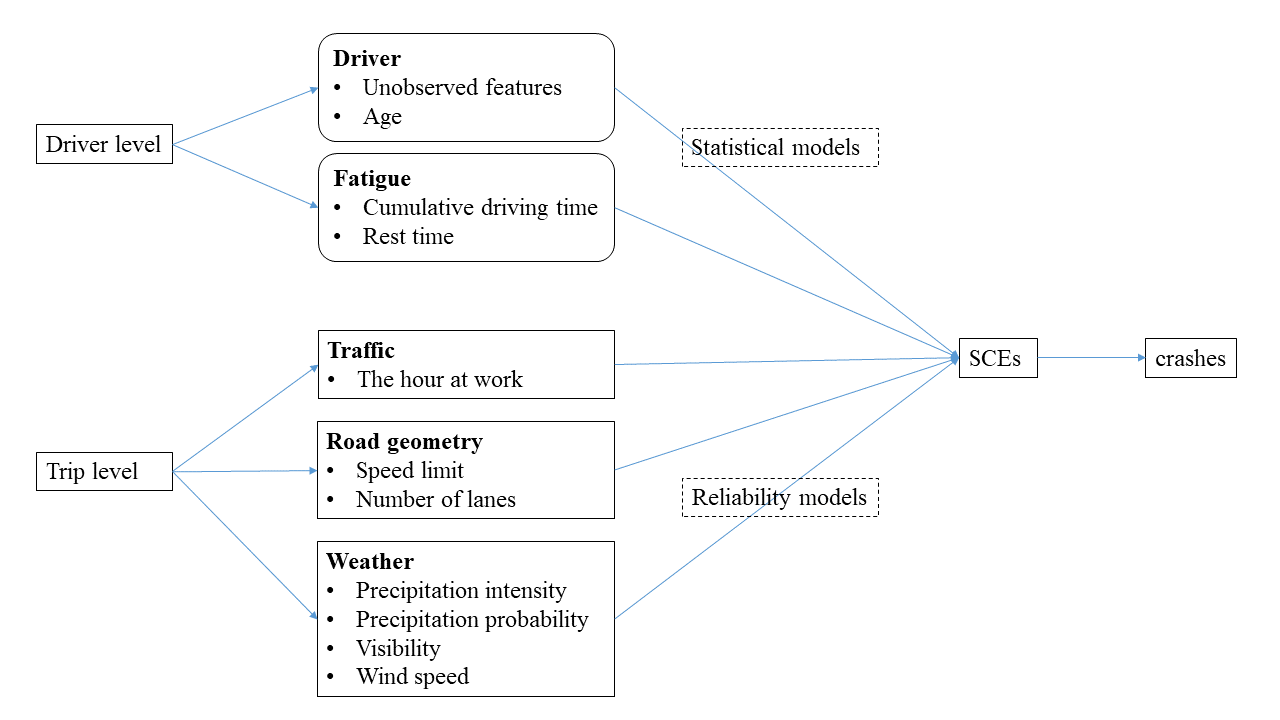
\includegraphics[width=\linewidth]{figs/conceptual_model} 

}

\caption{Conceptual model. SCEs represent safety critical events.}\label{fig:conceptmodel}
\end{figure}

\hypertarget{research-aims}{%
\section{Research aims}\label{research-aims}}

\hl{Describes the research problems to be addressed and why these are important issues.}

The overarching goal of this proposed study is to

\begin{enumerate}
\def\labelenumi{\arabic{enumi}.}
\item
  \textbf{Aim1}: to examine the association between truck crashes and critical events using a Gamma-Poisson regression.
\item
  \textbf{Aim2}: to construct three scalable Bayesian hierarchical models for SCEs: logistic regression, Poisson regression, and non-homogeneous Poisson process.
\item
  \textbf{Aim3}: to propose an innovative reliability model that accounts for both within shift cumulative driving time and within-shift between-trip rest time.
\end{enumerate}

\textbf{Gaps in literature}

\begin{itemize}
\tightlist
\item
  A focus on crashes instead of precursors of crashes
\item
  A focus on road segments rather than drivers
\item
  A focus on case-control comparison given the rareness of truck crashes rather than rates
\item
  A focus on small-scale data
\item
  A focus on traditional statistical models instead of recurrent events models
\end{itemize}

\hypertarget{methods}{%
\chapter{METHODS}\label{methods}}

\hypertarget{data-sources}{%
\section{Data sources}\label{data-sources}}

\hypertarget{real-time-ping}{%
\subsection{Real-time ping}\label{real-time-ping}}

The J.B. Hunt Transport Services, a commercial trucking and transportation company in the United States, will provid me real-time ping data generated between April 1st, 2015 and March 29th, 2016. During this time, a small device was installed in each of their truck, which will ping irregularly (typically every 2-10 minutes). Each ping will collect real-time data on the vehicle number, date and time, latitude, longitude, driver identification number (ID), and speed at that second. The driver ID is de-identified and no real driver names will be involved. In total, there are 1,494,678,173 pings.

\hypertarget{truck-crashes-and-sces}{%
\subsection{Truck crashes and SCEs}\label{truck-crashes-and-sces}}

Real-time time-stamped SCEs and associated GPS locations for all trucks were collected by the truck company and accessible to me as outcome variables. Three types of critical events were recorded:

\begin{enumerate}
\def\labelenumi{\arabic{enumi}.}
\tightlist
\item
  Hard brake
\item
  Headway
\item
  Rolling stability
\end{enumerate}

Once some thresholds with regard to the driving behavior were met, the sensor will be automatically triggered and the information of these SCEs (latitude, longitude, speed, driver ID) will be recorded.

\hypertarget{driver-demographics}{%
\subsection{Driver demographics}\label{driver-demographics}}

A table that includes the birth date of each driver will be provided by the J.B. Hunt Transport Services. The age of the driver can be calculated from this table and merged back to the trips, shifts, and crashes tables via a common unique driver ID.

\hypertarget{weather-data-from-the-dark-sky-api}{%
\subsection{\texorpdfstring{Weather data from the \texttt{Dark\ Sky\ API}}{Weather data from the Dark Sky API}}\label{weather-data-from-the-dark-sky-api}}

Weather variables, including \emph{precipitation intensity}, \emph{precipitation probability}, \emph{wind speed}, and \emph{visibility}, will be retrieved from the \texttt{Dark\ Sky\ API}.
The \texttt{Dark\ Sky\ API} allows the users to query historic minute-by-minute weather data anywhere on the globe (The Dark Sky Company, LLC, \protect\hyperlink{ref-darksky}{2019}).
According to the official document, the \texttt{Dark\ Sky\ API} is supported by a wide range of weather data sources, which are aggregated together to provide the most precise weather data possible for a given location (The Dark Sky API, \protect\hyperlink{ref-darkskyds}{2019}).
Among several different weather data providers I tested, the \texttt{Dark\ Sky\ API} provides the most accurate and complete weather variables.

To reduce the cost of querying weather data, we will focus on 496 drivers conducting regional work, which generated around the 13 million real-time ping data. These latitude and longitude coordinates will be rounded to two decimal places, which are worth up to 1.1 kilometers.
We will also round the time to the nearest hour and ignore those stopping pings.
This reduction algorithm will scaled the original 13 million real-time ping data down to around five million unique latitude-longitude-date-time combinations.
We will use the R package \texttt{darksky} to obtain weather variables for these reduced give million unique combinations (Rudis, \protect\hyperlink{ref-hrbrmstr}{2018}).
The weather data for these combinations will then be merged back to the original ping data.
A minimal example of R code to retrieve weather data from the DarkSky API can be found in Appendix \ref{weatherdat}.

\hypertarget{road-geometry-data-from-the-openstreetmap}{%
\subsection{\texorpdfstring{Road geometry data from the \texttt{OpenStreetMap}}{Road geometry data from the OpenStreetMap}}\label{road-geometry-data-from-the-openstreetmap}}

Two road geometry variables for the 496 regional truck drivers will be queried from the \texttt{OpenStreetMap} (OSM) project: \emph{speed limits} and \emph{the number of lanes}.
The OSM data are collaboratively collected by over two million registered users via manual survey, GPS devices, aerial photography, and other open-access sources (Wikipedia contributors, \protect\hyperlink{ref-wikiOSM}{2019}).
The OpenStreetMap Foundation supports a website to make the data freely available to the public under the Open Database License.

We will query the speed limits and the number of lanes by specifying a bounding box by defining a center point, as well as the width and height in meters in the \texttt{center\_bbox()} function available from the \texttt{osmar} R package (Eugster and Schlesinger, \protect\hyperlink{ref-eugster2013osmar}{2013}).
We will use real-time longitudes and latitudes as the center point and defined a \(100\times100\) meters box to retrieve the two variables.
If the \(100\times100\) meters box is too small to have any road geometry data, we will expand the box to \(500\times500\) and then \(1000\times1000\) to obtain geometry data.
If the OSM API returned data from multiple geometry structures, we will take the mean of the returned values as the output.
The R code to retrieve road geometry data can be found in Appendix \ref{roadgeometry}.

\hypertarget{data-aggregation-and-merging}{%
\section{Data aggregation and merging}\label{data-aggregation-and-merging}}

\begin{figure}[ht]

{\centering 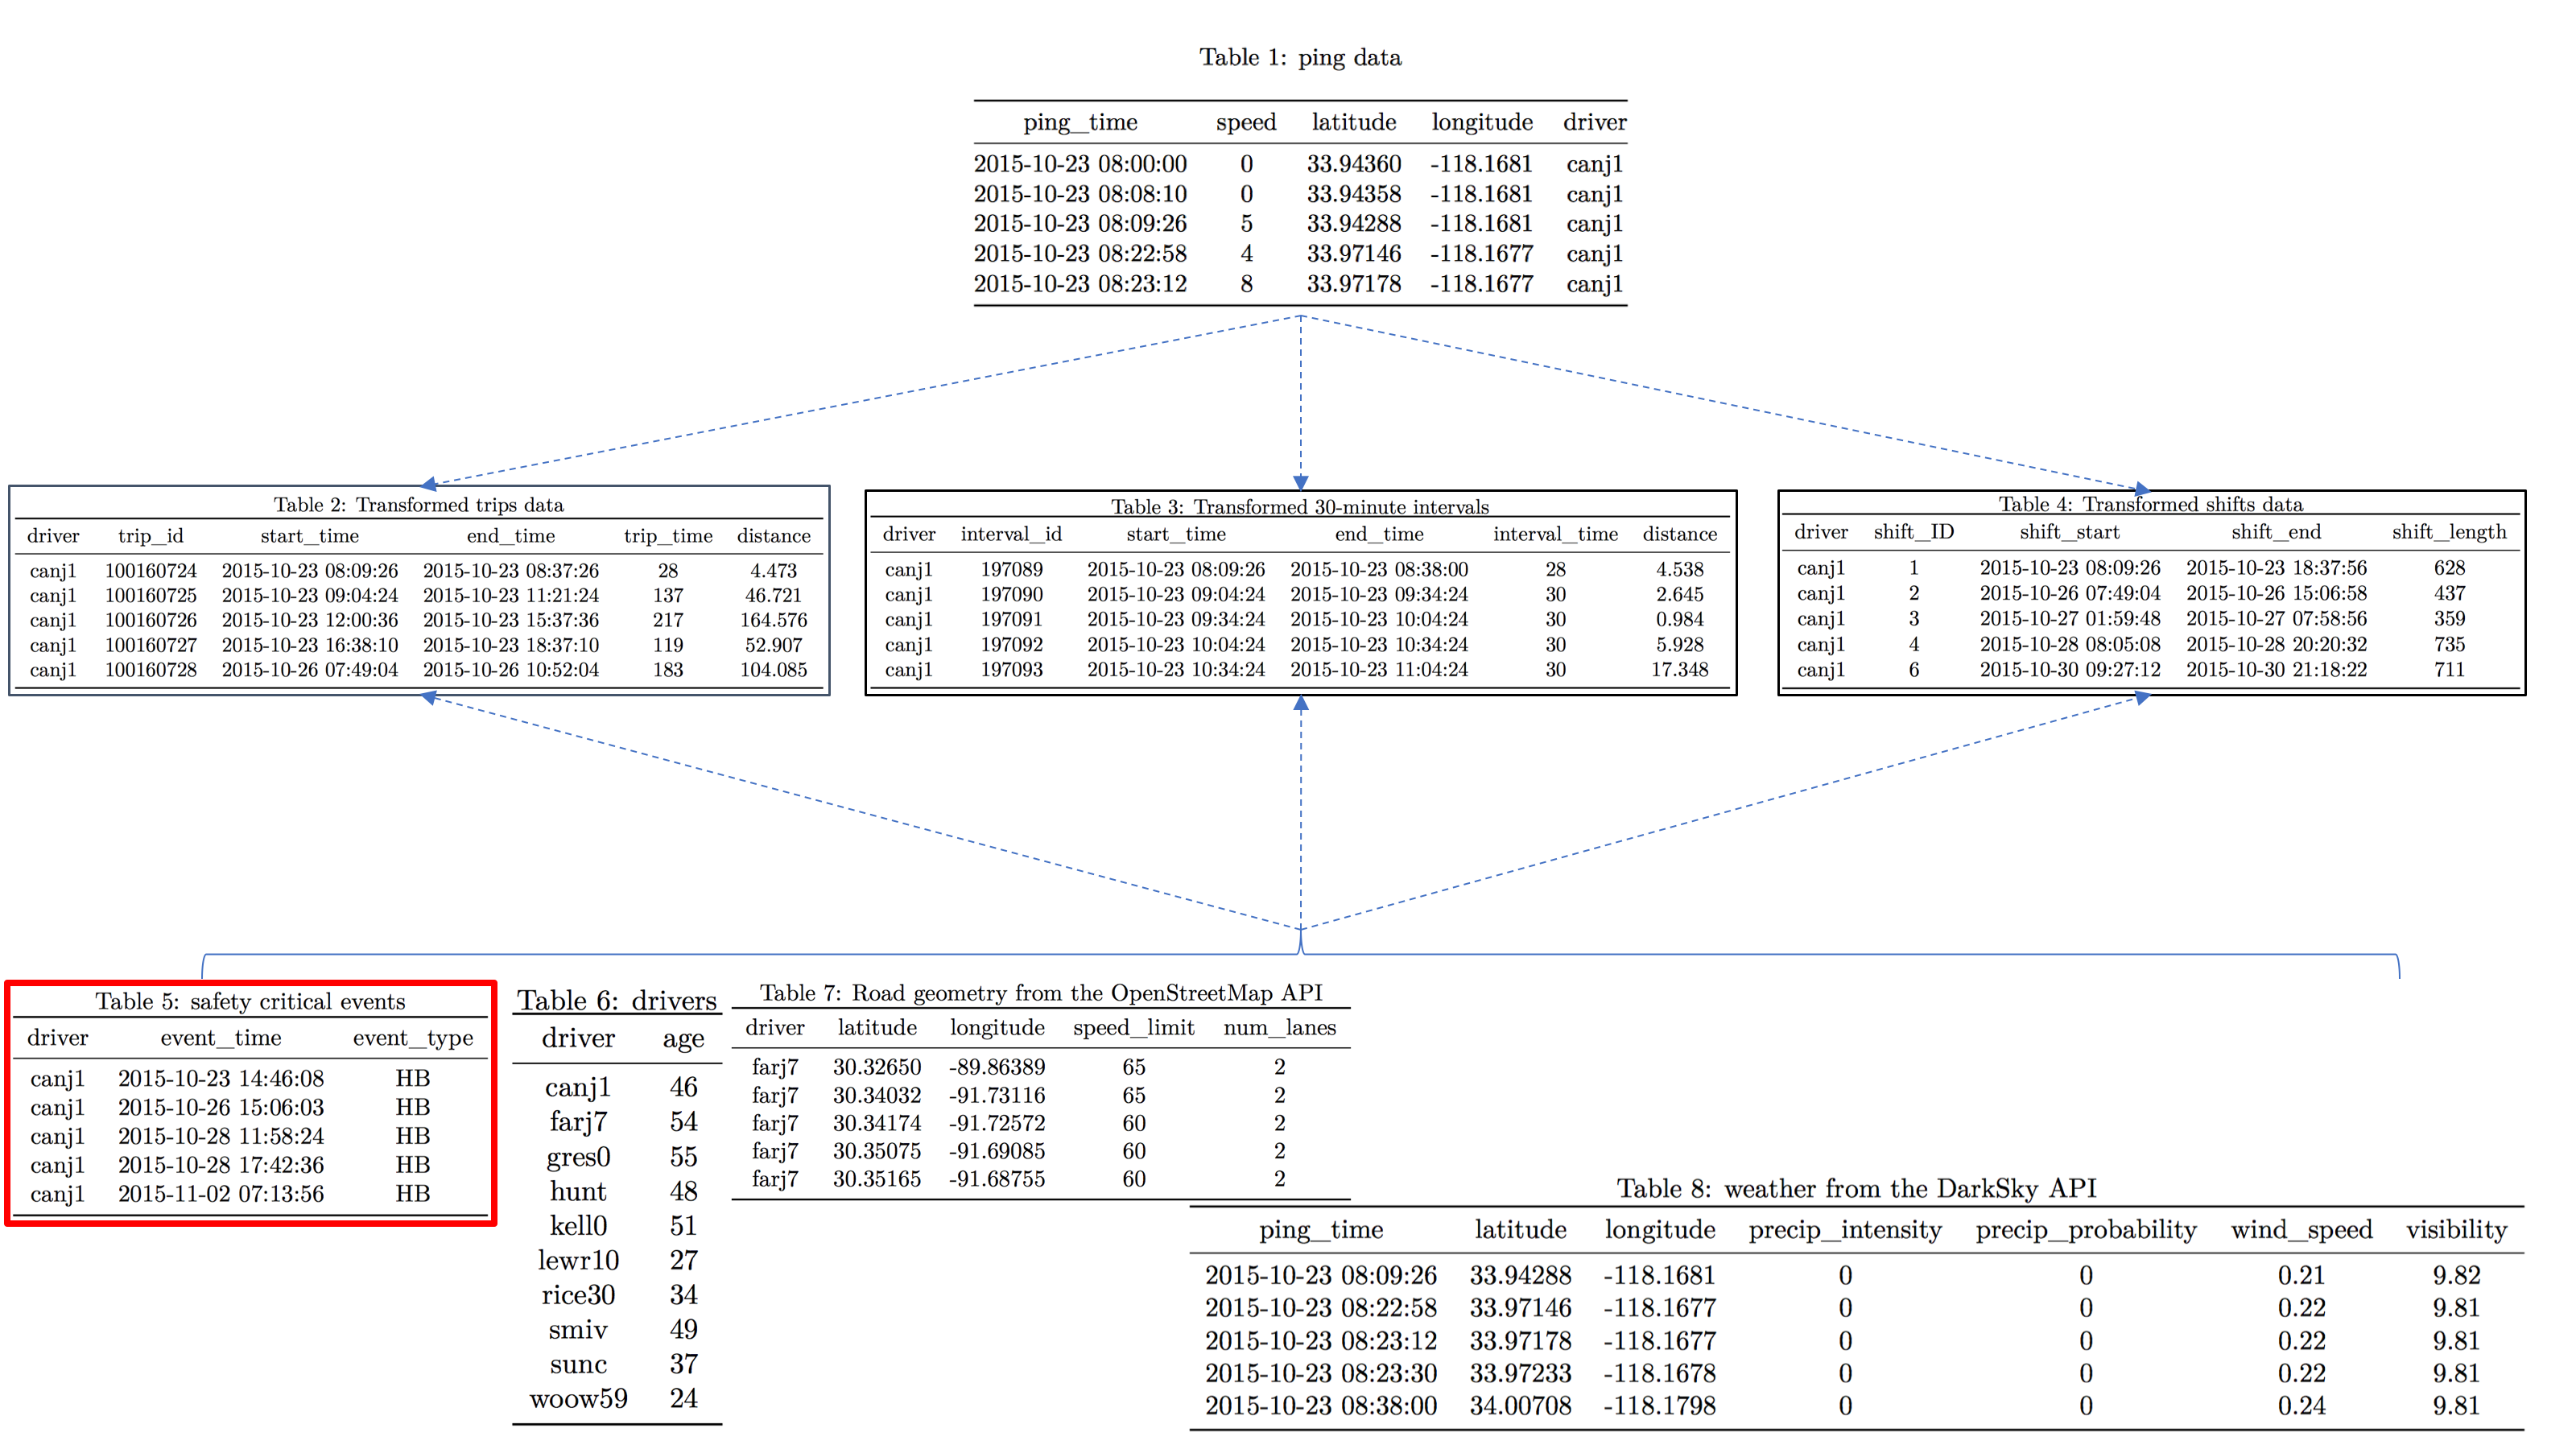
\includegraphics[width=\linewidth]{figs/Data_merging} 

}

\caption{Flow chart of data aggregation and merging}\label{fig:unnamed-chunk-1}
\end{figure}

\hypertarget{analytical-plan-for-aim-1}{%
\section{Analytical Plan for Aim 1}\label{analytical-plan-for-aim-1}}

The first aim seeks to determine the association between the rate of crashes and the rate of SCEs at the level of drivers. The cohort will be all drivers with at more than 100 pings. Drivers with less than 100 real-time pings will be recognized as potential outliers and excluded from analysis.

\hypertarget{data-reduction}{%
\subsection{Data reduction}\label{data-reduction}}

In order to make the MCMC estimation for Bayesian models tractable, I will use the following data reduction algorithms to aggregate real-time ping data to \emph{trips} and \emph{shifts}:

\begin{itemize}
\tightlist
\item
  For each of the truck drivers, if the real-time ping data showed that the truck was not moving for more than 20 minutes, the ping data will be separated into two different \emph{trips}.
\item
  These trips data will be further divided into different \emph{shifts} if the specific driver was not moving for eight hours.
\end{itemize}

Therefore, a \emph{trip} is defined as a continuous period of driving without stopping for more than 20 minutes. a \emph{shift} is defined as a long period of driving without stopping for more than 8 hours.

\hypertarget{outcome-and-predictor-variables}{%
\subsection{Outcome and predictor variables}\label{outcome-and-predictor-variables}}

The outcome variable will be the number of crashes for each driver. The primary independent variable will be the number of SCEs per 10,000 miles. These SCEs will be further decomposed into the number of hard brakes, headways, and rolling stability per 10,000 miles in similar analysis. The covariates will be the total miles driven, the percent of night driving, and the age of the drivers.

\hypertarget{statistical-models}{%
\subsection{Statistical models}\label{statistical-models}}

Since the outcome variable is a count variable, a Poisson model or a negative binomial model is a natural choice for this type of outcome variable (Lord and Mannering, \protect\hyperlink{ref-lord2010statistical}{2010}). However, these two models are less likely to fully account for the variance across drivers. Therefore, I propose to use a Gamma-Poisson model to examine the association between crashes and SCEs. Here is how the proposed Gamma-Poisson model will be implemented:

Let us assume that:
\[
\begin{aligned}
\lambda & \sim \text{Gamma}(\alpha, \beta)\\
X|\lambda & \sim \text{Poisson}(\lambda)\\
\end{aligned}
\]
Then we have:
\[X \sim \text{Gamma-Poisson}(\alpha, \beta)\]
The Gamma-Poisson distribution is a \(\alpha\)-parameter distribution, with the \(\alpha\) as a measure of overdispersion. The Gamma-Poisson distribution has the probability mass function of:
\[f(x) = \frac{\Gamma(x + \beta)\alpha^x}{\Gamma(\beta)(1 + \alpha)^{\beta + x}x!}, \quad x = 0, 1, 2, \dots\]

The mean and variance of a Gamma-Poisson distribution are:
\[
\begin{aligned}
E(X) & = \alpha\beta \\
V(X) & = \alpha\beta + \alpha^2\beta\\
     & = \alpha\beta(1 + \alpha)
\end{aligned}
\]

The log-linear Gamma-Poisson model will be specified as:
\[
\log\beta = \mathbf{X\gamma} - \log m,
\]
where \(\mathbf{X}\) is the predictor variables matrix, including the percent of night driving and the age of the drivers, \(\mathbf{\gamma}\) is the associated \(2*1\) parameter vector, \(m\) is the total miles driven as an offset term in the Poisson distribution, and \(\alpha\) is a fixed overdispersion parameter that does not depend on any covariates.

All data reduction, cleaning, and statistical analysis will be done on the RStudio Server on the Ohio Supercomputer Center (OSC). The OSC provides high performance computing resources and expertise to academic researchers (Center, \protect\hyperlink{ref-OSC1987}{1987}). The Bayesian statistical models will be conducted using the \texttt{rstan} package in R 3.5.1 (R Core Team, \protect\hyperlink{ref-Rcitation}{2018}; Stan Development Team, \protect\hyperlink{ref-rstancitation}{2018}).

\hypertarget{analytical-plan-for-aim-2}{%
\section{Analytical Plan for Aim 2}\label{analytical-plan-for-aim-2}}

The purpose of aim 2 is to develop three hierarchical Bayesian statistical and reliability models for the SCEs of truck drivers. Vehicle drivers will be viewed as the sampling unit. The workflow is to sample a certain number of drivers from a population of drivers, observe their driving trips or shifts for a specific period, then compare the safety events with non-events, and make conclusions on risk factors associated with these safety events. Bayesian hierarchical logistic regression, Poisson regression, and NHPP that accounts for both driver-level variation and trip-level variation will be used.

\hypertarget{data-aggregation}{%
\subsection{Data aggregation}\label{data-aggregation}}

\hypertarget{logistic-regression}{%
\subsection{Logistic regression}\label{logistic-regression}}

Here the probability of a critical event occurred will be modeled using a Bayesian hierarchical logistic regression. I will categorize the number of safety events during a trip into a binary variable \(Y_{i, d}\) of either 0 or 1, where 0 indicates that no critical event occurred during that trip while 1 indicates that at least 1 critical event occurred during the trip.
\[
\begin{split}
Y_{i} &\sim \text{Bernoulli}(p_{i})\\
\log\frac{p_{i}}{1-p_{i}} &= \beta_{0, d(i)} + \beta_{1, d(i)} \cdot \text{CT}_i + \sum_{j=1}^{J} x_{ij}\beta_j\\
\beta_{0, d} &\sim \text{i.i.d. } N(\mu_0, \sigma_0^2), \quad d = 1, 2, \cdots, D\\
\beta_{1, d} &\sim \text{i.i.d. } N(\mu_1, \sigma_1^2), \quad d = 1, 2, \cdots, D
\label{eq:hierarchicallogit}
\end{split}
\]

We assume that the drivers are random effects, and we assume exchangeable priors of the form
\[
\beta_{0, d(1)}, \beta_{0, d(2)}, \ldots , \beta_{0, d(n)} \sim \text{i.i.d.} N(\mu_0,\sigma_0^2)
\]
and
\[
\beta_{1, d(1)}, \beta_{1, d(2)}, \ldots , \beta_{1, d(n)} \sim \text{i.i.d.} N(\mu_1,\sigma_1^2)
\]
The parameters \(\mu_0, \sigma_0, \mu_1\), and \(\sigma_1\) are hyperparameters with priors. Since we do not have much prior knowledge on the hyperparameters, we assigned diffuse priors for these hyperparameters.
\[
\begin{split}
Y_{i} &\sim \text{Bernoulli}(p_{i})\\
\log\frac{p_{i}}{1-p_{i}} &= \beta_{0, d(i)} + \beta_{1, d(i)} \cdot \text{CT}_i + \sum_{j=1}^{J} x_{ij}\beta_j\\
\beta_{0, d} &\sim \text{i.i.d. } N(\mu_0, \sigma_0^2), \quad d = 1, 2, \cdots, D\\
\beta_{1, d} &\sim \text{i.i.d. } N(\mu_1, \sigma_1^2), \quad d = 1, 2, \cdots, D
\label{eq:priors}
\end{split}
\]
Since \(\mu_0\) and \(\mu_1\) can be any real number, so we assigned two normal distributions with mean of 0 and standard deviation of 10 as the priors for these two hyperparameters. In comparison, \(\sigma_0\) and \(\sigma_1\) must be strictly positive, so we assigned GAMMA\((1, 1)\) with wide distribution on positive real numbers as their priors.

\hypertarget{poisson-regression}{%
\subsection{Poisson regression}\label{poisson-regression}}

Since logistic regression ignores the intensity of the critical events with any number greater than 0 categorized into 1, I adopt a Bayesian hierarchical Poisson regression to model the effect of cumulative driving time on the occurrence of critical events. Each driver has a random intercept and a random slope on cumulative driving time.
\[
\begin{split}
Y_{i}  & \sim \text{Poisson}(T_i\cdot\lambda_i)\\
\log\lambda_{i} & =\beta_{0, d(i)} + \beta_{1, d(i)} \cdot \text{CT}_i + \sum_{j=1}^{J} x_{ij}\beta_j\\
\beta_{0, d} &\sim \text{i.i.d. } N(\mu_0, \sigma_0^2), \quad d = 1, 2, \cdots, D\\
\beta_{1, d} &\sim \text{i.i.d. } N(\mu_1, \sigma_1^2), \quad d = 1, 2, \cdots, D
\label{eq:hierarchicalpoisson}
\end{split}
\]
Where N is the number of critical events for driver \(d(i)\) in time interval \(j\), and it has a Poisson distribution with parameter \(\lambda\). The other variables are identical as those described in Equation .

\hypertarget{non-homogeneous-poisson-process-nhpp}{%
\subsection{Non-homogeneous Poisson process (NHPP)}\label{non-homogeneous-poisson-process-nhpp}}

\begin{figure}[ht]

{\centering 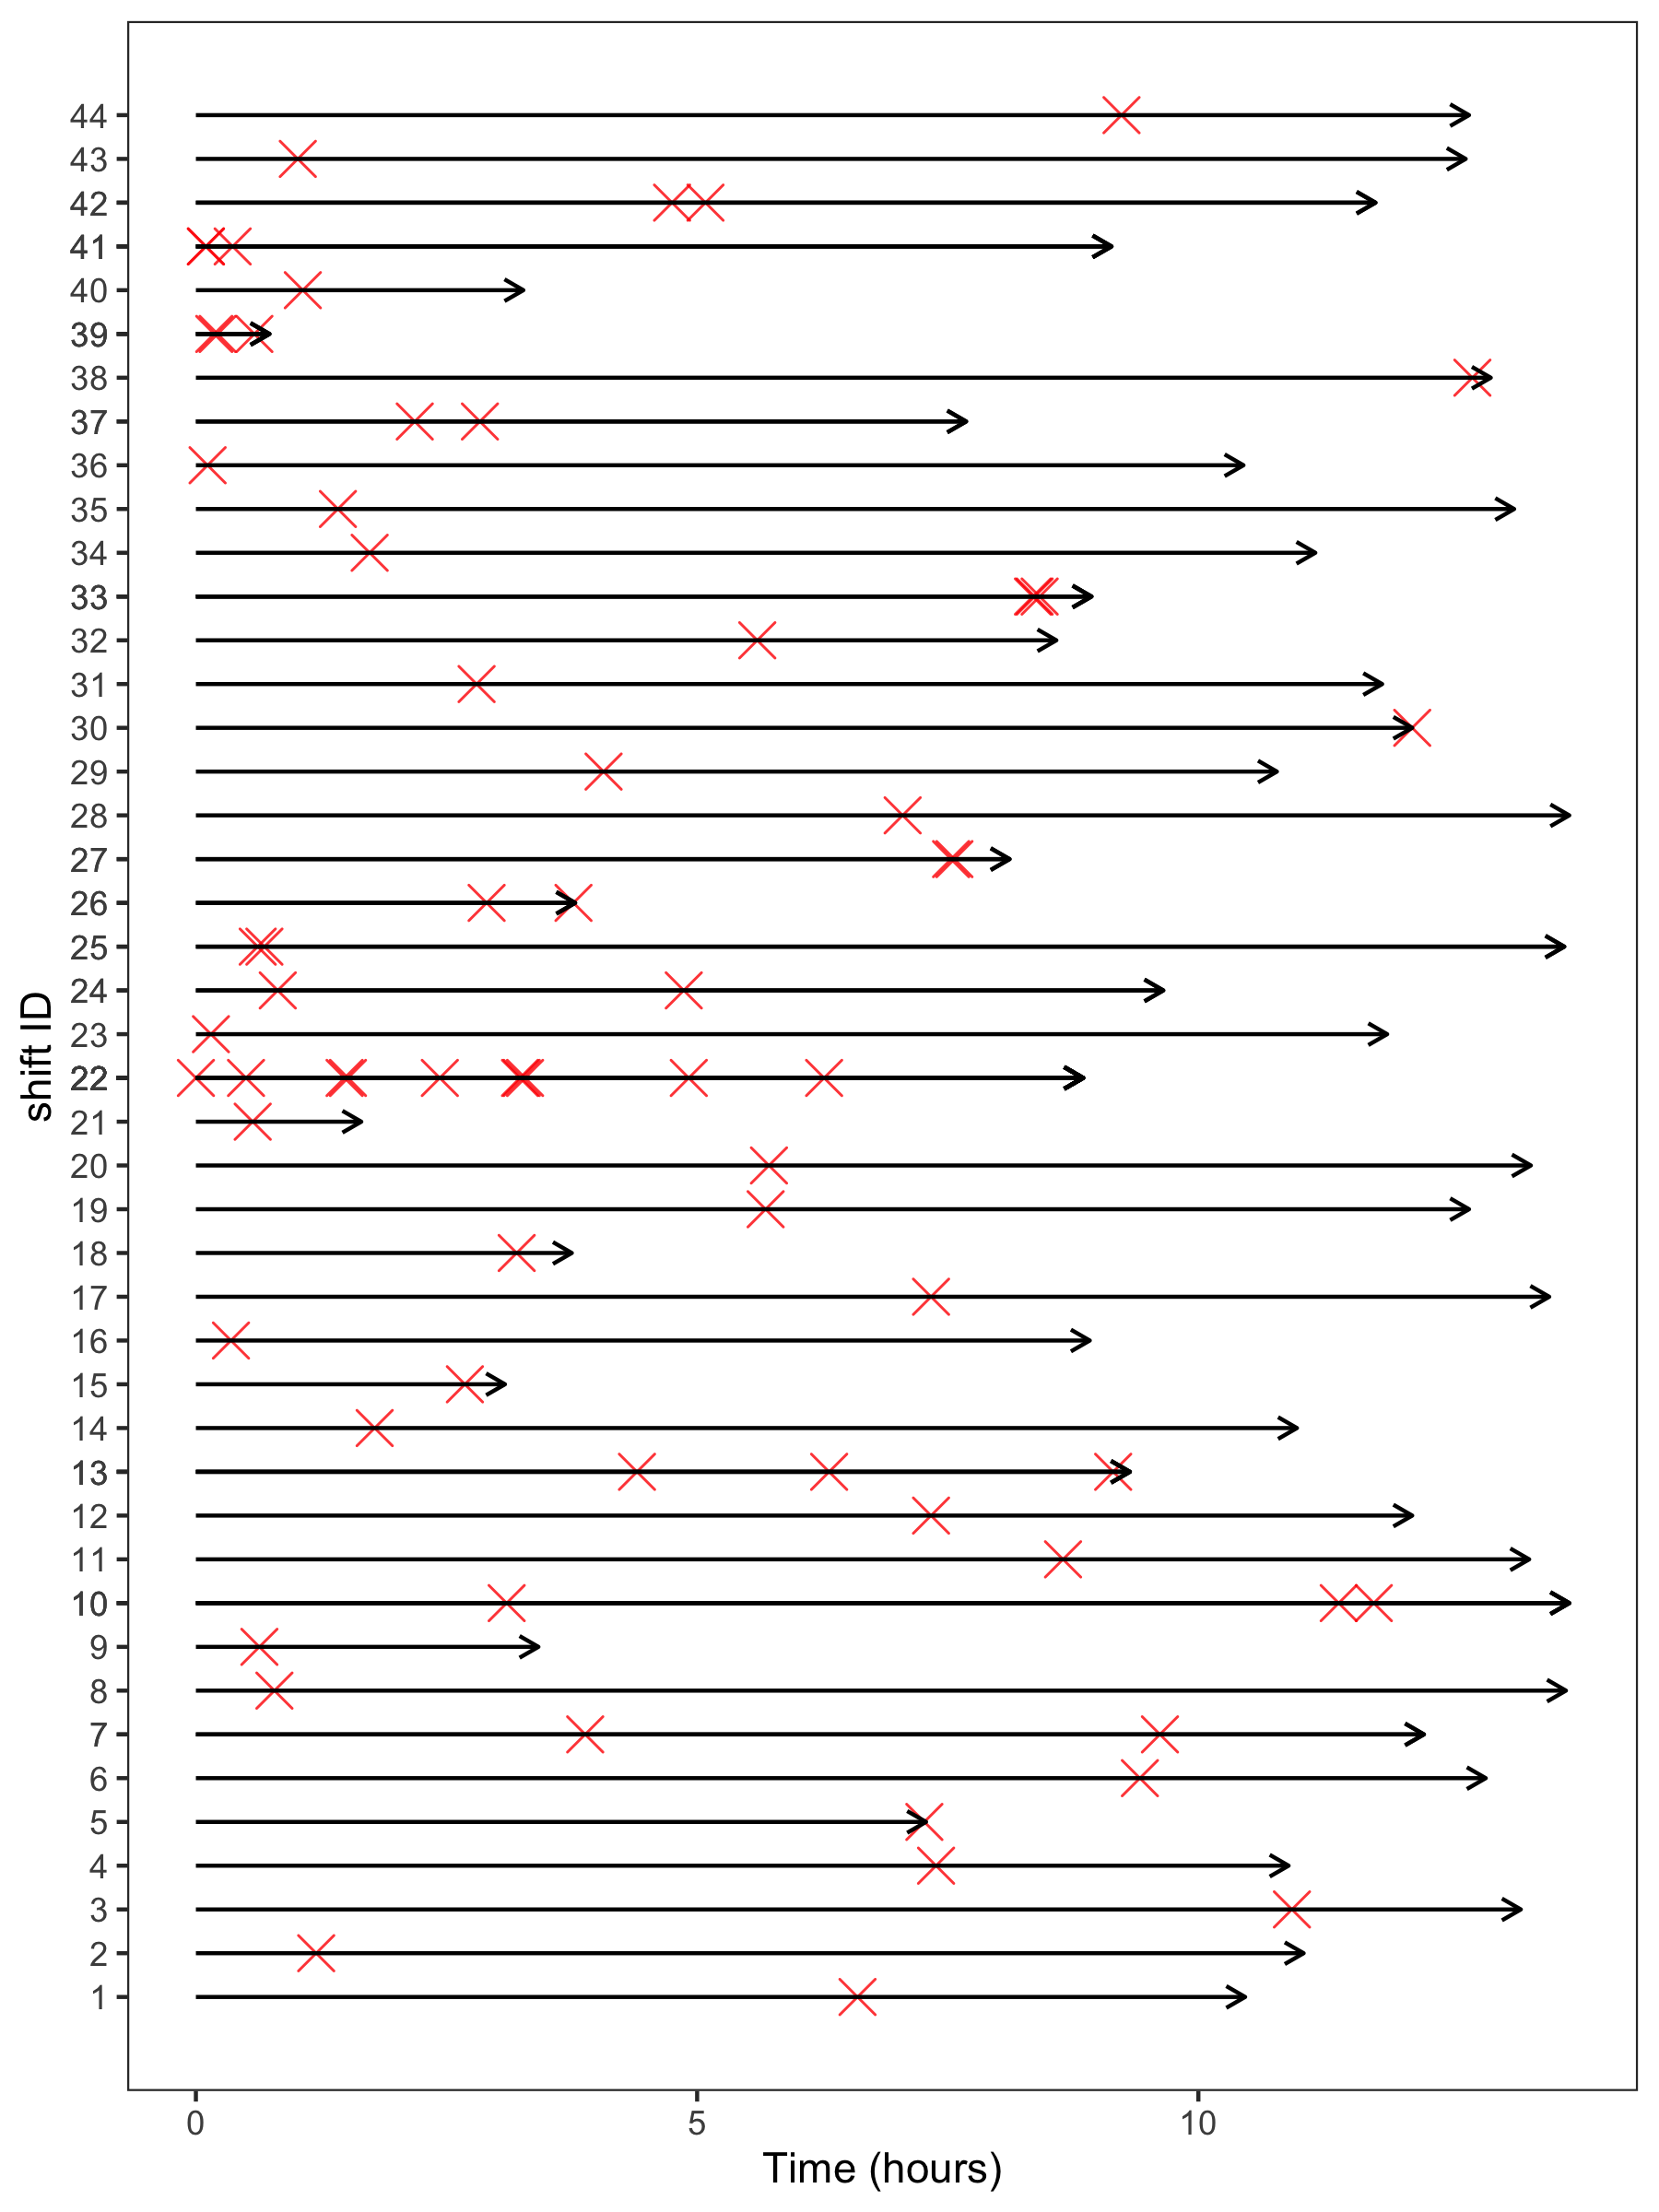
\includegraphics[width=0.5\linewidth]{figs/NHPP_arrow_plot} 

}

\caption{An arrow plot of time to SCEs in each shift}\label{fig:arrowplot}
\end{figure}

A point process is a stochastic model which describes the occurrence of events in a given period (Rigdon and Basu, \protect\hyperlink{ref-rigdon2000statistical}{2000}). The mean function of a point process is \(\Lambda(t) = E(N(t))\), where \(\Lambda(t)\) is the expected number of failures through time \(t\). Two notations that are important in reliability models are \emph{Rate of Occurence of Failures (ROCOF)} and \emph{Intensity function}.

\begin{enumerate}
\def\labelenumi{\arabic{enumi}.}
\item
  \emph{ROCOF}: When the mean function \(\Lambda(t)\) is differentiable, the ROCOF is:
  \[\mu(t) = \frac{d}{dt}\Lambda(t)\]
  The ROCOF can be interpreted as the instantaneous rate of change in the expected number of failures.
\item
  \emph{Intensity function}: The intensity function of a point process is
  \[\lambda(t) = \lim_{\Delta t \rightarrow 0}\frac{P(N(t, t+\Delta t] \geq 1)}{\Delta t}\]
\end{enumerate}

When there is no simultaneous events, ROCOF is the same as intensity function.

\emph{Nonhomogeneous Poisson Process (NHPP)}: The NHPP is a Poisson process whose intensity function is non-constant. The Power law process (PLP) is a special case of a NHPP when the intensity function of a NHPP is:
\[\lambda(t) = \frac{\beta}{\theta}\bigg(\frac{t}{\theta}\bigg)^{\beta-1}\],
Where \(\beta > 0\) and \(\theta > 0\), the process is called the power law process (PLP).

Therefore, the mean function \(\Lambda(t)\) is the integral of the intensity function:
\[\Lambda(t) = \int_0^t \lambda(t)dt = \int_0^t \frac{\beta}{\theta}\bigg(\frac{t}{\theta}\bigg)^{\beta-1} = \bigg(\frac{t}{\theta}\bigg)^{\beta}\].

There are two forms of truncation in a NHPP:

\begin{enumerate}
\def\labelenumi{\arabic{enumi}.}
\tightlist
\item
  \textbf{Failure truncation}: When testing stops after a predetermined number of failures, the data are said to be failure truncated.
\item
  \textbf{Time truncation}: Data are said to be time truncated when testing stops at a predetermined time \(t\).
\end{enumerate}

In a time truncated case, the joint likelihood function for \(f(n, t_1, t_2, \cdots, t_n)\) is (the prove can be found in the Appendix):
\begin{equation}\label{pdftau}
\begin{aligned}
f(n, t_1, t_2, \cdots, t_n) & = f(n)f(t_1, t_2, \cdots, t_n|n)\\
& = \frac{e^{-\int_0^\tau \lambda(u)du}[\int_0^\tau \lambda(u)du]^n}{n!}n!\frac{\prod_{i=1}^n\lambda(t_i)}{[\Lambda(\tau)]^n}\\
& = \Big(\prod_{i=1}^n\lambda(t_i) \Big)e^{-\int_0^\tau \lambda(u)du}\\
& = \Big(\prod_{i=1}^n\frac{\beta}{\theta}(\frac{t_i}{\theta})^{\beta - 1} \Big)e^{-(\tau/\theta)^\beta},\\ 
n & = 0, 1, 2, \cdots, \quad  0 < t_1 < t_2 < \cdots < t_n
\end{aligned}
\end{equation}

The log likelihood function \(l\) is then:
\begin{equation}\label{logtau}
\begin{aligned}
l & = \log \Bigg(\Big(\prod_{i=1}^n\frac{\beta}{\theta}(\frac{t_i}{\theta})^{\beta - 1}\Big)e^{-(\tau/\theta)^\beta}\Bigg)\\
& = \sum_{i=1}^n\log\Big(\frac{\beta}{\theta}(\frac{t_i}{\theta})^{\beta - 1}\Big) - (\frac{\tau}{\theta})^\beta\\
& = n\log\beta - n\beta\log\theta + (\beta - 1)\bigg(\sum_{i=1}^n\log t_i\bigg) - \Big(\frac{\tau}{\theta}\Big)^\beta
\end{aligned}
\end{equation}

Despite Poisson regression consider the frequency of SCEs in a given interval, it assumes that the intensity of events is a constant, which may not be true in real-life transportation practice. Here we presented a reliability model, a non-homogeneous Poisson process (NHPP) with a power law process (PLP) based on the merged shifts data set. we aim to answer if SCEs occurred more frequently at early stages of shifts, towards the end of shifts, or does not show significant patterns.

Let \(T_{d, s, i}\) denote the time to the \(d\)-th driver's \(s\)-th shift's \(i\)-th critical event. The total number critical events of \(d\)-th driver's \(s\)-th shift is \(n_{d,s}\). The ranges of these notations are:

\begin{itemize}
\tightlist
\item
  \(i = 1, 2, \cdots, n_{d, S_d}\),
\item
  \(s = 1, 2, \cdots, S_d\),
\item
  \(d = 1, 2, \cdots, D\).
\end{itemize}

We assumes that the times of critical events within the \(d\)-th driver's \(s\)-th shift were generated from a PLP, with a fixed shape parameter \(\beta\) and varying scale parameters \(\theta_{d, s}\) across drivers \(d\) and shifts \(s\). In a PLP, the intensity function of the NHPP is \(\lambda(t) \frac{\beta}{\theta}(\frac{t}{\theta})^{\beta-1}\). The model is described in Equation\textasciitilde{}\ref{eq:nhpp}.
\begin{equation}\label{eq:nhpp}
\begin{aligned}
  T_{d, s, 1}, T_{d, s, 2}, \cdots , T_{d, s, n_{d, s}} & \sim \text{PLP}(\beta, \theta_{d, s})\\
  \beta & \sim \text{Gamma}(1, 1)\\
  \log\theta_{d, s} &= \gamma_{0d} + \gamma_{1}x_{d, s, 1} + \gamma_{2}x_{d, s, 2} + \cdots + \gamma_{k}x_{d, s, k}\\
  \gamma_{01}, \gamma_{02}, \cdots, \gamma_{0D} & \sim \text{i.i.d. }N(\mu_0, \sigma_0^2)\\
  \gamma_1, \gamma_2, \cdots, \gamma_k & \sim \text{i.i.d. }N(0, 10^2)\\
  \mu_0 &\sim N(0, 10^2) \\
  \sigma_0 &\sim \text{Gamma}(1, 1)
\end{aligned}
\end{equation}
The shape parameter \(\beta\) shows the reliability changes of drivers. When \(\beta > 1\), the intensity function \(\lambda(t)\) is increasing, the reliability of drivers is decreasing, and SCEs are becoming more frequent; when \(\beta < 1\), the intensity function \(\lambda(t)\) is decreasing, the reliability of drivers is increasing, and SCEs are becoming less frequent; when \(\beta = 1\), the NHPP is simplified as a homogeneous Poisson process with the intensity of \(1/\theta\). The \(\theta_{d, s}\) is a scale parameter that does not reflect reliability changes.

\hypertarget{analytical-plan-for-aim-3}{%
\section{Analytical Plan for Aim 3}\label{analytical-plan-for-aim-3}}

Aim 3 seeks to innovate the NHPP proposed in Aim 2 by accounting for the rest time within a shift. One more parameter, the percent of reliability recovery during a break within a shift, will be estimated for in this model.

Black and Rigdon (\protect\hyperlink{ref-black1996statistical}{1996}) gives an alternative plan for achieving Aim 3.

\hypertarget{the-probable-content}{%
\chapter{THE PROBABLE CONTENT}\label{the-probable-content}}

The contents will follow the standard format for a traditional dissertation, as per guidelines set by the College for Public Health and Social Justice and Saint Louis University's Office of Graduate Education.

Chapter 1: Introduction: The problem

\begin{enumerate}
\def\labelenumi{\arabic{enumi}.}
\tightlist
\item
  Transportation safety
\item
  Truck safety
\item
  Modern Truck Safety Studies
\end{enumerate}

Chapter 2: Literature review

\begin{enumerate}
\def\labelenumi{\arabic{enumi}.}
\tightlist
\item
  Naturalistic driving Study (NDS)
\item
  Safety-critical events (SCEs)
\item
  Crashes and SCEs
\item
  Risk factors for traffic safety
\item
  Predictive models
  a. Overview
  b. Bayesian models
  c. Hierarchical models
  d. Markov chain Monte Carlo (MCMC)
\item
  Scalable Bayesian models
  a. Hamiltonian Monte Carlo (HMC)
  b. Subsampling MCMC
\end{enumerate}

Chapter 3: Aim 1 - truck crashes and critical events

\begin{enumerate}
\def\labelenumi{\arabic{enumi}.}
\tightlist
\item
  Introduction
\item
  Data sources
\item
  Methods
\item
  Results
  a. A simulation study on Gamma-Poisson models
  b. Real-world application on all SCEs
  c. Real-world application on different types of SCEs
\item
  Discussion
\end{enumerate}

Chapter 4: Aim 2 - Bayesian hierarchical models for SCEs

\begin{enumerate}
\def\labelenumi{\arabic{enumi}.}
\tightlist
\item
  Introduction
\item
  Data sources
\item
  Methods
  a. Logistic regression
  b. Poisson regression
  c. Non-homogeneous Poisson process (NHPP)
\item
  Results
  a. Logistic regression
  b. Poisson regression
  c. NHPP

  \begin{enumerate}
  \def\labelenumii{\roman{enumii}.}
  \tightlist
  \item
    A simulation study on NHPP
  \item
    Real-world application on NHPP
  \end{enumerate}
\item
  Discussion
\end{enumerate}

Chapter 5: Aim 3 - an innovation on NHPP to account for within shift rest time

\begin{enumerate}
\def\labelenumi{\arabic{enumi}.}
\tightlist
\item
  Introduction
\item
  Data sources
\item
  Methods
\item
  Results
  a. A simulation study on this new method
  b. Real-world application on this new method
  c. Real-world application on this new method stratified by SCE types
\item
  Discussion
\end{enumerate}

Chapter 6: Discussion

\begin{enumerate}
\def\labelenumi{\arabic{enumi}.}
\tightlist
\item
  Conclusion
\item
  Strengths and limitation
\item
  Future research
\end{enumerate}

\hypertarget{discussion}{%
\chapter{DISCUSSION}\label{discussion}}

--\textgreater{}

\singlespacing

\chapter*{\markboth{APPENDIX}{APPENDIX}{APPENDIX}}
\addcontentsline{toc}{chapter}{APPENDIX}

\hypertarget{weatherdat}{%
\section*{Query weather data}\label{weatherdat}}
\addcontentsline{toc}{section}{Query weather data}

\begin{Shaded}
\begin{Highlighting}[]
\NormalTok{gps_sample =}\StringTok{ }
\StringTok{  }\KeywordTok{structure}\NormalTok{(}\KeywordTok{list}\NormalTok{(}
    \DataTypeTok{from_lat =} \KeywordTok{c}\NormalTok{(}\FloatTok{41.3473127}\NormalTok{, }\FloatTok{41.8189037}\NormalTok{, }\FloatTok{32.8258477}\NormalTok{, }\FloatTok{40.6776808}\NormalTok{, }
                 \FloatTok{40.2366043}\NormalTok{, }\FloatTok{41.3945561}\NormalTok{, }\FloatTok{32.6320605}\NormalTok{, }\FloatTok{40.5413856}\NormalTok{, }
                 \FloatTok{33.6287422}\NormalTok{, }\FloatTok{40.0692742}\NormalTok{, }\FloatTok{41.347986}\NormalTok{, }\FloatTok{37.7781459}\NormalTok{, }
                 \FloatTok{43.0843081}\NormalTok{, }\FloatTok{41.48026}\NormalTok{, }\FloatTok{43.495149}\NormalTok{, }\FloatTok{41.5228684}\NormalTok{, }
                 \FloatTok{41.5763081}\NormalTok{, }\FloatTok{47.6728665}\NormalTok{, }\FloatTok{41.0918361}\NormalTok{, }\FloatTok{41.1537819}\NormalTok{),}
    \DataTypeTok{from_lon =} \KeywordTok{c}\NormalTok{(}\OperatorTok{-}\FloatTok{74.2850908}\NormalTok{, }\FloatTok{-73.0835104}\NormalTok{, }\FloatTok{-97.0306677}\NormalTok{, }\FloatTok{-75.1450753}\NormalTok{,}
                 \FloatTok{-76.9367494}\NormalTok{, }\FloatTok{-72.8589916}\NormalTok{, }\FloatTok{-96.8538145}\NormalTok{, }\FloatTok{-74.8547061}\NormalTok{, }
                 \FloatTok{-113.7671634}\NormalTok{, }\FloatTok{-76.762612}\NormalTok{, }\FloatTok{-74.284785}\NormalTok{, }\FloatTok{-77.4615586}\NormalTok{, }
                 \FloatTok{-76.0977384}\NormalTok{, }\FloatTok{-73.2107541}\NormalTok{, }\FloatTok{-73.7727896}\NormalTok{, }\FloatTok{-74.0739204}\NormalTok{, }
                 \FloatTok{-88.1529175}\NormalTok{, }\FloatTok{-117.3224667}\NormalTok{, }\FloatTok{-74.1554972}\NormalTok{, }\FloatTok{-74.1887031}\NormalTok{), }
    \DataTypeTok{beg_time =} \KeywordTok{structure}\NormalTok{(}
      \KeywordTok{c}\NormalTok{(}\DecValTok{1453101738}\NormalTok{, }\DecValTok{1437508088}\NormalTok{, }\DecValTok{1436195038}\NormalTok{, }\DecValTok{1435243088}\NormalTok{, }\DecValTok{1454270680}\NormalTok{, }
        \DecValTok{1432210106}\NormalTok{, }\DecValTok{1438937772}\NormalTok{, }\DecValTok{1446486480}\NormalTok{, }\DecValTok{1450191622}\NormalTok{, }\DecValTok{1449848630}\NormalTok{, }
        \DecValTok{1457597084}\NormalTok{, }\DecValTok{1432870446}\NormalTok{, }\DecValTok{1457968284}\NormalTok{, }\DecValTok{1451298724}\NormalTok{, }\DecValTok{1431503502}\NormalTok{, }
        \DecValTok{1443416864}\NormalTok{, }\DecValTok{1438306368}\NormalTok{, }\DecValTok{1445540454}\NormalTok{, }\DecValTok{1452619392}\NormalTok{, }\DecValTok{1436091072}\NormalTok{), }
      \DataTypeTok{class =} \KeywordTok{c}\NormalTok{(}\StringTok{"POSIXct"}\NormalTok{, }\StringTok{"POSIXt"}\NormalTok{), }\DataTypeTok{tzone =} \StringTok{"UTC"}\NormalTok{)), }
    \DataTypeTok{.Names =} \KeywordTok{c}\NormalTok{(}\StringTok{"from_lat"}\NormalTok{, }\StringTok{"from_lon"}\NormalTok{, }\StringTok{"beg_time"}\NormalTok{), }
    \DataTypeTok{row.names =} \KeywordTok{c}\NormalTok{(}\OtherTok{NA}\NormalTok{, 20L), }
    \DataTypeTok{class =} \KeywordTok{c}\NormalTok{(}\StringTok{"tbl_df"}\NormalTok{, }\StringTok{"tbl"}\NormalTok{, }\StringTok{"data.frame"}\NormalTok{))}
\NormalTok{gps_sample}
\end{Highlighting}
\end{Shaded}

\begin{Shaded}
\begin{Highlighting}[]
\KeywordTok{library}\NormalTok{(darksky)}
\NormalTok{add_var =}\StringTok{ }\ControlFlowTok{function}\NormalTok{(dat)\{}
\NormalTok{  dat[,}\KeywordTok{c}\NormalTok{(}\StringTok{"time"}\NormalTok{, }\StringTok{"summary"}\NormalTok{, }\StringTok{"icon"}\NormalTok{, }\StringTok{"precipIntensity"}\NormalTok{, }
         \StringTok{"precipProbability"}\NormalTok{, }\StringTok{"temperature"}\NormalTok{, }\StringTok{"apparentTemperature"}\NormalTok{, }
         \StringTok{"dewPoint"}\NormalTok{, }\StringTok{"humidity"}\NormalTok{, }\StringTok{"pressure"}\NormalTok{, }\StringTok{"windSpeed"}\NormalTok{, }\StringTok{"windGust"}\NormalTok{, }
         \StringTok{"windBearing"}\NormalTok{, }\StringTok{"cloudCover"}\NormalTok{, }\StringTok{"visibility"}\NormalTok{)] =}\StringTok{ }\OtherTok{NA}
  \KeywordTok{return}\NormalTok{(dat)}
\NormalTok{\}}

\ControlFlowTok{for}\NormalTok{(i }\ControlFlowTok{in} \DecValTok{1}\OperatorTok{:}\KeywordTok{nrow}\NormalTok{(gps_sample))\{}
\NormalTok{  t =}\StringTok{ }\KeywordTok{get_forecast_for}\NormalTok{(gps_sample}\OperatorTok{$}\NormalTok{from_lat[i], gps_sample}\OperatorTok{$}\NormalTok{from_lon[i], }
\NormalTok{                       gps_sample}\OperatorTok{$}\NormalTok{beg_time[i])}
\NormalTok{  gps_sample}\OperatorTok{$}\NormalTok{summary[i] =}\StringTok{ }\KeywordTok{ifelse}\NormalTok{(}\KeywordTok{is.null}\NormalTok{(t[[}\DecValTok{3}\NormalTok{]]}\OperatorTok{$}\NormalTok{summary), }\OtherTok{NA}\NormalTok{, }
\NormalTok{                                 t[[}\DecValTok{3}\NormalTok{]]}\OperatorTok{$}\NormalTok{summary)}
\NormalTok{  gps_sample}\OperatorTok{$}\NormalTok{icon[i] =}\StringTok{ }\KeywordTok{ifelse}\NormalTok{(}\KeywordTok{is.null}\NormalTok{(t[[}\DecValTok{3}\NormalTok{]]}\OperatorTok{$}\NormalTok{icon), }\OtherTok{NA}\NormalTok{, t[[}\DecValTok{3}\NormalTok{]]}\OperatorTok{$}\NormalTok{icon)}
\NormalTok{  gps_sample}\OperatorTok{$}\NormalTok{precipIntensity[i] =}\StringTok{ }\KeywordTok{ifelse}\NormalTok{(}\KeywordTok{is.null}\NormalTok{(t[[}\DecValTok{3}\NormalTok{]]}\OperatorTok{$}\NormalTok{precipIntensity), }
                                         \OtherTok{NA}\NormalTok{, t[[}\DecValTok{3}\NormalTok{]]}\OperatorTok{$}\NormalTok{precipIntensity)}
\NormalTok{  gps_sample}\OperatorTok{$}\NormalTok{precipProbability[i] =}\StringTok{ }\KeywordTok{ifelse}\NormalTok{(}\KeywordTok{is.null}\NormalTok{(t[[}\DecValTok{3}\NormalTok{]]}\OperatorTok{$}\NormalTok{precipProbability), }
                                           \OtherTok{NA}\NormalTok{, t[[}\DecValTok{3}\NormalTok{]]}\OperatorTok{$}\NormalTok{precipProbability)}
\NormalTok{  gps_sample}\OperatorTok{$}\NormalTok{temperature[i] =}\StringTok{ }\KeywordTok{ifelse}\NormalTok{(}\KeywordTok{is.null}\NormalTok{(t[[}\DecValTok{3}\NormalTok{]]}\OperatorTok{$}\NormalTok{temperature), }\OtherTok{NA}\NormalTok{, }
\NormalTok{                                     t[[}\DecValTok{3}\NormalTok{]]}\OperatorTok{$}\NormalTok{temperature)}
\NormalTok{  gps_sample}\OperatorTok{$}\NormalTok{apparentTemperature[i] =}\StringTok{ }\KeywordTok{ifelse}\NormalTok{(}\KeywordTok{is.null}\NormalTok{(}
\NormalTok{    t[[}\DecValTok{3}\NormalTok{]]}\OperatorTok{$}\NormalTok{apparentTemperature), }\OtherTok{NA}\NormalTok{, t[[}\DecValTok{3}\NormalTok{]]}\OperatorTok{$}\NormalTok{apparentTemperature)}
\NormalTok{  gps_sample}\OperatorTok{$}\NormalTok{dewPoint[i] =}\StringTok{ }\KeywordTok{ifelse}\NormalTok{(}\KeywordTok{is.null}\NormalTok{(t[[}\DecValTok{3}\NormalTok{]]}\OperatorTok{$}\NormalTok{dewPoint), }\OtherTok{NA}\NormalTok{, }
\NormalTok{                                  t[[}\DecValTok{3}\NormalTok{]]}\OperatorTok{$}\NormalTok{dewPoint)}
\NormalTok{  gps_sample}\OperatorTok{$}\NormalTok{humidity[i] =}\StringTok{ }\KeywordTok{ifelse}\NormalTok{(}\KeywordTok{is.null}\NormalTok{(t[[}\DecValTok{3}\NormalTok{]]}\OperatorTok{$}\NormalTok{humidity), }\OtherTok{NA}\NormalTok{, }
\NormalTok{                                  t[[}\DecValTok{3}\NormalTok{]]}\OperatorTok{$}\NormalTok{humidity)}
\NormalTok{  gps_sample}\OperatorTok{$}\NormalTok{pressure[i] =}\StringTok{ }\KeywordTok{ifelse}\NormalTok{(}\KeywordTok{is.null}\NormalTok{(t[[}\DecValTok{3}\NormalTok{]]}\OperatorTok{$}\NormalTok{pressure), }\OtherTok{NA}\NormalTok{, }
\NormalTok{                                  t[[}\DecValTok{3}\NormalTok{]]}\OperatorTok{$}\NormalTok{pressure)}
\NormalTok{  gps_sample}\OperatorTok{$}\NormalTok{windSpeed[i] =}\StringTok{ }\KeywordTok{ifelse}\NormalTok{(}\KeywordTok{is.null}\NormalTok{(t[[}\DecValTok{3}\NormalTok{]]}\OperatorTok{$}\NormalTok{windSpeed), }\OtherTok{NA}\NormalTok{, }
\NormalTok{                                   t[[}\DecValTok{3}\NormalTok{]]}\OperatorTok{$}\NormalTok{windSpeed)}
\NormalTok{  gps_sample}\OperatorTok{$}\NormalTok{windGust[i] =}\StringTok{ }\KeywordTok{ifelse}\NormalTok{(}\KeywordTok{is.null}\NormalTok{(t[[}\DecValTok{3}\NormalTok{]]}\OperatorTok{$}\NormalTok{windGust), }\OtherTok{NA}\NormalTok{, }
\NormalTok{                                  t[[}\DecValTok{3}\NormalTok{]]}\OperatorTok{$}\NormalTok{windGust)}
\NormalTok{  gps_sample}\OperatorTok{$}\NormalTok{windBearing[i] =}\StringTok{ }\KeywordTok{ifelse}\NormalTok{(}\KeywordTok{is.null}\NormalTok{(t[[}\DecValTok{3}\NormalTok{]]}\OperatorTok{$}\NormalTok{windBearing), }\OtherTok{NA}\NormalTok{, }
\NormalTok{                                     t[[}\DecValTok{3}\NormalTok{]]}\OperatorTok{$}\NormalTok{windBearing)}
\NormalTok{  gps_sample}\OperatorTok{$}\NormalTok{cloudCover[i] =}\StringTok{ }\KeywordTok{ifelse}\NormalTok{(}\KeywordTok{is.null}\NormalTok{(t[[}\DecValTok{3}\NormalTok{]]}\OperatorTok{$}\NormalTok{cloudCover), }\OtherTok{NA}\NormalTok{, }
\NormalTok{                                    t[[}\DecValTok{3}\NormalTok{]]}\OperatorTok{$}\NormalTok{cloudCover)}
\NormalTok{  gps_sample}\OperatorTok{$}\NormalTok{visibility[i] =}\StringTok{ }\KeywordTok{ifelse}\NormalTok{(}\KeywordTok{is.null}\NormalTok{(t[[}\DecValTok{3}\NormalTok{]]}\OperatorTok{$}\NormalTok{visibility), }\OtherTok{NA}\NormalTok{, }
\NormalTok{                                    t[[}\DecValTok{3}\NormalTok{]]}\OperatorTok{$}\NormalTok{visibility)}
\NormalTok{\}}
\end{Highlighting}
\end{Shaded}

\hypertarget{roadgeometry}{%
\section*{Query road geometry data}\label{roadgeometry}}
\addcontentsline{toc}{section}{Query road geometry data}

\begin{Shaded}
\begin{Highlighting}[]
\NormalTok{pacman}\OperatorTok{::}\KeywordTok{p_load}\NormalTok{(osmar, stringr)}
\NormalTok{src <-}\StringTok{ }\KeywordTok{osmsource_api}\NormalTok{(}\DataTypeTok{url =} \StringTok{"https://api.openstreetmap.org/api/0.6/"}\NormalTok{)}
\NormalTok{road_data =}\StringTok{ }\ControlFlowTok{function}\NormalTok{(}\DataTypeTok{i =} \DecValTok{5}\NormalTok{, }\DataTypeTok{width =} \DecValTok{100}\NormalTok{, }\DataTypeTok{data =}\NormalTok{ df3)\{}
\NormalTok{  bb <-}\StringTok{ }\KeywordTok{center_bbox}\NormalTok{(data}\OperatorTok{$}\NormalTok{lon_short[i], data}\OperatorTok{$}\NormalTok{lat_short[i], }
\NormalTok{                    width, width)}
\NormalTok{  ua =}\StringTok{ }\KeywordTok{get_osm}\NormalTok{(bb, }\DataTypeTok{source =}\NormalTok{ src)}
\NormalTok{  ua}
\NormalTok{  road_inf <-}\StringTok{ }\KeywordTok{data.frame}\NormalTok{(ua}\OperatorTok{$}\NormalTok{ways}\OperatorTok{$}\NormalTok{tags)}
  \KeywordTok{colnames}\NormalTok{(road_inf) <-}\StringTok{ }\KeywordTok{c}\NormalTok{(}\StringTok{"ID"}\NormalTok{, }\StringTok{"Key"}\NormalTok{, }\StringTok{"Value"}\NormalTok{)}
\NormalTok{  road_inf}\OperatorTok{$}\NormalTok{Key <-}\StringTok{ }\KeywordTok{as.character}\NormalTok{(road_inf}\OperatorTok{$}\NormalTok{Key)}
\NormalTok{  road_inf}\OperatorTok{$}\NormalTok{Value <-}\StringTok{ }\KeywordTok{as.character}\NormalTok{(road_inf}\OperatorTok{$}\NormalTok{Value)}
\NormalTok{  row_speed <-}\StringTok{  }\KeywordTok{which}\NormalTok{(road_inf}\OperatorTok{$}\NormalTok{Key }\OperatorTok{==}\StringTok{ "maxspeed"}\NormalTok{, }\DataTypeTok{arr.ind=}\OtherTok{TRUE}\NormalTok{)}
\NormalTok{  row_lane <-}\StringTok{ }\KeywordTok{which}\NormalTok{(road_inf}\OperatorTok{$}\NormalTok{Key }\OperatorTok{==}\StringTok{ "lanes"}\NormalTok{, }\DataTypeTok{arr.ind=}\OtherTok{TRUE}\NormalTok{)}
  
\NormalTok{  max_speed <-}\StringTok{ }\KeywordTok{as.numeric}\NormalTok{(}\KeywordTok{str_extract}\NormalTok{(road_inf[row_speed,}\StringTok{"Value"}\NormalTok{], }
                                      \StringTok{"[[:digit:]]+"}\NormalTok{))}
\NormalTok{  num_lanes <-}\StringTok{ }\KeywordTok{as.numeric}\NormalTok{(}\KeywordTok{str_extract}\NormalTok{(road_inf[row_lane,}\StringTok{"Value"}\NormalTok{], }
                                      \StringTok{"[[:digit:]]+"}\NormalTok{))}
  \KeywordTok{return}\NormalTok{(}\KeywordTok{c}\NormalTok{(}\KeywordTok{mean}\NormalTok{(max_speed), }\KeywordTok{mean}\NormalTok{(num_lanes)))}
\NormalTok{\}}

\NormalTok{loop_data =}\StringTok{ }\ControlFlowTok{function}\NormalTok{(}\DataTypeTok{start_index =} \DecValTok{1}\NormalTok{, }\DataTypeTok{loop_length =} \DecValTok{100000}\NormalTok{)\{}
\NormalTok{  end_index =}\StringTok{ }\NormalTok{start_index }\OperatorTok{+}\StringTok{ }\NormalTok{loop_length}
\NormalTok{  out_data =}\StringTok{ }\KeywordTok{data.frame}\NormalTok{(}\KeywordTok{matrix}\NormalTok{(}\DecValTok{0}\NormalTok{, }\DataTypeTok{ncol =} \DecValTok{2}\NormalTok{, }\DataTypeTok{nrow =}\NormalTok{ loop_length))}
\NormalTok{  df_index_diff =}\StringTok{ }\NormalTok{start_index}\DecValTok{-1}
  
  \ControlFlowTok{for}\NormalTok{ (i }\ControlFlowTok{in}\NormalTok{ start_index}\OperatorTok{:}\NormalTok{end_index) \{}
\NormalTok{    out_data[i}\OperatorTok{-}\NormalTok{df_index_diff,] =}\StringTok{ }\KeywordTok{road_data}\NormalTok{(i, }\DataTypeTok{data =}\NormalTok{ df)}
    \KeywordTok{print}\NormalTok{(}\KeywordTok{paste0}\NormalTok{(end_index }\OperatorTok{-}\StringTok{ }\NormalTok{i, }\StringTok{" remained ("}\NormalTok{, }
                 \KeywordTok{round}\NormalTok{((end_index }\OperatorTok{-}\StringTok{ }\NormalTok{i)}\OperatorTok{*}\DecValTok{100}\OperatorTok{/}
\StringTok{                         }\NormalTok{(end_index}\OperatorTok{-}\NormalTok{df_index_diff), }\DecValTok{3}\NormalTok{), }\StringTok{"%)"}\NormalTok{))}
\NormalTok{  \}}
  
  \KeywordTok{return}\NormalTok{(out_data)}
\NormalTok{\}}
\end{Highlighting}
\end{Shaded}

\begin{Shaded}
\begin{Highlighting}[]
\NormalTok{df =}\StringTok{ }\NormalTok{data.table}\OperatorTok{::}\KeywordTok{fread}\NormalTok{(}\StringTok{"data/20190605_ping_compressed_3digits.csv"}\NormalTok{)}
\NormalTok{dfcontainer12 =}\StringTok{ }\KeywordTok{loop_data}\NormalTok{(}\DataTypeTok{start_index =} \DecValTok{1}\NormalTok{)}
\end{Highlighting}
\end{Shaded}

\doublespacing

\hypertarget{likelihood-function-of-a-nhpp}{%
\section*{Likelihood function of a NHPP}\label{likelihood-function-of-a-nhpp}}
\addcontentsline{toc}{section}{Likelihood function of a NHPP}

\emph{The first event}: The cumulative density function (cdf) of time to the first event is \(F(t_1)\): \[F_1(t_1) = P(T_1 \leq t_1) = 1 - S(t_1)\].

The survival function for the first event \(S_1(t_1)\) is:
\begin{align*}
S_1(t_1) & = P(T_1 > t_1) \\
 & = P(N(0, t_1) = 0) \quad N \text{is the number of events}\\
 & = e^{-\int_{0}^{t_1}\lambda_{u}du}(e^{-\int_{0}^{t_1}\lambda_{u}du})^0/0!\\
 & = e^{-\int_{0}^{t_1}\lambda_{u}du}
\end{align*}

The probability density function (pdf) of time to the first event can be calculated by taking the first order derivative of the cdf \(F_1(t_1)\):
\begin{align*}
f_1(t_1) & = \frac{d}{dt_1}F_1(t_1)\\
& = \frac{d}{dt_1}[1 - S_1(t_1)] \\
& = - \frac{d}{dt_1}S_1(t_1)\\
& = - \frac{d}{dt_1}e^{-\int_{0}^{t_1}\lambda (u)du}\\
& = -(-\lambda_{t_1})e^{-\int_{0}^{t_1}\lambda (u)du}\\
& = \lambda (t_1)e^{-\int_{0}^{t_1}\lambda (u)du}
\end{align*}

If this NHPP is a PLL, we plug in the intensity function \(\lambda(t) = (\beta / \theta)(t/\theta)^{\beta - 1}\), then we have:

\[f_1(t_1) = \frac{\beta}{\theta}(\frac{t_1}{\theta})^{\beta - 1}e^{-(\frac{t_1}{\theta})^\beta}, \quad t_1 > 0\]

This pdf is identical with the pdf of Weibull distribution, so we have:
\[T_1 \sim \text{Weibull}(\beta, \theta)\]

\emph{The second event}: the Survival function of the second event given the first event occurred at \(t_2\) is:

\begin{align*}
S_2(t_2 | t_1) & = P(T_2 > t_2 | T_1 = t)\\
& = P(N(t_1, t_2) = 0|T_1 = t_1) \\
& = e^{-\int_{t_1}^{t_2}\lambda_{u}du}[\int_{t_1}^{t_2}\lambda_{u}du]^0/0!\\
& = e^{-\int_{t_1}^{t_2}\lambda_{u}du}
\end{align*}

The we can derive the pdf of \(t_2\) conditioned on \(t_1\)
\begin{equation}\label{t2}
\begin{aligned}
f(t_2|t_1) & = - \frac{d}{dt_2}S_2(t_2)\\
& = - \frac{d}{dt_2}e^{-\int_{t_1}^{t_2}\lambda(u)du}\\
& = \lambda(t_2)e^{-\int_{t_1}^{t_2}\lambda(u)du}\\
& = \frac{\beta}{\theta}(\frac{t_2}{\theta})^{\beta - 1}e^{-[(\frac{t_2}{\theta})^\beta - (\frac{t_1}{\theta})^\beta]}\\
& = \frac{\frac{\beta}{\theta}(\frac{t_2}{\theta})^{\beta - 1}e^{-(t_2/\theta)^\beta }}{e^{- (t_1/\theta)^\beta}}, \quad t_2 > t_1
\end{aligned}
\end{equation}

\emph{Failure truncated case}: in this case, we know that the total number of events \(n\) before the experiment starts. Therefore, we can get the joint likelihood function for \(t_1 < t_2 < \cdots < t_n\) in the failure truncated case based on Equation \ref{t2}.
\begin{equation}\label{pdfn}
\begin{aligned}
f(t_1, t_2, \cdots, t_n) & = f(t_1)f(t_2|t_1)f(t_3|t_1, t_2) \cdots f(t_n|t_1, t_2, \dots, t_{n - 1}) \\
& = \lambda (t_1)e^{-\int_{0}^{t_1} \dot \lambda (u)du}\lambda (t_2)e^{-\int_{t_1}^{t_2} \dot \lambda (u)du}\cdots\lambda (t_n)e^{-\int_{t_{n-1}}^{t_n}\lambda (u)du}\\
& = \Big(\prod_{i=1}^n\lambda(t_i)\Big)e^{-\int_0^t\lambda(u)du}\\
& = \Big(\prod_{i=1}^n\frac{\beta}{\theta}(\frac{t_i}{\theta})^{\beta - 1}\Big)e^{-(t_n/\theta)^\beta}, \quad t_1 < t_2 < \cdots < t_n
\end{aligned}
\end{equation}

The log-likelihood function in the failure truncated case is therefore:
\[\log \ell = n\log\beta - n\beta\log\theta + (\beta - 1)\bigg(\sum_{i=1}^n\log t_i\bigg) - \Big(\frac{t_n}{\theta}\Big)^\beta\]

\emph{Time truncated case}: in this case, we assume that the truncated time is \(\tau\). The derivation of \(f(t_1, t_2, \cdots, t_n|n)\) is messy in math, we directly give the conclusion here: \[f(t_1, t_2, \cdots, t_n|n) = n!\prod_{i=1}^n\frac{\lambda(t_i)}{\Lambda(\tau)}\]

Therefore, the joint likelihood function for \(f(n, t_1, t_2, \cdots, t_n)\) is:
\begin{equation}
\begin{aligned}
f(n, t_1, t_2, \cdots, t_n) & = f(n)f(t_1, t_2, \cdots, t_n|n)\\
& = \frac{e^{-\int_0^\tau \lambda(u)du}[\int_0^\tau \lambda(u)du]^n}{n!}n!\frac{\prod_{i=1}^n\lambda(t_i)}{[\Lambda(\tau)]^n}\\
& = \Big(\prod_{i=1}^n\lambda(t_i) \Big)e^{-\int_0^\tau \lambda(u)du}\\
& = \Big(\prod_{i=1}^n\frac{\beta}{\theta}(\frac{t_i}{\theta})^{\beta - 1} \Big)e^{-(\tau/\theta)^\beta},\\ 
n & = 0, 1, 2, \cdots, \quad  0 < t_1 < t_2 < \cdots < t_n
\end{aligned}
\end{equation}

The log likelihood function \(l\) is then:
\begin{equation}
\begin{aligned}
l & = \log \Bigg(\Big(\prod_{i=1}^n\frac{\beta}{\theta}(\frac{t_i}{\theta})^{\beta - 1}\Big)e^{-(\tau/\theta)^\beta}\Bigg)\\
& = \sum_{i=1}^n\log\Big(\frac{\beta}{\theta}(\frac{t_i}{\theta})^{\beta - 1}\Big) - (\frac{\tau}{\theta})^\beta\\
& = n\log\beta - n\beta\log\theta + (\beta - 1)\bigg(\sum_{i=1}^n\log t_i\bigg) - \Big(\frac{\tau}{\theta}\Big)^\beta
\end{aligned}
\end{equation}

\cleardoublepage
\singlespacing

\chapter*{\markboth{Bibliography}{Bibliography}{Bibliography}}
\addcontentsline{toc}{chapter}{Bibliography}

\everypar{\hangafter=1 \setlength{\hangindent}{5em}}{\par}
\setlength\parskip{0.8em}
\setlength\parindent{0pt}

\hypertarget{refs}{}
\leavevmode\hypertarget{ref-abdel2012real}{}%
Abdel-Aty, M.A., Hassan, H.M., Ahmed, M., Al-Ghamdi, A.S., 2012. Real-time prediction of visibility related crashes. Transportation research part C: emerging technologies 24, 288--298.

\leavevmode\hypertarget{ref-ahmed2018effects}{}%
Ahmed, M.M., Franke, R., Ksaibati, K., Shinstine, D.S., 2018. Effects of truck traffic on crash injury severity on rural highways in wyoming using bayesian binary logit models. Accident Analysis \& Prevention 117, 106--113.

\leavevmode\hypertarget{ref-alden2016animal}{}%
Alden, A.S., Mayer, B., Mcgowen, P., Sherony, R., Takahashi, H., 2016. Animal-vehicle encounter naturalistic driving data collection and photogrammetric analysis. SAE Technical Paper.

\leavevmode\hypertarget{ref-al2007experimental}{}%
Al-Ghamdi, A.S., 2007. Experimental evaluation of fog warning system. Accident Analysis \& Prevention 39 6, 1065--1072.

\leavevmode\hypertarget{ref-alquier2016noisy}{}%
Alquier, P., Friel, N., Everitt, R., Boland, A., 2016. Noisy monte carlo: Convergence of markov chains with approximate transition kernels. Statistics and Computing 26 1-2, 29--47.

\leavevmode\hypertarget{ref-ameratunga2006road}{}%
Ameratunga, S., Hijar, M., Norton, R., 2006. Road-traffic injuries: Confronting disparities to address a global-health problem. The Lancet 367 9521, 1533--1540.

\leavevmode\hypertarget{ref-aaafoundation}{}%
American Automobile Association Foundation for Traffic Safety, 2010. Asleep at the Wheel: The Prevalence and Impact of Drowsy Driving.

\leavevmode\hypertarget{ref-anderson2017exploratory}{}%
Anderson, J.R., Ogden, J.D., Cunningham, W.A., Schubert-Kabban, C., 2017. An exploratory study of hours of service and its safety impact on motorists. Transport Policy 53, 161--174.

\leavevmode\hypertarget{ref-aakerstedt1988sleepiness}{}%
Åkerstedt, T., 1988. Sleepiness as a consequence of shift work. Sleep 11 1, 17--34.

\leavevmode\hypertarget{ref-baker1992wind}{}%
Baker, C., Reynolds, S., 1992. Wind-induced accidents of road vehicles. Accident Analysis \& Prevention 24 6, 559--575.

\leavevmode\hypertarget{ref-bardenet2017markov}{}%
Bardenet, R., Doucet, A., Holmes, C., 2017. On markov chain monte carlo methods for tall data. The Journal of Machine Learning Research 18 1, 1515--1557.

\leavevmode\hypertarget{ref-bardenet2014towards}{}%
Bardenet, R., Doucet, A., Holmes, C., 2014. Towards scaling up markov chain monte carlo: An adaptive subsampling approach, in:.

\leavevmode\hypertarget{ref-barnard2016study}{}%
Barnard, Y., Utesch, F., Nes, N. van, Eenink, R., Baumann, M., 2016. The study design of udrive: The naturalistic driving study across europe for cars, trucks and scooters. European Transport Research Review 8 2, 14.

\leavevmode\hypertarget{ref-barp2018geometry}{}%
Barp, A., Briol, F.-X., Kennedy, A.D., Girolami, M., 2018. Geometry and dynamics for markov chain monte carlo. Annual Review of Statistics and Its Application 5, 451--471.

\leavevmode\hypertarget{ref-basagana2015high}{}%
Basagaña, X., Escalera-Antezana, J.P., Dadvand, P., Llatje, Ò., Barrera-Gómez, J., Cunillera, J., Medina-Ramón, M., Pérez, K., 2015. High ambient temperatures and risk of motor vehicle crashes in catalonia, spain (2000--2011): A time-series analysis. Environmental health perspectives 123 12, 1309--1316.

\leavevmode\hypertarget{ref-betancourt2019convergence}{}%
Betancourt, M., 2019. The convergence of markov chain monte carlo methods: From the metropolis method to hamiltonian monte carlo. Annalen der Physik 531 3, 1700214.

\leavevmode\hypertarget{ref-betancourt2017conceptual}{}%
Betancourt, M., 2017. A conceptual introduction to hamiltonian monte carlo. arXiv preprint arXiv:1701.02434.

\leavevmode\hypertarget{ref-betancourt2015fundamental}{}%
Betancourt, M., 2015. The fundamental incompatibility of scalable hamiltonian monte carlo and naive data subsampling, in: International Conference on Machine Learning. pp. 533--540.

\leavevmode\hypertarget{ref-betancourt2015hamiltonian}{}%
Betancourt, M., Girolami, M., 2015. Hamiltonian monte carlo for hierarchical models. Current trends in Bayesian methodology with applications 79, 30.

\leavevmode\hypertarget{ref-bierkens2019zig}{}%
Bierkens, J., Fearnhead, P., Roberts, G., others, 2019. The zig-zag process and super-efficient sampling for bayesian analysis of big data. The Annals of Statistics 47 3, 1288--1320.

\leavevmode\hypertarget{ref-black1996statistical}{}%
Black, S.E., Rigdon, S.E., 1996. Statistical inference for a modulated power law process. Journal of Quality Technology 28 1, 81--90.

\leavevmode\hypertarget{ref-braver1997tractor}{}%
Braver, E.R., Zador, P.L., Thum, D., Mitter, E.L., Baum, H.M., Vilardo, F.J., 1997. Tractor-trailer crashes in indiana: A case-control study of the role of truck configuration. Accident Analysis \& Prevention 29 1, 79--96.

\leavevmode\hypertarget{ref-breiman2001statistical}{}%
Breiman, L., others, 2001. Statistical modeling: The two cultures (with comments and a rejoinder by the author). Statistical science 16 3, 199--231.

\leavevmode\hypertarget{ref-cajochen1995power}{}%
Cajochen, C., Brunner, D.P., Krauchi, K., Graw, P., Wirz-Justice, A., 1995. Power density in theta/alpha frequencies of the waking eeg progressively increases during sustained wakefulness. Sleep 18 10, 890--894.

\leavevmode\hypertarget{ref-campbell1991fatal}{}%
Campbell, K.L., 1991. Fatal accident involvement rates by driver age for large trucks. Accident Analysis \& Prevention 23 4, 287--295.

\leavevmode\hypertarget{ref-cantor2010driver}{}%
Cantor, D.E., Corsi, T.M., Grimm, C.M., Özpolat, K., 2010. A driver focused truck crash prediction model. Transportation Research Part E: Logistics and Transportation Review 46 5, 683--692.

\leavevmode\hypertarget{ref-carpenter2017stan}{}%
Carpenter, B., Gelman, A., Hoffman, M.D., Lee, D., Goodrich, B., Betancourt, M., Brubaker, M., Guo, J., Li, P., Riddell, A., 2017. Stan: A probabilistic programming language. Journal of statistical software 76 1.

\leavevmode\hypertarget{ref-cavuoto2017understanding}{}%
Cavuoto, L., Megahed, F., 2017. Understanding fatigue: Implications for worker safety. Professional Safety 62 12, 16--19.

\leavevmode\hypertarget{ref-OSC1987}{}%
Center, O.S., 1987. Ohio supercomputer center.

\leavevmode\hypertarget{ref-chang2005data}{}%
Chang, L.-Y., Chen, W.-C., 2005. Data mining of tree-based models to analyze freeway accident frequency. Journal of safety research 36 4, 365--375.

\leavevmode\hypertarget{ref-chen2014modeling}{}%
Chen, C., Xie, Y., 2014. Modeling the safety impacts of driving hours and rest breaks on truck drivers considering time-dependent covariates. Journal of safety research 51, 57--63.

\leavevmode\hypertarget{ref-chen2016driver}{}%
Chen, C., Zhang, G., Liu, X.C., Ci, Y., Huang, H., Ma, J., Chen, Y., Guan, H., 2016. Driver injury severity outcome analysis in rural interstate highway crashes: A two-level bayesian logistic regression interpretation. Accident Analysis \& Prevention 97, 69--78.

\leavevmode\hypertarget{ref-chen2016influence}{}%
Chen, G.X., Fang, Y., Guo, F., Hanowski, R.J., 2016. The influence of daily sleep patterns of commercial truck drivers on driving performance. Accident analysis \& prevention 91, 55--63.

\leavevmode\hypertarget{ref-chen2014stochastic}{}%
Chen, T., Fox, E., Guestrin, C., 2014. Stochastic gradient hamiltonian monte carlo, in: International Conference on Machine Learning. pp. 1683--1691.

\leavevmode\hypertarget{ref-clarke2006young}{}%
Clarke, D.D., Ward, P., Bartle, C., Truman, W., 2006. Young driver accidents in the uk: The influence of age, experience, and time of day. Accident Analysis \& Prevention 38 5, 871--878.

\leavevmode\hypertarget{ref-craiu2014bayesian}{}%
Craiu, R.V., Rosenthal, J.S., 2014. Bayesian computation via markov chain monte carlo. Annual Review of Statistics and Its Application 1, 179--201.

\leavevmode\hypertarget{ref-craye2016multi}{}%
Craye, C., Rashwan, A., Kamel, M.S., Karray, F., 2016. A multi-modal driver fatigue and distraction assessment system. International Journal of Intelligent Transportation Systems Research 14 3, 173--194.

\leavevmode\hypertarget{ref-crum2002influence}{}%
Crum, M.R., Morrow, P.C., 2002. The influence of carrier scheduling practices on truck driver fatigue. Transportation Journal 20--41.

\leavevmode\hypertarget{ref-dalal2013economics}{}%
Dalal, K., Lin, Z., Gifford, M., Svanström, L., 2013. Economics of global burden of road traffic injuries and their relationship with health system variables. International journal of preventive medicine 4 12, 1442.

\leavevmode\hypertarget{ref-dang2019hamiltonian}{}%
Dang, K.-D., Quiroz, M., Kohn, R., Tran, M.-N., Villani, M., 2019. Hamiltonian monte carlo with energy conserving subsampling. Journal of Machine Learning Research 20 100, 1--31.

\leavevmode\hypertarget{ref-davis2015longitudinal}{}%
Davis, A., Hacker, E., Savolainen, P.T., Gates, T.J., 2015. Longitudinal analysis of rural interstate fatalities in relation to speed limit policies. Transportation research record 2514 1, 21--31.

\leavevmode\hypertarget{ref-dement1997perils}{}%
Dement, W.C., 1997. The perils of drowsy driving. The New England Journal of Medicine 337 11, 783--784.

\leavevmode\hypertarget{ref-utah2019}{}%
Department of Transportation, Utah, 2019. TRUCKS NEED MORE TIME TO STOP.

\leavevmode\hypertarget{ref-di2011demographic}{}%
Di Milia, L., Smolensky, M.H., Costa, G., Howarth, H.D., Ohayon, M.M., Philip, P., 2011. Demographic factors, fatigue, and driving accidents: An examination of the published literature. Accident Analysis \& Prevention 43 2, 516--532.

\leavevmode\hypertarget{ref-dingus2016driver}{}%
Dingus, T.A., Guo, F., Lee, S., Antin, J.F., Perez, M., Buchanan-King, M., Hankey, J., 2016. Driver crash risk factors and prevalence evaluation using naturalistic driving data. Proceedings of the National Academy of Sciences 113 10, 2636--2641.

\leavevmode\hypertarget{ref-dingus2011estimating}{}%
Dingus, T.A., Hanowski, R.J., Klauer, S.G., 2011. Estimating crash risk. Ergonomics in Design 19 4, 8--12.

\leavevmode\hypertarget{ref-dingus2006100}{}%
Dingus, T.A., Klauer, S.G., Neale, V.L., Petersen, A., Lee, S.E., Sudweeks, J., Perez, M.A., Hankey, J., Ramsey, D., Gupta, S., others, 2006. The 100-car naturalistic driving study. Phase 2: Results of the 100-car field experiment. United States. Department of Transportation. National Highway Traffic Safety~\ldots{}.

\leavevmode\hypertarget{ref-dingus2006development}{}%
Dingus, T.A., Neale, V.L., Klauer, S.G., Petersen, A.D., Carroll, R.J., 2006. The development of a naturalistic data collection system to perform critical incident analysis: An investigation of safety and fatigue issues in long-haul trucking. Accident Analysis \& Prevention 38 6, 1127--1136.

\leavevmode\hypertarget{ref-dong2014multivariate}{}%
Dong, C., Clarke, D.B., Yan, X., Khattak, A., Huang, B., 2014. Multivariate random-parameters zero-inflated negative binomial regression model: An application to estimate crash frequencies at intersections. Accident Analysis \& Prevention 70, 320--329.

\leavevmode\hypertarget{ref-dong2017estimating}{}%
Dong, C., Dong, Q., Huang, B., Hu, W., Nambisan, S.S., 2017. Estimating factors contributing to frequency and severity of large truck--involved crashes. Journal of Transportation Engineering, Part A: Systems 143 8, 04017032.

\leavevmode\hypertarget{ref-dong2015assessment}{}%
Dong, C., Nambisan, S.S., Richards, S.H., Ma, Z., 2015. Assessment of the effects of highway geometric design features on the frequency of truck involved crashes using bivariate regression. Transportation Research Part A: Policy and Practice 75, 30--41.

\leavevmode\hypertarget{ref-duane1987hybrid}{}%
Duane, S., Kennedy, A.D., Pendleton, B.J., Roweth, D., 1987. Hybrid Monte Carlo. Physics letters B 195 2, 216--222.

\leavevmode\hypertarget{ref-duke2010age}{}%
Duke, J., Guest, M., Boggess, M., 2010. Age-related safety in professional heavy vehicle drivers: A literature review. Accident Analysis \& Prevention 42 2, 364--371.

\leavevmode\hypertarget{ref-eenink2014udrive}{}%
Eenink, R., Barnard, Y., Baumann, M., Augros, X., Utesch, F., 2014. UDRIVE: The european naturalistic driving study, in: Proceedings of Transport Research Arena. IFSTTAR.

\leavevmode\hypertarget{ref-eugster2013osmar}{}%
Eugster, M.J., Schlesinger, T., 2013. Osmar: OpenStreetMap and r. The R Journal 5 1, 53--63.

\leavevmode\hypertarget{ref-evans2014traffic}{}%
Evans, L., 2014. Traffic fatality reductions: United states compared with 25 other countries. American journal of public health 104 8, 1501--1507.

\leavevmode\hypertarget{ref-fmcsareport2016}{}%
FMCSA, 2018a. Large Truck and Bus Crash Facts 2016.

\leavevmode\hypertarget{ref-fmcsareport2017}{}%
FMCSA, 2018b. Large Truck and Bus Crash Facts 2017.

\leavevmode\hypertarget{ref-fmcsafacts2016}{}%
FMCSA, 2016. Fatal occupational injuries by event, 2016.

\leavevmode\hypertarget{ref-gelfand1990sampling}{}%
Gelfand, A.E., Smith, A.F., 1990. Sampling-based approaches to calculating marginal densities. Journal of the American statistical association 85 410, 398--409.

\leavevmode\hypertarget{ref-gelman2006data}{}%
Gelman, A., Hill, J., 2006. Data analysis using regression and multilevel/hierarchical models. Cambridge university press.

\leavevmode\hypertarget{ref-gelman2013bayesian}{}%
Gelman, A., Stern, H.S., Carlin, J.B., Dunson, D.B., Vehtari, A., Rubin, D.B., 2013. Bayesian data analysis. Chapman; Hall/CRC.

\leavevmode\hypertarget{ref-geman1987stochastic}{}%
Geman, S., Geman, D., 1987. Stochastic relaxation, gibbs distributions, and the bayesian restoration of images, in: Readings in Computer Vision. Elsevier, pp. 564--584.

\leavevmode\hypertarget{ref-ghasemzadeh2017probit}{}%
Ghasemzadeh, A., Ahmed, M.M., 2017. A probit-decision tree approach to analyze effects of adverse weather conditions on work zone crash severity using second strategic highway research program roadway information dataset.

\leavevmode\hypertarget{ref-girotto2016professional}{}%
Girotto, E., Andrade, S.M. de, González, A.D., Mesas, A.E., 2016. Professional experience and traffic accidents/near-miss accidents among truck drivers. Accident Analysis \& Prevention 95, 299--304.

\leavevmode\hypertarget{ref-gitelman2018exploring}{}%
Gitelman, V., Bekhor, S., Doveh, E., Pesahov, F., Carmel, R., Morik, S., 2018. Exploring relationships between driving events identified by in-vehicle data recorders, infrastructure characteristics and road crashes. Transportation research part C: emerging technologies 91, 156--175.

\leavevmode\hypertarget{ref-golias2013evaluating}{}%
Golias, M., Mishra, S., 2013. Evaluating the hours-of-service rule via gps/gis truck trip data. Draft report. Intermodal Freight Transportation Institute, University of Memphis, Tenn.

\leavevmode\hypertarget{ref-goonewardene2010road}{}%
Goonewardene, S.S., Baloch, K., Porter, K., Sargeant, I., Punchihewa, G., 2010. Road traffic collisions---case fatality rate, crash injury rate, and number of motor vehicles: Time trends between a developed and developing country. The American Surgeon 76 9, 977--981.

\leavevmode\hypertarget{ref-gordon2011analysis}{}%
Gordon, T.J., Kostyniuk, L.P., Green, P.E., Barnes, M.A., Blower, D., Blankespoor, A.D., Bogard, S.E., 2011. Analysis of crash rates and surrogate events: Unified approach. Transportation research record 2237 1, 1--9.

\leavevmode\hypertarget{ref-graham2003spatial}{}%
Graham, D.J., Glaister, S., 2003. Spatial variation in road pedestrian casualties: The role of urban scale, density and land-use mix. Urban Studies 40 8, 1591--1607.

\leavevmode\hypertarget{ref-grimes2005compared}{}%
Grimes, D.A., Schulz, K.F., 2005. Compared to what? Finding controls for case-control studies. The Lancet 365 9468, 1429--1433.

\leavevmode\hypertarget{ref-guo2019statistical}{}%
Guo, F., 2019. Statistical methods for naturalistic driving studies. Annual review of statistics and its application 6, 309--328.

\leavevmode\hypertarget{ref-guo2013individual}{}%
Guo, F., Fang, Y., 2013. Individual driver risk assessment using naturalistic driving data. Accident Analysis \& Prevention 61, 3--9.

\leavevmode\hypertarget{ref-guo2015older}{}%
Guo, F., Fang, Y., Antin, J.F., 2015. Older driver fitness-to-drive evaluation using naturalistic driving data. Journal of safety research 54, 49--e29.

\leavevmode\hypertarget{ref-guo2010near}{}%
Guo, F., Klauer, S.G., Hankey, J.M., Dingus, T.A., 2010. Near crashes as crash surrogate for naturalistic driving studies. Transportation Research Record 2147 1, 66--74.

\leavevmode\hypertarget{ref-hastings1970monte}{}%
Hastings, W.K., 1970. Monte carlo sampling methods using markov chains and their applications.

\leavevmode\hypertarget{ref-hickman2018synthetic}{}%
Hickman, J.S., Hanowski, R.J., Bocanegra, J., 2018. A synthetic approach to compare the large truck crash causation study and naturalistic driving data. Accident Analysis \& Prevention 112, 11--14.

\leavevmode\hypertarget{ref-hoffman2014no}{}%
Hoffman, M.D., Gelman, A., 2014. The no-u-turn sampler: Adaptively setting path lengths in hamiltonian monte carlo. Journal of Machine Learning Research 15 1, 1593--1623.

\leavevmode\hypertarget{ref-huang2010multilevel}{}%
Huang, H., Abdel-Aty, M., 2010. Multilevel data and bayesian analysis in traffic safety. Accident Analysis \& Prevention 42 6, 1556--1565.

\leavevmode\hypertarget{ref-huang2013development}{}%
Huang, Y.-h., Zohar, D., Robertson, M.M., Garabet, A., Lee, J., Murphy, L.A., 2013. Development and validation of safety climate scales for lone workers using truck drivers as exemplar. Transportation research part F: traffic psychology and behaviour 17, 5--19.

\leavevmode\hypertarget{ref-hyder2012addressing}{}%
Hyder, A.A., Allen, K.A., Di Pietro, G., Adriazola, C.A., Sobel, R., Larson, K., Peden, M., 2012. Addressing the implementation gap in global road safety: Exploring features of an effective response and introducing a 10-country program. American journal of public health 102 6, 1061--1067.

\leavevmode\hypertarget{ref-islam2014comprehensive}{}%
Islam, S., Jones, S.L., Dye, D., 2014. Comprehensive analysis of single-and multi-vehicle large truck at-fault crashes on rural and urban roadways in alabama. Accident Analysis \& Prevention 67, 148--158.

\leavevmode\hypertarget{ref-jackson2016utility}{}%
Jackson, M.L., Kennedy, G.A., Clarke, C., Gullo, M., Swann, P., Downey, L.A., Hayley, A.C., Pierce, R.J., Howard, M.E., 2016. The utility of automated measures of ocular metrics for detecting driver drowsiness during extended wakefulness. Accident Analysis \& Prevention 87, 127--133.

\leavevmode\hypertarget{ref-janakiraman2016discovery}{}%
Janakiraman, V.M., Matthews, B., Oza, N., 2016. Discovery of precursors to adverse events using time series data, in: Proceedings of the 2016 Siam International Conference on Data Mining. SIAM, pp. 639--647.

\leavevmode\hypertarget{ref-jansen2018harsh}{}%
Jansen, R.J., Simone Wesseling, S., 2018. Harsh braking by truck drivers: A comparison of thresholds and driving contexts using naturalistic driving data, in: Proceedings of the 6th Humanist Conference, Disponibile Al Link Https://Bit. Ly/2C2Bw3Z {[}Online.

\leavevmode\hypertarget{ref-jiang2017transport}{}%
Jiang, B., Liang, S., Peng, Z.-R., Cong, H., Levy, M., Cheng, Q., Wang, T., Remais, J.V., 2017. Transport and public health in china: The road to a healthy future. The Lancet 390 10104, 1781--1791.

\leavevmode\hypertarget{ref-jovanis2012effects}{}%
Jovanis, P.P., Wu, K.-F., Chen, C., 2012. Effects of hours of service and driving patterns on motor carrier crashes. Transportation research record 2281 1, 119--127.

\leavevmode\hypertarget{ref-jovanis2011hours}{}%
Jovanis, P.P., Wu, K.-F., Chen, C., 2011. Hours of service and driver fatigue: Driver characteristics research.

\leavevmode\hypertarget{ref-kamla2019analysing}{}%
Kamla, J., Parry, T., Dawson, A., 2019. Analysing truck harsh braking incidents to study roundabout accident risk. Accident Analysis \& Prevention 122, 365--377.

\leavevmode\hypertarget{ref-im2016impact}{}%
Kampe, E.O. im, Kovats, S., Hajat, S., 2016. Impact of high ambient temperature on unintentional injuries in high-income countries: A narrative systematic literature review. BMJ open 6 2, e010399.

\leavevmode\hypertarget{ref-kecklund1993sleepiness}{}%
Kecklund, G., Åkerstedt, T., 1993. Sleepiness in long distance truck driving: An ambulatory eeg study of night driving. Ergonomics 36 9, 1007--1017.

\leavevmode\hypertarget{ref-kirwan2008human}{}%
Kirwan, B., Gibson, W.H., Hickling, B., 2008. Human error data collection as a precursor to the development of a human reliability assessment capability in air traffic management. Reliability Engineering \& System Safety 93 2, 217--233.

\leavevmode\hypertarget{ref-kjellstrom2009direct}{}%
Kjellstrom, T., Kovats, R.S., Lloyd, S.J., Holt, T., Tol, R.S., 2009. The direct impact of climate change on regional labor productivity. Archives of Environmental \& Occupational Health 64 4, 217--227.

\leavevmode\hypertarget{ref-klauer2009comparing}{}%
Klauer, S.G., Dingus, T.A., Neale, V.L., Sudweeks, J.D., Ramsey, D.J., 2009. Comparing real-world behaviors of drivers with high versus low rates of crashes and near crashes.

\leavevmode\hypertarget{ref-knipling2017threats}{}%
Knipling, R.R., 2017. Threats to scientific validity in truck driver hours-of-service studies.

\leavevmode\hypertarget{ref-knipling2015naturalistic}{}%
Knipling, R.R., 2015. Naturalistic driving events: No harm, no foul, no validity.

\leavevmode\hypertarget{ref-knipling1994crashes}{}%
Knipling, R.R., Wang, J.-S., 1994. Crashes and fatalities related to driver drowsiness/fatigue. National Highway Traffic Safety Administration Washington, DC.

\leavevmode\hypertarget{ref-kononov2008relationships}{}%
Kononov, J., Bailey, B., Allery, B.K., 2008. Relationships between safety and both congestion and number of lanes on urban freeways. Transportation research record 2083 1, 26--39.

\leavevmode\hypertarget{ref-korattikara2014austerity}{}%
Korattikara, A., Chen, Y., Welling, M., 2014. Austerity in mcmc land: Cutting the metropolis-hastings budget, in: International Conference on Machine Learning. pp. 181--189.

\leavevmode\hypertarget{ref-kruschke2014doing}{}%
Kruschke, J., 2014. Doing bayesian data analysis: A tutorial with r, jags, and stan. Academic Press.

\leavevmode\hypertarget{ref-kruschke2015bayesian}{}%
Kruschke, J.K., Vanpaemel, W., 2015. Bayesian estimation in hierarchical models. The Oxford handbook of computational and mathematical psychology 279--299.

\leavevmode\hypertarget{ref-lambert2018student}{}%
Lambert, B., 2018. A student's guide to bayesian statistics. Sage.

\leavevmode\hypertarget{ref-leard2015weather}{}%
Leard, B., Roth, K., others, 2015. Weather, traffic accidents, and climate change. Resources for the Future Discussion Paper 15--19.

\leavevmode\hypertarget{ref-lee2008presence}{}%
Lee, C., Abdel-Aty, M., 2008. Presence of passengers: Does it increase or reduce driver's crash potential? Accident Analysis \& Prevention 40 5, 1703--1712.

\leavevmode\hypertarget{ref-lemp2011analysis}{}%
Lemp, J.D., Kockelman, K.M., Unnikrishnan, A., 2011. Analysis of large truck crash severity using heteroskedastic ordered probit models. Accident Analysis \& Prevention 43 1, 370--380.

\leavevmode\hypertarget{ref-litman2013transportation}{}%
Litman, T., 2013. Transportation and public health. Annual review of public health 34, 217--233.

\leavevmode\hypertarget{ref-liu2019assessing}{}%
Liu, Y., Guo, F., Hanowski, R.J., 2019. Assessing the impact of sleep time on truck driver performance using a recurrent event model. Statistics in medicine.

\leavevmode\hypertarget{ref-lord2006modeling}{}%
Lord, D., 2006. Modeling motor vehicle crashes using poisson-gamma models: Examining the effects of low sample mean values and small sample size on the estimation of the fixed dispersion parameter. Accident Analysis \& Prevention 38 4, 751--766.

\leavevmode\hypertarget{ref-lord2010statistical}{}%
Lord, D., Mannering, F., 2010. The statistical analysis of crash-frequency data: A review and assessment of methodological alternatives. Transportation research part A: policy and practice 44 5, 291--305.

\leavevmode\hypertarget{ref-lord2007further}{}%
Lord, D., Washington, S., Ivan, J.N., 2007. Further notes on the application of zero-inflated models in highway safety. Accident Analysis \& Prevention 39 1, 53--57.

\leavevmode\hypertarget{ref-lord2005poisson}{}%
Lord, D., Washington, S.P., Ivan, J.N., 2005. Poisson, poisson-gamma and zero-inflated regression models of motor vehicle crashes: Balancing statistical fit and theory. Accident Analysis \& Prevention 37 1, 35--46.

\leavevmode\hypertarget{ref-lunn2000winbugs}{}%
Lunn, D.J., Thomas, A., Best, N., Spiegelhalter, D., 2000. WinBUGS-a bayesian modelling framework: Concepts, structure, and extensibility. Statistics and computing 10 4, 325--337.

\leavevmode\hypertarget{ref-lunn2009bugs}{}%
Lunn, D., Spiegelhalter, D., Thomas, A., Best, N., 2009. The bugs project: Evolution, critique and future directions. Statistics in medicine 28 25, 3049--3067.

\leavevmode\hypertarget{ref-maclaurin2015firefly}{}%
Maclaurin, D., Adams, R.P., 2015. Firefly monte carlo: Exact mcmc with subsets of data, in: Twenty-Fourth International Joint Conference on Artificial Intelligence.

\leavevmode\hypertarget{ref-maclean2003hazards}{}%
MacLean, A.W., Davies, D.R., Thiele, K., 2003. The hazards and prevention of driving while sleepy. Sleep medicine reviews 7 6, 507--521.

\leavevmode\hypertarget{ref-mccauley2013dynamic}{}%
McCauley, P., Kalachev, L.V., Mollicone, D.J., Banks, S., Dinges, D.F., Van Dongen, H.P., 2013. Dynamic circadian modulation in a biomathematical model for the effects of sleep and sleep loss on waking neurobehavioral performance. Sleep 36 12, 1987--1997.

\leavevmode\hypertarget{ref-mcelreath2018statistical}{}%
McElreath, R., 2018. Statistical rethinking: A bayesian course with examples in r and stan. Chapman; Hall/CRC.

\leavevmode\hypertarget{ref-metropolis1953equation}{}%
Metropolis, N., Rosenbluth, A.W., Rosenbluth, M.N., Teller, A.H., Teller, E., 1953. Equation of state calculations by fast computing machines. The journal of chemical physics 21 6, 1087--1092.

\leavevmode\hypertarget{ref-meuleners2017determinants}{}%
Meuleners, L., Fraser, M.L., Govorko, M.H., Stevenson, M.R., 2017. Determinants of the occupational environment and heavy vehicle crashes in western australia: A case--control study. Accident Analysis \& Prevention 99, 452--458.

\leavevmode\hypertarget{ref-meuleners2015obstructive}{}%
Meuleners, L., Fraser, M.L., Govorko, M.H., Stevenson, M.R., 2015. Obstructive sleep apnea, health-related factors, and long distance heavy vehicle crashes in western australia: A case control study. Journal of Clinical Sleep Medicine 11 04, 413--418.

\leavevmode\hypertarget{ref-mitler1997sleep}{}%
Mitler, M.M., Miller, J.C., Lipsitz, J.J., Walsh, J.K., Wylie, C.D., 1997. The sleep of long-haul truck drivers. New England Journal of Medicine 337 11, 755--762.

\leavevmode\hypertarget{ref-mohammadi2014crash}{}%
Mohammadi, M.A., Samaranayake, V., Bham, G.H., 2014. Crash frequency modeling using negative binomial models: An application of generalized estimating equation to longitudinal data. Analytic Methods in Accident Research 2, 52--69.

\leavevmode\hypertarget{ref-mollicone2019predicting}{}%
Mollicone, D., Kan, K., Mott, C., Bartels, R., Bruneau, S., Wollen, M. van, Sparrow, A.R., Van Dongen, H.P., 2019. Predicting performance and safety based on driver fatigue. Accident Analysis \& Prevention 126, 142--145.

\leavevmode\hypertarget{ref-moneta1996time}{}%
Moneta, G.B., Leclerc, A., Chastang, J.-F., Tran, P.D., Goldberg, M., 1996. Time-trend of sleep disorder in relation to night work: A study of sequential 1-year prevalences within the gazel cohort. Journal of clinical epidemiology 49 10, 1133--1141.

\leavevmode\hypertarget{ref-monnahan2017faster}{}%
Monnahan, C.C., Thorson, J.T., Branch, T.A., 2017. Faster estimation of bayesian models in ecology using hamiltonian monte carlo. Methods in Ecology and Evolution 8 3, 339--348.

\leavevmode\hypertarget{ref-moudon2011risk}{}%
Moudon, A.V., Lin, L., Jiao, J., Hurvitz, P., Reeves, P., 2011. The risk of pedestrian injury and fatality in collisions with motor vehicles, a social ecological study of state routes and city streets in king county, washington. Accident Analysis \& Prevention 43 1, 11--24.

\leavevmode\hypertarget{ref-mulder1992measurement}{}%
Mulder, L., 1992. Measurement and analysis methods of heart rate and respiration for use in applied environments. Biological psychology 34 2-3, 205--236.

\leavevmode\hypertarget{ref-naik2016weather}{}%
Naik, B., Tung, L.-W., Zhao, S., Khattak, A.J., 2016. Weather impacts on single-vehicle truck crash injury severity. Journal of safety research 58, 57--65.

\leavevmode\hypertarget{ref-nakayama2002trial}{}%
Nakayama, H., 2002. TRIAL measurments of driver fatigue in extended driving condition, in: 9th World Congress on Intelligent Transport Systemsits America, Its Japan, Ertico (Intelligent Transport Systems and Services-Europe).

\leavevmode\hypertarget{ref-india2015}{}%
National Crime Records Bureau, Government of India, 2015. NCRB 2016 report, chapter 1A: Traffic accidents.

\leavevmode\hypertarget{ref-nsleepf}{}%
National Sleep Foundation, 2008. 2008 State of the States Report on Drowsy Driving.

\leavevmode\hypertarget{ref-ntsb1990}{}%
National Transportation Safety Board, 1990. Safety study: Fatigue, alcohol, other drugs, and medical factors in fatal-to-the-driver heavy truck crashes.

\leavevmode\hypertarget{ref-neal2011mcmc}{}%
Neal, R.M., others, 2011. MCMC using hamiltonian dynamics. Handbook of markov chain monte carlo 2 11, 2.

\leavevmode\hypertarget{ref-neale2005overview}{}%
Neale, V.L., Dingus, T.A., Klauer, S.G., Sudweeks, J., Goodman, M., 2005. An overview of the 100-car naturalistic study and findings. National Highway Traffic Safety Administration, Paper 5, 0400.

\leavevmode\hypertarget{ref-neeley2009effect}{}%
Neeley, G.W., Richardson Jr, L.E., 2009. The effect of state regulations on truck-crash fatalities. American journal of public health 99 3, 408--415.

\leavevmode\hypertarget{ref-nee2019road}{}%
Née, M., Contrand, B., Orriols, L., Gil-Jardiné, C., Galéra, C., Lagarde, E., 2019. Road safety and distraction, results from a responsibility case-control study among a sample of road users interviewed at the emergency room. Accident Analysis \& Prevention 122, 19--24.

\leavevmode\hypertarget{ref-noland2004effect}{}%
Noland, R.B., Oh, L., 2004. The effect of infrastructure and demographic change on traffic-related fatalities and crashes: A case study of illinois county-level data. Accident Analysis \& Prevention 36 4, 525--532.

\leavevmode\hypertarget{ref-olson2016weight}{}%
Olson, R., Wipfli, B., Thompson, S.V., Elliot, D.L., Anger, W.K., Bodner, T., Hammer, L.B., Perrin, N.A., 2016. Weight control intervention for truck drivers: The shift randomized controlled trial, united states. American journal of public health 106 9, 1698--1706.

\leavevmode\hypertarget{ref-otmani2005sleepiness}{}%
Otmani, S., Rogé, J., Muzet, A., 2005. Sleepiness in professional drivers: Effect of age and time of day. Accident Analysis \& Prevention 37 5, 930--937.

\leavevmode\hypertarget{ref-pack1995characteristics}{}%
Pack, A.I., Pack, A.M., Rodgman, E., Cucchiara, A., Dinges, D.F., Schwab, C.W., 1995. Characteristics of crashes attributed to the driver having fallen asleep. Accident Analysis \& Prevention 27 6, 769--775.

\leavevmode\hypertarget{ref-pahukula2015time}{}%
Pahukula, J., Hernandez, S., Unnikrishnan, A., 2015. A time of day analysis of crashes involving large trucks in urban areas. Accident Analysis \& Prevention 75, 155--163.

\leavevmode\hypertarget{ref-pande2017preliminary}{}%
Pande, A., Chand, S., Saxena, N., Dixit, V., Loy, J., Wolshon, B., Kent, J.D., 2017. A preliminary investigation of the relationships between historical crash and naturalistic driving. Accident Analysis \& Prevention 101, 107--116.

\leavevmode\hypertarget{ref-patel2011applying}{}%
Patel, M., Lal, S.K., Kavanagh, D., Rossiter, P., 2011. Applying neural network analysis on heart rate variability data to assess driver fatigue. Expert systems with Applications 38 6, 7235--7242.

\leavevmode\hypertarget{ref-peden2004world}{}%
Peden, M., Scurfield, R., Sleet, D., Mohan, D., Hyder, A.A., Jarawan, E., Mathers, C.D., others, 2004. World report on road traffic injury prevention.

\leavevmode\hypertarget{ref-phimister2003near}{}%
Phimister, J.R., Oktem, U., Kleindorfer, P.R., Kunreuther, H., 2003. Near-miss incident management in the chemical process industry. Risk Analysis: An International Journal 23 3, 445--459.

\leavevmode\hypertarget{ref-popkin2008age}{}%
Popkin, S.M., Morrow, S.L., Di Domenico, T.E., Howarth, H.D., 2008. Age is more than just a number: Implications for an aging workforce in the us transportation sector. Applied ergonomics 39 5, 542--549.

\leavevmode\hypertarget{ref-pylkkonen2015sleepiness}{}%
Pylkkönen, M., Sihvola, M., Hyvärinen, H., Puttonen, S., Hublin, C., Sallinen, M., 2015. Sleepiness, sleep, and use of sleepiness countermeasures in shift-working long-haul truck drivers. Accident Analysis \& Prevention 80, 201--210.

\leavevmode\hypertarget{ref-quiroz2015bayesian}{}%
Quiroz, M., 2015. Bayesian inference in large data problems (PhD thesis). Department of Statistics, Stockholm University.

\leavevmode\hypertarget{ref-quiroz2019speeding}{}%
Quiroz, M., Kohn, R., Villani, M., Tran, M.-N., 2019. Speeding up mcmc by efficient data subsampling. Journal of the American Statistical Association 114 526, 831--843.

\leavevmode\hypertarget{ref-quiroz2018speeding}{}%
Quiroz, M., Tran, M.-N., Villani, M., Kohn, R., 2018. Speeding up mcmc by delayed acceptance and data subsampling. Journal of Computational and Graphical Statistics 27 1, 12--22.

\leavevmode\hypertarget{ref-quiroz2016block}{}%
Quiroz, M., Tran, M.-N., Villani, M., Kohn, R., Dang, K.-D., 2016. The block-poisson estimator for optimally tuned exact subsampling mcmc. arXiv preprint arXiv:1603.08232.

\leavevmode\hypertarget{ref-quiroz2018subsampling}{}%
Quiroz, M., Villani, M., Kohn, R., Tran, M.-N., Dang, K.-D., 2018. Subsampling mcmc-an introduction for the survey statistician. Sankhya A 1--37.

\leavevmode\hypertarget{ref-Rcitation}{}%
R Core Team, 2018. R: A language and environment for statistical computing. R Foundation for Statistical Computing, Vienna, Austria.

\leavevmode\hypertarget{ref-rifaat2012severity}{}%
Rifaat, S.M., Tay, R., De Barros, A., 2012. Severity of motorcycle crashes in calgary. Accident Analysis \& Prevention 49, 44--49.

\leavevmode\hypertarget{ref-rigdon2000statistical}{}%
Rigdon, S.E., Basu, A.P., 2000. Statistical methods for the reliability of repairable systems. Wiley New York.

\leavevmode\hypertarget{ref-roshandel2015impact}{}%
Roshandel, S., Zheng, Z., Washington, S., 2015. Impact of real-time traffic characteristics on freeway crash occurrence: Systematic review and meta-analysis. Accident Analysis \& Prevention 79, 198--211.

\leavevmode\hypertarget{ref-hrbrmstr}{}%
Rudis, B., 2018. darksky: An R interface to the Dark Sky API.

\leavevmode\hypertarget{ref-saleh2013accident}{}%
Saleh, J.H., Saltmarsh, E.A., Favaro, F.M., Brevault, L., 2013. Accident precursors, near misses, and warning signs: Critical review and formal definitions within the framework of discrete event systems. Reliability Engineering \& System Safety 114, 148--154.

\leavevmode\hypertarget{ref-sallinen2005sleepiness}{}%
Sallinen, M., HÄRMÄ, M., Mutanen, P., RANTA, R., Virkkala, J., MÜLLER, K., 2005. Sleepiness in various shift combinations of irregular shift systems. Industrial health 43 1, 114--122.

\leavevmode\hypertarget{ref-savolainen2011statistical}{}%
Savolainen, P.T., Mannering, F.L., Lord, D., Quddus, M.A., 2011. The statistical analysis of highway crash-injury severities: A review and assessment of methodological alternatives. Accident Analysis \& Prevention 43 5, 1666--1676.

\leavevmode\hypertarget{ref-sedgwick2014case}{}%
Sedgwick, P., 2014. Case-control studies: Advantages and disadvantages. Bmj 348, f7707.

\leavevmode\hypertarget{ref-shmueli2010explain}{}%
Shmueli, G., others, 2010. To explain or to predict? Statistical science 25 3, 289--310.

\leavevmode\hypertarget{ref-simons2012elevated}{}%
Simons-Morton, B.G., Zhang, Z., Jackson, J.C., Albert, P.S., 2012. Do elevated gravitational-force events while driving predict crashes and near crashes? American journal of epidemiology 175 10, 1075--1079.

\leavevmode\hypertarget{ref-smith2007decision}{}%
Smith, C.L., Borgonovo, E., 2007. Decision making during nuclear power plant incidents---a new approach to the evaluation of precursor events. Risk Analysis: An International Journal 27 4, 1027--1042.

\leavevmode\hypertarget{ref-soccolich2013analysis}{}%
Soccolich, S.A., Blanco, M., Hanowski, R.J., Olson, R.L., Morgan, J.F., Guo, F., Wu, S.-C., 2013. An analysis of driving and working hour on commercial motor vehicle driver safety using naturalistic data collection. Accident Analysis \& Prevention 58, 249--258.

\leavevmode\hypertarget{ref-solomon2004healthcare}{}%
Solomon, A.J., Doucette, J.T., Garland, E., McGinn, T., 2004. Healthcare and the long haul: Long distance truck drivers---a medically underserved population. American journal of industrial medicine 46 5, 463--471.

\leavevmode\hypertarget{ref-sparrow2016naturalistic}{}%
Sparrow, A.R., Mollicone, D.J., Kan, K., Bartels, R., Satterfield, B.C., Riedy, S.M., Unice, A., Van Dongen, H.P., 2016. Naturalistic field study of the restart break in us commercial motor vehicle drivers: Truck driving, sleep, and fatigue. Accident Analysis \& Prevention 93, 55--64.

\leavevmode\hypertarget{ref-rstancitation}{}%
Stan Development Team, 2018. RStan: The R interface to Stan.

\leavevmode\hypertarget{ref-staton2016road}{}%
Staton, C., Vissoci, J., Gong, E., Toomey, N., Wafula, R., Abdelgadir, J., Zhou, Y., Liu, C., Pei, F., Zick, B., others, 2016. Road traffic injury prevention initiatives: A systematic review and metasummary of effectiveness in low and middle income countries. PLoS One 11 1, e0144971.

\leavevmode\hypertarget{ref-stern2019data}{}%
Stern, H.S., Blower, D., Cohen, M.L., Czeisler, C.A., Dinges, D.F., Greenhouse, J.B., Guo, F., Hanowski, R.J., Hartenbaum, N.P., Krueger, G.P., others, 2019. Data and methods for studying commercial motor vehicle driver fatigue, highway safety and long-term driver health. Accident Analysis \& Prevention 126, 37--42.

\leavevmode\hypertarget{ref-darkskyds}{}%
The Dark Sky API, 2019. Data sources.

\leavevmode\hypertarget{ref-darksky}{}%
The Dark Sky Company, LLC, 2019. Dark Sky API --- Overview.

\leavevmode\hypertarget{ref-nsc2018}{}%
The National Safety Council, 2018. Vehicle deaths estimated at 40,000 for third straight year.

\leavevmode\hypertarget{ref-theofilatos2014review}{}%
Theofilatos, A., Yannis, G., 2014. A review of the effect of traffic and weather characteristics on road safety. Accident Analysis \& Prevention 72, 244--256.

\leavevmode\hypertarget{ref-theofilatos2018impact}{}%
Theofilatos, A., Yannis, G., Kopelias, P., Papadimitriou, F., 2018. Impact of real-time traffic characteristics on crash occurrence: Preliminary results of the case of rare events. Accident Analysis \& Prevention.

\leavevmode\hypertarget{ref-theofilatos2016predicting}{}%
Theofilatos, A., Yannis, G., Kopelias, P., Papadimitriou, F., 2016. Predicting road accidents: A rare-events modeling approach. Transportation research procedia 14, 3399--3405.

\leavevmode\hypertarget{ref-bols}{}%
The United States, Bureau of Labor Statistics, 2017. Fatal occupational injuries by event, 2017.

\leavevmode\hypertarget{ref-van2018simple}{}%
Van Ravenzwaaij, D., Cassey, P., Brown, S.D., 2018. A simple introduction to markov chain monte--carlo sampling. Psychonomic bulletin \& review 25 1, 143--154.

\leavevmode\hypertarget{ref-wang2013effect}{}%
Wang, C., Quddus, M.A., Ison, S.G., 2013. The effect of traffic and road characteristics on road safety: A review and future research direction. Safety science 57, 264--275.

\leavevmode\hypertarget{ref-wang2017safety}{}%
Wang, L., Abdel-Aty, M., Lee, J., 2017. Safety analytics for integrating crash frequency and real-time risk modeling for expressways. Accident Analysis \& Prevention 104, 58--64.

\leavevmode\hypertarget{ref-wang2019hamiltonian}{}%
Wang, Z., Broccardo, M., Song, J., 2019. Hamiltonian monte carlo methods for subset simulation in reliability analysis. Structural Safety 76, 51--67.

\leavevmode\hypertarget{ref-washington2010statistical}{}%
Washington, S.P., Karlaftis, M.G., Mannering, F., 2010. Statistical and econometric methods for transportation data analysis. Chapman; Hall/CRC.

\leavevmode\hypertarget{ref-who2018}{}%
WHO, 2018a. The top 10 causes of death.

\leavevmode\hypertarget{ref-who2018b}{}%
WHO, 2018b. Road traffic injuries.

\leavevmode\hypertarget{ref-wikiOSM}{}%
Wikipedia contributors, 2019. OpenStreetMap --- Wikipedia, the free encyclopedia.

\leavevmode\hypertarget{ref-wu2014using}{}%
Wu, K.-F., Aguero-Valverde, J., Jovanis, P.P., 2014. Using naturalistic driving data to explore the association between traffic safety-related events and crash risk at driver level. Accident Analysis \& Prevention 72, 210--218.

\leavevmode\hypertarget{ref-wu2013defining}{}%
Wu, K.-F., Jovanis, P.P., 2013. Defining and screening crash surrogate events using naturalistic driving data. Accident Analysis \& Prevention 61, 10--22.

\leavevmode\hypertarget{ref-wu2012crashes}{}%
Wu, K.-F., Jovanis, P.P., 2012. Crashes and crash-surrogate events: Exploratory modeling with naturalistic driving data. Accident Analysis \& Prevention 45, 507--516.

\leavevmode\hypertarget{ref-xie2009crash}{}%
Xie, Y., Zhang, Y., Liang, F., 2009. Crash injury severity analysis using bayesian ordered probit models. Journal of Transportation Engineering 135 1, 18--25.

\leavevmode\hypertarget{ref-xu2015calibration}{}%
Xu, C., Wang, W., Liu, P., Li, Z., 2015. Calibration of crash risk models on freeways with limited real-time traffic data using bayesian meta-analysis and bayesian inference approach. Accident Analysis \& Prevention 85, 207--218.

\leavevmode\hypertarget{ref-ye2011investigation}{}%
Ye, F., Lord, D., 2011. Investigation of effects of underreporting crash data on three commonly used traffic crash severity models: Multinomial logit, ordered probit, and mixed logit. Transportation Research Record 2241 1, 51--58.

\leavevmode\hypertarget{ref-yu2014using}{}%
Yu, R., Abdel-Aty, M., 2014. Using hierarchical bayesian binary probit models to analyze crash injury severity on high speed facilities with real-time traffic data. Accident Analysis \& Prevention 62, 161--167.

\leavevmode\hypertarget{ref-yung2016fatigue}{}%
Yung, M., 2016. Fatigue at the workplace: Measurement and temporal development.

\leavevmode\hypertarget{ref-zaloshnja2007unit}{}%
Zaloshnja, E., Miller, T., 2007. Unit costs of medium and heavy trucks. Report No. FMCSA-RRA-07-034). Washington, DC: Federal Motor Carrier Safety~\ldots{}.

\leavevmode\hypertarget{ref-zaloshnja2008unit}{}%
Zaloshnja, E., Miller, T., others, 2008. Unit costs of medium and heavy truck crashes. The United States. Federal Motor Carrier Safety Administration.

\leavevmode\hypertarget{ref-zhang2010road}{}%
Zhang, W., Tsimhoni, O., Sivak, M., Flannagan, M.J., 2010. Road safety in china: Analysis of current challenges. Journal of safety research 41 1, 25--30.

\leavevmode\hypertarget{ref-zhang2014study}{}%
Zhang, X., Zhao, X., Du, H., Rong, J., 2014. A study on the effects of fatigue driving and drunk driving on drivers' physical characteristics. Traffic injury prevention 15 8, 801--808.

\leavevmode\hypertarget{ref-zhu2011comprehensive}{}%
Zhu, X., Srinivasan, S., 2011. A comprehensive analysis of factors influencing the injury severity of large-truck crashes. Accident Analysis \& Prevention 43 1, 49--57.

\doublespacing

\chapter*{\markboth{Vita Auctoris}{Vita Auctoris}{Vita Auctoris}}
\addcontentsline{toc}{chapter}{Vita Auctoris}

Miao Cai was born and raised in Xinzhou district, Wuhan, Hubei Province, China.





%\bibliographystyle{apacite}
%\bibliography{bib/bib}
\bibliography{bib/bib.bib}

\backmatter
%\printindex


\end{document}
